\documentclass{include/thesis}
\addbibresource{literature.bib}

\begin{document}
	
	% \FrontMatter
	% %!TEX root = ../thesis.tex
\newcommand{\tpborder}{15mm}
\newcommand{\tpbotborder}{20mm}
\newcommand{\tpborderradius}{10mm}
\newcommand{\tpbinding}{0mm}
\newcommand{\tpkitlogooffset}{10mm}
\newcommand{\tpaugerlogooffset}{10mm}
\newcommand{\tpfont}{\fontfamily{phv}\selectfont}

\begin{titlepage}

	\begin{tikzpicture}[remember picture,overlay,every node/.style={inner sep=0,outer sep=0}]

		\draw[color=gray]
			($(current page.north west) + (\tpbinding + \tpborder, -\tpborder)$)
			--
			($(current page.north east) + (-\tpborder -\tpborderradius, -\tpborder)$)
			arc (90:0:\tpborderradius)
			--
			($(current page.south east) + (-\tpborder, \tpbotborder)$)
			--
			($(current page.south west) + (\tpbinding + \tpborder + \tpborderradius, \tpbotborder)$)
			arc (270:180:\tpborderradius)
			--
			($(current page.north west) + (\tpbinding + \tpborder, -\tpborder)$);

		\node[anchor=north west] at ($(current page.north west) + (\tpbinding + \tpborder + \tpkitlogooffset, -\tpborder -\tpkitlogooffset)$) {
\includegraphics[height=30mm]{cover/kitlogo.pdf}};
		\node[anchor=north east] at ($(current page.north east) - (6mm +\tpbinding + \tpborder + \tpaugerlogooffset, \tpborder +\tpaugerlogooffset)$) {\includegraphics[height=30mm]{cover/augerlogo.pdf}};

		\coordinate (pagetopcenter) at ($0.5*(current page.north west) + 0.5*(current page.north east) + (0.5*\tpbinding,0mm)$);
		\coordinate (pagebotcenter) at ($0.5*(current page.south west) + 0.5*(current page.south east) + (0.5*\tpbinding,0mm)$);

		\node[anchor=north] at ($(pagetopcenter) + (0mm,-\tpborder -55mm)$)
		{
			\begin{minipage}{160mm}
				\centering
				\tpfont
				\Huge
				\thesisentopic\\
			\end{minipage}
		};

		\node[anchor=north west] at ($(current page.north west) + (29mm, -95mm)$){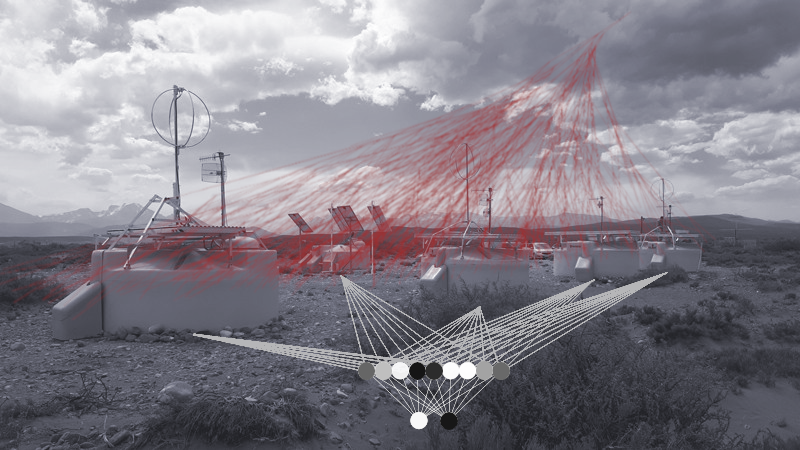
\includegraphics[height=8.53cm]{cover/cover.png}};

		\node[anchor=north] at ($(pagetopcenter) + (0mm,-\tpborder - 180mm)$)
		{
			\begin{minipage}{160mm}
				\centering
				\tpfont
				\Large Master's thesis by\\
				\vspace*{0.3cm}
				\huge\thesisauthor\\
				\vspace*{0.3cm}
				\Large at the \thesisinstitute
			\end{minipage}
		};

		\node[anchor=south] at ($(pagebotcenter) + (0mm,\tpbotborder + 20mm)$)
		{
			\begin{minipage}{160mm}
				\centering
				\tpfont
				\Large

				\begin{tabular}[ht]{l c l}
					First Reviewer: & \hfill & \thesisreviewerone\\
					Second Reviewer: & \hfill & \thesisreviewertwo\\
					% Supervisor: & \hfill & \thesisadvisorone\\
				\end{tabular}

				\vspace*{1cm}

				\large{Processing time: \thesistimestart \hspace*{0.25cm} -- \hspace*{0.25cm} \thesistimeend}
			\end{minipage}
		};

		\node [anchor=west] at ($(current page.south west) + (\tpbinding + \tpborder + \tpborderradius, \tpbotborder - 0.5 * \tpborder)$) {\tpfont\tiny{KIT – The Research University in the Helmholtz Association }};

		\node [anchor=east] at ($(current page.south east) + (-\tpborder - \tpborderradius, \tpbotborder - 0.5 * \tpborder)$) {\tpfont\large{\textbf{www.kit.edu}}};
	\end{tikzpicture}
\end{titlepage}

	% % !TEX root = ../thesis.tex

\chapter*{Review and Declaration}
\thispagestyle{empty}
\vspace*{\fill}
\noindent
This thesis has been accepted by the first reviewer of the master thesis.

\vspace{2cm}\noindent
\textit{Karlsruhe, \thesistimehandin}
\begin{flushright}
    \begin{tabular}{m{5cm}}
        \\ \toprule
        \centering\thesisreviewerone \\
    \end{tabular}
\end{flushright}
\vspace*{\fill}
\noindent
I declare that the work in this thesis was carried out in accordance with
the requirements of the university's regulations and that it has not been
submitted for any other academic award. Except where indicated by specific
reference in the text, the work is the candidate's own work. Work done in
collaboration with, or with the assistance of, others is indicated as such.

\vspace{2cm}\noindent
\textit{Karlsruhe, \thesistimehandin}
\begin{flushright}
    \begin{tabular}{m{5cm}}
        \\ \toprule
        \centering\thesisauthor \\
    \end{tabular}
\end{flushright}

	\todo{Abstract}

	\TableOfContents

	% \MainMatter

	% %! TEX root = ../thesis.tex

\chapter{Introduction}
\label{chap:introduction}


From bit flips in computer hardware giving one candidate an impossible number of votes in a federal election \cite{cosmicraybitshift}, to full-scale extinction 
events considerably reducing the biodiversity on earth  during prehistoric times \cite{melott2004did, fields2020supernova}, the influence that cosmic rays have on
our day-to-day life ranges from the smallest to biggest imaginable scales.

These incredibly energetic particles are of singular interest to physicists. Not only is this because of to the information they carry about the environment near 
distant stars and galaxies, but also due to their unmatched energy distribution, which is unachievable with earth-based particle accelerators. The relativistic 
messengers from outer space help us test interaction models, push the frontier of ultra-high-energy physics and teach us of our galactic and extragalactic 
neighbourhood.

The Pierre Auger Observatory is a world-leading experiment designed to detect cosmic rays of the highest energies. It achieves this by observing extensive air 
showers in the atmosphere and drawing conclusions based on measured data. A hybrid detection approach refines the accuracy with which arrival direction, energy, 
and the type of a primary particle are reconstructed. The larger of the two available detectors is the surface detector, which is sensitive to the shower footprint
on earth. It consists of 1600 individually operating stations in an isometric triangular grid with unit spacing \SI{1.5}{\kilo\meter}.

With this compartmentalized structure, each station determines autonomously which information to forward to a central data acquisition system. This is realised via
a hierarchy of trigger algorithms that scan the measured data locally for each detector. While these triggers are fully efficient at the tail end of the energy 
spectrum, shower cascades of lower energies $E \lesssim 10^{18}$ are seldomly detected. 

In an attempt to extend the sensitivity of the surface detector to lower energies, the following thesis revisits the current trigger algorithms. Possible 
designs of new triggers based on deep neural networks are discussed, and the overall detection sensitivity is examined with a focus on implementability in the 
local station software.

With more sensitive triggers, more candidate shower events will be recorded. This paves the way for newfound analysis of the cosmic ray energy spectrum, and might
enable detection of exotic primaries like photon- or neutrino cosmic rays. Such discoveries will be certain to send waves through the community of astroparticle 
physics.

The structure of this thesis offers a summary of cosmic ray physics and atmospheric particle cascades in \autoref{chap:physical-background} and 
\autoref{chap:extensive-air-showers}. The Pierre Auger Observatory is introduced in \autoref{chap:auger-observatory}. Supplementary information regarding the 
implementation of neural networks and discussion of training data can be found in  \autoref{chap:neural-networks} and \autoref{chap:neural-network-data}. 
\autoref{chap:classical-triggers} and \autoref{chap:neural-network-triggers} are dedicated to an in-depth description of the current trigger implementations and 
newly developed triggers based on machine learning. The results of the analysis are summarized in \autoref{chap:summary-and-conclusions}



	% %! TEX root = ../thesis.tex

\chapter{Physics of cosmic rays}
\label{chap:physical-background}

The term cosmic ray is used in the context of particles that travel through space close to the speed of light. Their kinetic energy far exceeds their rest mass, 
and ranges from $\mathcal{O}(\SI{}{\giga\electronvolt})$ for solar particles to energies exceeding $10^{20}$\SI{}{\electronvolt} for atoms of extragalactic origin. 
The latter are typically referred to as \textbf{U}ltra \textbf{H}igh \textbf{E}nergy CRs (UHECRs) in literature.

This chapter aims to introduce the general physical principles needed to describe cosmic rays. For this purpose, an overview of the origin of CRs is presented in
\autoref{sec:cr-acceleration}, discussions regarding their propagation in space, the resulting primary and energy composition are given in 
\autoref{sec:cr-propagation}, \autoref{sec:cr-composition} and \autoref{sec:cr-energy-spectrum} respectively. Immediately following is a summary of the discovery of cosmic rays in \autoref{sec:cr-history}.

\section{History}
\label{sec:cr-history}

A first hint at the existance of high-energy particles in the upper atmosphere was given by Hess in 1912, who found that the discharge rate of an electroscope is 
altitude-dependant. Millikan coined the term cosmic "rays" for these particles, as he argued the ionizing radiation must be part of the electromagnetic spectrum 
\cite{millikan1928origin}. This was later, at least partially, falsified with the discovery of the east-west effect \cite{johnson1938note}. Hess' observation 
however withstood the tests of time and was ultimately recognized with the Nobel prize in physics in 1936 \cite{nobelprize1936}. Two years later, in 1938, Pierre 
Auger showed via coincidence measurements that cosmic rays in fact originate from outer space, and gave a first description of extensive air showers 
\cite{auger1939extensive}. Another 60 years later, the Pierre Auger collaboration would adopt his experimental setup and name in their search for cosmic rays of 
the highest energies.

In the meantime, numerous results from different cosmic ray detectors all over the globe have helped propel the related fields of particle physics, astro physics 
and cosmology to new insights. Observations from cosmic ray physics serve as a valuable cross-check to the hadronic interaction models developed e.g. at CERN 
\cite{ostapchenko2007status}. New theories modeling the final moments in the life of stars have arisen thanks to results from e.g. Kamiokande 
\cite{goldman1988implications}. Last but not least, publications by the Pierre Auger collaboration regarding the CR energy spectrum and flux help refine knowledge of 
our cosmic neighbourhood \cite{abraham2010measurement, aab2015searches}.

\section{Acceleration}
\label{sec:cr-acceleration}

Following the detection of a cosmic ray on earth, the logically following questions are "where did it originate from?", and "how was it accelerated?". It is clear 
that particles with extreme energies must be created under extreme conditions. In particular regions with large \textbf{e}lectro\textbf{m}agnetic (EM) fields, either 
in field strength or spatial extent, play a big role in the acceleration of CRs for reasons listed in the following pages. Several acceleration mechanisms have been identified.

\subsection{Diffusive shock acceleration (Fermi I)}
\label{ssec:cr-fermi-i}

\textbf{S}uper \textbf{N}ova \textbf{R}emnants (SNR) typically feature a plasma sphere propagating outwards from the former stars core into the 
\textbf{I}nter \textbf{S}tellar \textbf{M}edium (ISM), in this region of plasma any magnetic field lines will be comoving, according to Alfvén's theorem 
\cite{alfven1942existence}. First realised by Fermi, such SNR shock fronts serve as source of high-energy CRs \cite{fermi1949origin}.

If a low-energy particle is injected into the SNR shock front, it will eventually be reflected by the local $\vec{B}$-field. If the diffusion length within the
plasma is much smaller than the spatial extent of the SNR, the shock front can be modelled as a plane, and the process is analogous to an elastic reflection 
against a wall. Consequently, if $\frac{\text{d}\vec{B}}{\text{d}t} = 0$, this does not cause the particle to gain any energy, espically because 
$W = \vec{F}_\text{L} \cdot \vec{r} \propto (\vec{v}\times\vec{B})\,\cdot\,\vec{r} = 0$. However, because the $\vec{B}$-field is moving radially outward alongside 
the plasma, a net energy gain of 

\begin{equation}
\label{eq:fermi-energy-gain}
\Delta E = +\beta_\text{SNR} \cdot E_0
\end{equation}

arises, where $\beta_\text{SNR} = |\vec{v}_\text{SNR}|\,/\,c$ and $E_0$ are the velocity of the shock-front and the initial energy of the particle. From chapter 7 
in \cite{fermi1949origin} it follows that ionization losses within the shock front are not completely negligible. Hence a particle must have a sufficient energy 
such that $\Delta E$ in \autoref{eq:fermi-energy-gain} exceeds possible ionization losses. The corresponding threshold for the primary energy above which 
acceleration occurs is dubbed the injection energy, and is of the order of \SI{200}{\mega\electronvolt} for protons. 

Furthermore, because typically $\beta_\text{SNR} \leq 0.10$ a single acceleration cycle is not enough to explain the CR energies observed on earth. Instead, 
multiple cycles are needed. This requires additional, focusing $\vec{B}$-fields, provided for example by the ISM, which alter the trajectory of injected particles 
such that they can be reflected off the shock-front again.

With each cycle, the particles rigidity $R = |\vec{p}|c\,/\,q$ increases, until its gyroradius $\rho = R / |\vec{B}|$ exceeds the spatial extent of the focusing 
$\vec{B}$-field and the particle escapes into space. With an effective ejection probability $p$ per cycle, the energy after $n$ cycles and the expected flux w.r.t
energy, $\Upphi(E)$, becomes roughly

\begin{equation}
\label{eq:fermi-energy}
E(n) = E_0\;\left( 1 + \beta_\text{SNR} \right)^n.
\end{equation}

\begin{align*}
                                                        N(n) &= N_0 \;\left( 1 - p \right)^n \\
\Leftrightarrow\;\;\;\;\,\log\left( \frac{N(n)}{N_0} \right) &= n\cdot\log\left( 1-p \right) \\ 
\Leftrightarrow\qquad\qquad\qquad\;\;&\stackrel{\mathmakebox[\widthof{=}]{\eqref{eq:fermi-energy}}}{=}\;\log\left( \frac{E(n)}{E_0} \right) 
\frac{\log(1-p)}{\log(1+\beta_\text{SNR})} \\
\Leftrightarrow\qquad\qquad                             N(E) &= N_0\cdot\left( \frac{E(n)}{E_0} \right)^{\log(1 - p)\;/\;\log(1 + \beta_\text{SNR})} \\
\Rightarrow \qquad\qquad                           \Upphi(E) &= \frac{ \text{d}N }{ \text{d}E } \propto E(n)^{\alpha - 1}, \numberthis\label{eq:fermi-spectrum}
\end{align*}

where $\alpha = \frac{\log(1 - p)}{\log(1 + \beta_\text{SNR})}$ in \autoref{eq:fermi-spectrum} is a spectral coefficient whose exact value will depend on the age 
of the SNR ($\beta_\text{SNR}$ decreases with age), the injected particle (different primaries have different injection energies and ejection probabilities), as 
well as many other factors that are often not known a priori. It can however be observed that the expected spectrum is a power law in the ranges from injection energy 
to a cutoff at the highest energies, which arises due to the finite lifetime of SNRs.

Results from several studies (e.g. \cite{aab2015searches, hillas2005can, blasi2013origin}) hint that the presented first order Fermi acceleration mechanism is the 
main source of galactic CRs, extrasolar particles that originate from within the milky way, with energies ranging up to orders 
$\mathcal{O}(\SI{}{\tera\electronvolt})$.

\subsection{Stochastic scattering acceleration (Fermi II)}
\label{ssec:cr-fermi-ii}

Second order (or stochastic) Fermi acceleration is the more general case of \autoref{ssec:cr-fermi-i} and represents the original idea developed by Fermi in 
\cite{fermi1949origin}. The underlaying principle of scattering particles off plasma clouds remains unchanged. However, if the diffusion length within the cloud 
exceeds its radius of curvature, the energy gain per collision instead becomes

\begin{equation}
\Delta E \propto + \left( \beta_\text{SNR}\right)^2 \cdot E_0.
\end{equation}

Logically, this represents a much more inefficient acceleration mechanism, but is nevertheless observed in nature under certain circumstances (c.f. 
\cite{asano2015most}).

\subsection{Centrifugal acceleration in rotating $\vec{B}$-fields}
\label{ssec:cr-centrifugal-acceleration}

Some astrophysical objects such as pulsars or \textbf{A}ctive \textbf{G}alactic \textbf{N}uclei (AGNs) possess strong magnetic fields ranging from \SI{1}{\tesla}
for some AGNs \cite{daly2019black} to $\approx\SI{10}{\giga\tesla}$ for magnetars, a subset of pulsars with extremely high magnetic flux densities 
\cite{flowers1977evolution}.

If such objects rotate at an angular velocity $\Omega$, which is in general nonzero, charged particles at a radial distance $r$ from the rotation axis will undergo
centrifugal acceleration. In particular, their Lorentz factor $\gamma$ behaves like \autoref{eq:lorentz-factor-acceleration} \cite{rieger1999particle}.

\begin{equation}
\label{eq:lorentz-factor-acceleration}
\gamma := \frac{E}{m_0 c^2} = \frac{\gamma_0}{1 - \left(\frac{\Omega r}{c}\right)^2},
\end{equation}

where $m_0$ is the rest mass of the particle and $\gamma_0$ the prior Lorentz factor before acceleration. It follows that a test particle can in theory gain an
arbitrarily high energy from this process by outspiraling towards the light cylinder surface, where $\Omega\cdot r = c$. In reality however, these processes are
stopped by e.g. inverse Compton scattering at some point \cite{osmanov2007efficiency}. In any case, \cite{rieger1999particle} and \cite{osmanov2007efficiency}
conclude that values of $\gamma \approx 10^7-10^8$ are possible, corresponding to protons at $\approx\SI{10}{\peta\electronvolt}-\SI{10}{\peta\electronvolt}$ or 
iron nuclei at $\approx\SI{500}{\peta\electronvolt}-\SI{5}{\exa\electronvolt}$ energy.

\subsection{Direct electrostatic acceleration}
\label{ssec:cr-electrostatic-acceleration}

The presence of non-static $\vec{B}$-fields implies the existance of (in vacuum) comparably strong $\vec{E}$-fields and a corresponding electrical potential 
difference $\Upphi$ across different regions within the magnetosphere. A back-of-the-envelope calculation reveals that they are (neglecting constant factors) 
proportional to

\begin{align}
|\vec{E}| &\propto \frac{\Omega\;r_0}{c} \cdot |\vec{B}|, \\
\Upphi &\propto r_0 \cdot |\vec{E}|,
\end{align}

where $r_0$ is the radius of the central object rotating at an angular frequency $\Omega$. Consequently, an ion with atomic number $Z$ can be accelerated to 
energies $E = Z \cdot e \cdot \Upphi$, which can in some cases easily exceed $10^{20}\SI{}{\electronvolt}$ \cite{rieger2009cosmic}. 

Some caveats to this consideration need to be mentioned. Screening effects from plasma clouds surrounding the central body are expected to limit the electrical 
field strength, and maximum acceleration energy by extension. Additionally, losses via e.g. Bremsstrahlung have been neglected in the above calculation, limiting
the maximum attainable energy in theory even further. 

\subsection{Other types \& general classification}
\label{ssec:cr-hillas-plot}

Several acceleration mechanisms have been discussed. A plethora of other interactions that are able to accelerate elementary particles to fantastic energies remain
unmentioned, or even undiscovered, as CR physics is an active area of research. In general though the driving force behind all considered (and non-considered)
acceleration mechanisms are thought to be (electro-) magnetic fields, given their infinite range and large coupling strengths compared to other fundamental 
forces. Consequently, the maximum energy a specific CR accelerator with magnetic field $\vec{B}$ and size $L$ moving at velocity $\beta c$ can in theory provide 
for a particle with charge $Ze$ is given by the Hillas formula \cite{hillas1984origin}:

\begin{equation}
\label{eq:hillas-formula}
E_\text{max}\;[\SI{}{\peta\electronvolt}] = |\vec{B}|\;[\SI{}{\micro\gauss}] \cdot L\;[\SI{}{\parsec}] \cdot Z \cdot \beta
\end{equation}

This allows for an elegant classification of different cosmic ray sources, in part discussed on the previous pages, according to the Hillas plot shown in 
\autoref{fig:hillas-plot}.

\begin{figure}
	\centering
	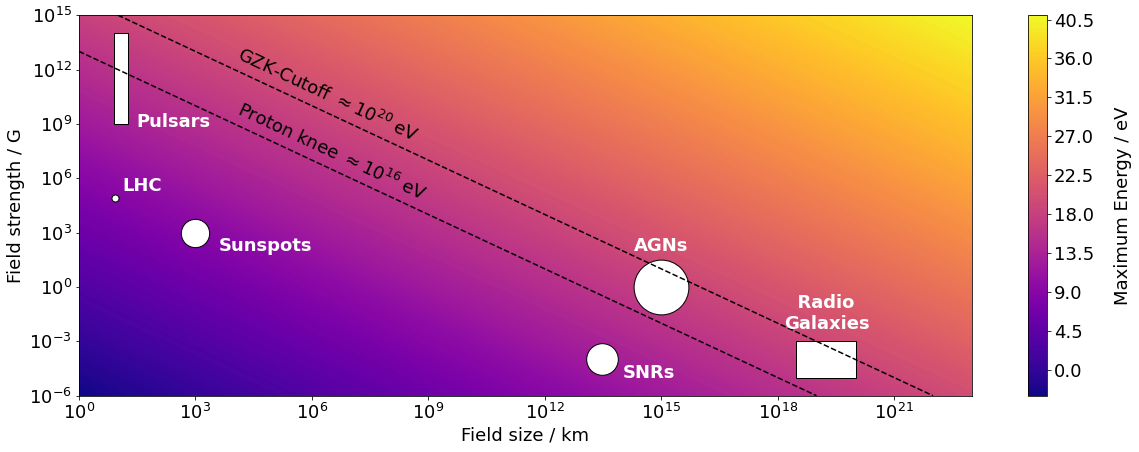
\includegraphics[width=1\textwidth]{./plots/hillas_plot.png}
	\caption{Rough estimate of field strength and size of different CR sources as well as the corresponding maximum energy estimated with 
    \autoref{eq:hillas-formula} ($\beta = Z = 1$). Isoenergetic lines mark notable points in the energy spectrum discussed in 
    \autoref{sec:cr-energy-spectrum}.}
	\label{fig:hillas-plot}
\end{figure}

\subsection{Acceleration of uncharged particles}
\label{ssec:cr-uncharged-acceleration}

Particles like neutrons, neutrinos or photons possess no electromagnetic charge $q = 0$. Assuming \autoref{eq:hillas-formula} holds in these cases, they 
should thus not appear in the CR spectrum. This is in disagreement with reality, where energies from \SI{100}{\giga\electronvolt} up to 
$\approx\SI{100}{\exa\electronvolt}$ have been observed \cite{abeysekara2018very, ishihara2016extremely}. Consequently, additional interaction channels are 
required to explain the existance of such uncharged CRs.

High energy $\gamma$-rays in particular can be created by accelerated, charged particles via Bremsstrahlung. This occurs for example during centrifugal 
acceleration near pulsars or AGNs (compare \autoref{ssec:cr-centrifugal-acceleration}). Furthermore, inverse Compton scattering with a high-energy cosmic ray can 
imply a significant energy gain for a photon \cite{jones1965inverse}.

Uncharged CRs are also frequently produced in nuclear interactions, such as e.g. deeply inelastic scattering of charged CRs with the ISM. This espically 
contributes to the CR photon spectrum, as high energy $\pi^0$ are often byproducts of such scattering processes. The uncharged pions then decay into two photons. 
Furthermore, neutrons or neutrinos can originate from interactions involving the weak force. When a proton converts to $p\rightarrow n+e^++\bar{\nu_e}$ during the 
dacy of a UHECR ion, the resulting decay products, positron, neutron and electron-antineutrino inherit the parents' energy, and are thus high energy cosmic rays as 
well.

\section{Propagation}
\label{sec:cr-propagation}

Once a cosmic ray has been observed coming from some arrival direction $(\phi, \theta)$, backtracking its' trajectory to an eventual origin is, ignoring external 
factors, in the literal sense, straight forward. It has been shown however that several effects need to be considered for an accurate treatment of CR propagation. 

For uncharged CRs ($\gamma$, $n$), this task is simple. Such particles are not deflected by cosmic $\vec{E}$ and $\vec{B}$-fields. Possible interactions either 
demand the destruction of the particle (pair production, weak decay), or occur close to the source (e.g. Compton scattering), in which case the observed arrival 
direction will still be coincident with the actual source \cite{fermi201398}. Gravitational lensing effects in some cases alter the trajectory of extragalactic 
photons. Such phenomena (if present in the first place) are however well understood in the scope of general relativity, and can be corrected for 
\cite{bartelmann2010gravitational, bartelmann2001weak}.

\subsection{Intergalactic propagation \& transport equation}
\label{ssec:transport-equation}

Contrary, charged particles ($e^\pm$, $p$, ions) propagate along non-trivial paths within galaxies due to deflections from solar- and galactic EM-fields. While the 
galactic field is coherent over large scales, numerous irregular magnetic domains, seeded in part by individual stars complicate CR propagation to essentially a 
three-dimensional random walk \cite{haverkorn2015magnetic}. It is thus challenging to pinpoint the origin of a charged cosmic ray. 

Nevertheless, related queries, such as for example the question whether or not a particle of given energy is likely to be of extragalactic origin can be answered by
examining the distribution of cosmic rays within a region of spacetime. The behaviour of a population of $n_i$ particles of type $i$ can be approximately recreated 
via the below transport equation:

\begin{equation*}
\label{eq:leaky-box-model}
\frac{\partial n_i}{\partial t} =   \underbrace{Q_i \vphantom{\left(\sum\limits_{j>i}\frac{p_{ij}}{\tau_{\text{spal.},\,j}} n_j\right)}}_\text{Source} 
 								  + \underbrace{\nabla D_i \left( \nabla n_i \right) \vphantom{\left(\sum\limits_{j>i}\frac{p_{ij}}{\tau_{\text{spal.},\,j}} n_j\right)}}_\text{Diffusion} 
								  - \underbrace{\frac{\partial k_i(E)}{\partial E} \vphantom{\left(\sum\limits_{j>i}\frac{p_{ij}}{\tau_{\text{spal.},\,j}} n_j\right)}}_\text{Energy} 
								  - \underbrace{\left( \frac{n_i}{\tau_{\text{spal.},\,i}} - \sum\limits_{j>i} \frac{n_j\,p_{ij}}{\tau_{\text{spal.},\,j}} \right)}_\text{Spallation}
								  - \underbrace{\left( \frac{n_i}{\tau_{\text{rad.},\,i}} - \sum\limits_{j>i} \frac{ n_j\,d_{ij}}{\tau_{\text{rad.},\,j}} \right)}_\text{Weak decay}
\end{equation*}

\begin{itemize}
	\item \textbf{Source} $Q_i$ :

	The source term is responsible for the creation of CR particles (of type $i$). The exact form of $Q_i$ will depend on the considered creation process. For 
	example, the near instantaneous creation of $n_\gamma$ photons in a \textbf{G}amma-\textbf{R}ay \textbf{B}urst (GRB) at time $t_0$ and location $\vec{r_0}$ can 
	be modelled like $Q_\gamma = n_\gamma \; \delta(\vec{r} - \vec{r_0}) \, \delta(t - t_0)$.

	\item \textbf{Diffusion} $\nabla D_i \left( \nabla n_i \right)$ :

	The random walk mentioned above is accounted for in the diffusion term, which takes a similar form to the Stokes-Einstein equation. The diffusion 
	coefficient(s) $D_i$ in the most general case take a tensor form due to anisotropic diffusion in different directions. Furthermore, $D_i$ is 
	different for each particle type, as the deflecting EM-fields couple to the respective charges $q_i$, which need not be equal in principle.

	\item \textbf{Energy loss} $\partial k_i(E)\,/\,\partial E$ :

	During propagation, a cosmic ray can interact with the ISM, and lose energy in the process. If this happens often enough, the CR is eventually thermalized and 
	does not contribute to the population $i$ any longer. Different interaction channels for different CR types $i$ require different loss models $k_i(E)$ for each 
	type. 

	\item \textbf{Spallation} $\left( n_i\,/\,\tau_{\text{spal.},\,i} - \sum n_j\,p_{ij}\,/\,\tau_{\text{spal.},\,j} \right)$ :

	Nuclear spallation describes the process of violent disintegration of a target nucleus upon being struck by an energetic projectile. The resulting fragments
	can retain energies up to the projectiles energy. The spallation term in the transport equation considers both the destruction (first term), as well as 
	creation (second term) of CRs $i$ from heavier types $j$. It is assumed that spallation from type $j \rightarrow i$ occurs at a constant probability of 
	$p_{ij}$ in a characteristic time frame $\tau_{\text{spal.},\,j}$.

	\item \textbf{Weak decay} $\left( n_i\,/\,\tau_{\text{rad.},\,i} - \sum n_j\,d_{ij}\,/\,\tau_{\text{rad.},\,j} \right)$ :

	If a particle $j$ is weakly unstable ($\tau_{\text{rad.},\,i} < \infty$) there is a nonzero chance $d_{ij}$ it decays into a daughter nuclei of some type $i$ 
	during propagation. The decay term reflects this and describes both decay from heavier and decay into lighter nuclei.
\end{itemize}

Insights to the physical implications of this parametrization can be gathered from a simplified example. Consider the case of a galaxy with height $2H$ and width 
$W$. It is $H \ll W$, and thus only diffusion along the $\pm z$-direction will be examined. Considering $n_0$ protons located at $z=0$ initially, and ignoring 
interactions with the ISM, the transport equation reduces to the first two terms, with $D = \left( 0, 0, D_z \right)^\text{T}$ and 
$Q = n_0\,\delta(z)\,\delta(t_0)$.

\begin{figure}
	\begin{subfigure}[b]{0.32\textwidth}
		\centering
		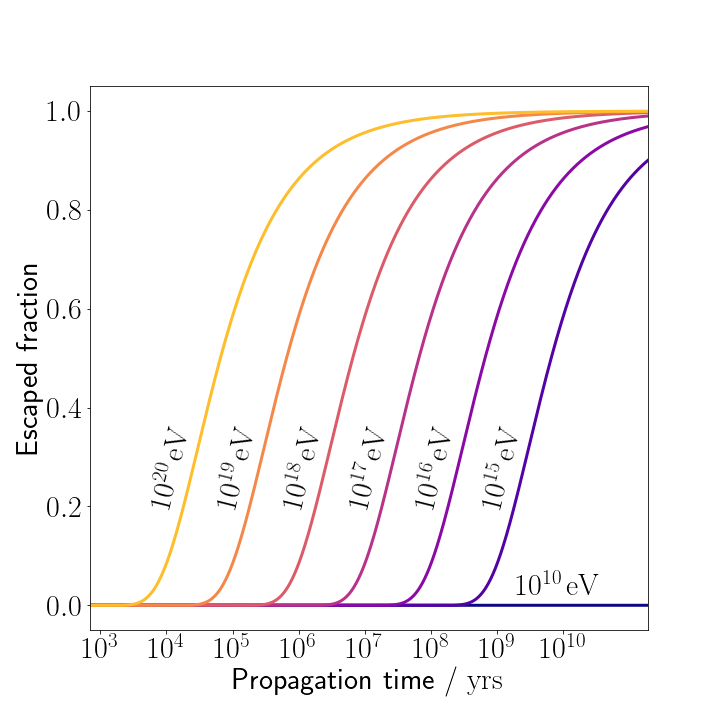
\includegraphics[width=\textwidth]{./plots/galactic_diffusion.png}
		\caption{\textbf{Escape fraction}}
		\label{fig:escape-fraction}
	\end{subfigure}
	\hfill
	\begin{subfigure}[b]{0.68\textwidth}
		\centering
		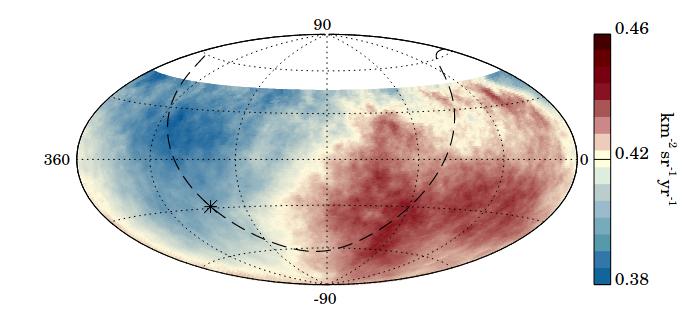
\includegraphics[width=\textwidth]{./plots/auger_dipole.png}
		\caption{\textbf{AD anisotropy}}
		\label{fig:ad-anisotropy}
	\end{subfigure}
	\caption{\textbf{(a)} $r_\text{esc.}(t)$ according to \autoref{eq:escape-fraction} for protons of different energies.\\ \textbf{(b)} Dipole in the arrival
	direction of CRs with $E>\SI{8}{\exa\electronvolt}$. Image copied from \cite{pierre2017observation}.}
\end{figure}

It can quickly be verified that a solution to the transport equation in this case is given by a normal distribution with mean $\upmu = 0$ and standard deviation 
$\sigma = \sqrt{2D_zt}$. The diffusion coefficient $D_z$ is a measure of how quickly the population spreads out (along the $\pm z$-direction). According to 
\cite{skilling1970diffusion}, $D_z$ can be parametrized via the particles energy $E_p$, and characteristics of the present $\vec{B}$-fields.

\begin{equation}
	\label{eq:diffusion-coefficient}
	D_z =\frac{1}{3}\,\frac{E_p}{m_p\,c^2}\cdot\frac{|\vec{B}|\cdot\langle L_{\vec{B}}\rangle}{\sqrt{\upmu_0\,\rho_\text{ISM}}},
\end{equation}

where $\langle L_{\vec{B}} \rangle$ is the characteristic length scale of deflecting $\vec{B}$-fields, $\upmu_0$ and $\rho_\text{ISM}$ are the magnetic vacuum 
permeability and density of the interstellar medium respectively. After some time $t$, a fraction $r_\text{esc.}(t)$ of particles will have a $z$-coordinate 
$|z| > H$, and exit the disc consequently. In reality, this is not equivalent to the particle leaving the galaxy, as large-scale halo structures extend above and 
below the visible disc \cite{searle1978compositions}. These halos are ignored here. $r_\text{esc.}(t)$ can thus be calculated according to 
\autoref{eq:escape-fraction}. For some selected energies, a plot of the escaping ratio over time is offered in \autoref{fig:escape-fraction}.

\begin{equation}
\label{eq:escape-fraction}
r_\text{esc.}(t) := 1 - \int\limits_{-H}^{H} \frac{n(z,t)}{n_0}\,\text{d}z
\end{equation}


It can be concluded that low energy CRs do not travel outside their host galaxy within reasonable timeframes. Meanwhile UHECRs with energies exceeding 
$E>10^{18}\,\text{eV}$ escape swiftly on ballistic trajectories and are thus likely have an extragalactic origin, not last also due to the limited energies that CR
sources in the milky way can provide.

This observation is consistent with a dipole in the \textbf{A}rrival \textbf{D}irection (AD) of UHECRs observed by the Pierre Auger observatory. The dipole points
roughly in the opposite direction of the galactic core, marked with an asterisk in \autoref{fig:ad-anisotropy}.

\subsection{Extragalactic propagation \& GZK-Cutoff}
\label{ssec:gzk-cutoff}

In the last paragraph the (likely) extragalactic origin of UHECRs was discussed. Such particles must traverse millions of lightyears of extragalactic space before
inducing a large air shower on earth. As the energy of these primaries increases above the \textbf{G}reisen-\textbf{Z}atsepin-\textbf{K}usmin threshold (GZK),
their propagation through space is thought to be severely impeded. At energies above $\approx10^{20}\,\text{eV}$ the \textbf{C}osmic \textbf{M}icrowave
\textbf{B}ackground (CMB) consisting of photons in the microwave range are blueshifted to energies $E_\gamma > \SI{300}{\mega\electronvolt}$. A proton with the 
corresponding energy can thus absorb such CMB photons and convert to its' excited spin state, the $\Delta^+$-baryon. The $\Delta^+$-baryon decays nearly 
instantanouely to (for example) the ground state again, by radiating away a $\pi^0$ and losing energy in the process \cite{PDG}. 

The mean free path of this interaction, also labelled GZK horizon is both energy- and primary-dependant. For \SI{75}{\exa\electronvolt} protons, it is 
$\approx \SI{100}{\mega\parsec}$ \cite{greisen1966end}. Cosmic rays exceeding the GZK threshold should ergo not be observed from faraway sources, and an overall 
reduction in flux at these energies should be recorded \cite{zatsepin1966j}.

Indeed, results published by the Auger collaboration (see \autoref{sec:cr-energy-spectrum}) are consistent with this assumption. Whether or not the GZK-supression
is the main cause for this soft spectrum at the highest energies remains unclear for now, but might be answered with the ongoing 
AugerPrime upgrade of the Pierre Auger observatory. 

\section{Composition}
\label{sec:cr-composition}

The composition of CRs largely mirror the relative abundancies of elements in the universe with some noteable exceptions shown in \autoref{fig:cr-composition}.
Elements like beryllium (Be) or vanadium (V) are atypical products of supernovae and thus not as common as e.g. oxygen (O) \cite{gamezo2005three, cowan2004r} in
the solar system. This leads to a dip in the corresponding abundancy spectrum. The same dip is not observed in CR primary abundancies. While it is a priori 
existant upon creation of cosmic rays, it gradually gets "filled up" via e.g. spallation processes during their propagation until an equilibrium state is reached.

This equilibrium state depends sensitively on the characteristic age of cosmic rays, i.e. the mean travel time until a particle escapes the galaxy. Measuring CR 
composition hence enables the estimation of this parameter. Such an analysis is conducted in \cite{garcia1977age}, where it is found that the observed abundancies 
are consistent with a characteristic age of \SI{1.7e7}{\year} for such high energy particles.

Contrary, hydrogen (H) and helium (He) are underrepresented (w.r.t their natural abundancy in the solar system) in cosmic ray particles. This is likely due to the 
comparably high ionization energy of both elements, which leads to less readily available hydrogen/helium ions. Since the acceleration mechanisms discussed in 
\autoref{sec:cr-acceleration} all couple to the net charge $q$ of a particle, unionized hydrogen and helium are not accelerated \cite{wang2002measurement}.

\begin{figure}
	\centering
	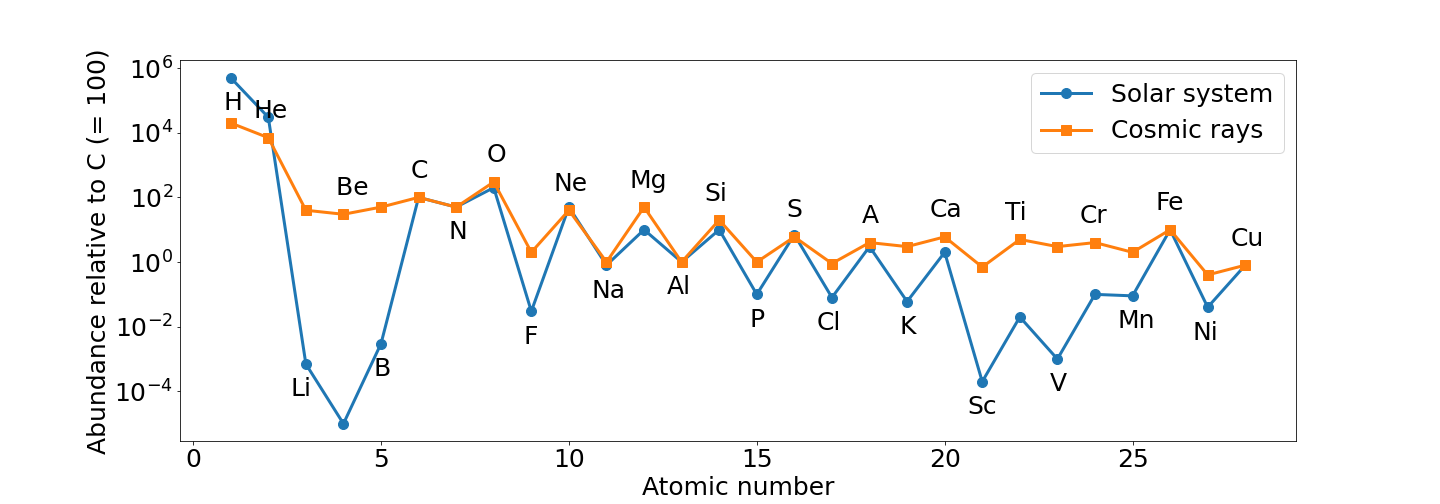
\includegraphics[width=1\textwidth]{./plots/cosmic_ray_composition.png}
	\caption{Composition expressed as abundancy relative to carbon for different sources. The ragged, alternating structure stems from an increased stability of 
	nuclei with an even amount of protons (c.f. for example \cite{kirson2008mutual}). Data from \cite{gaisser2016cosmic}}
	\label{fig:cr-composition}
\end{figure}

\section{Energy spectrum}
\label{sec:cr-energy-spectrum}

\begin{figure}
	\centering
	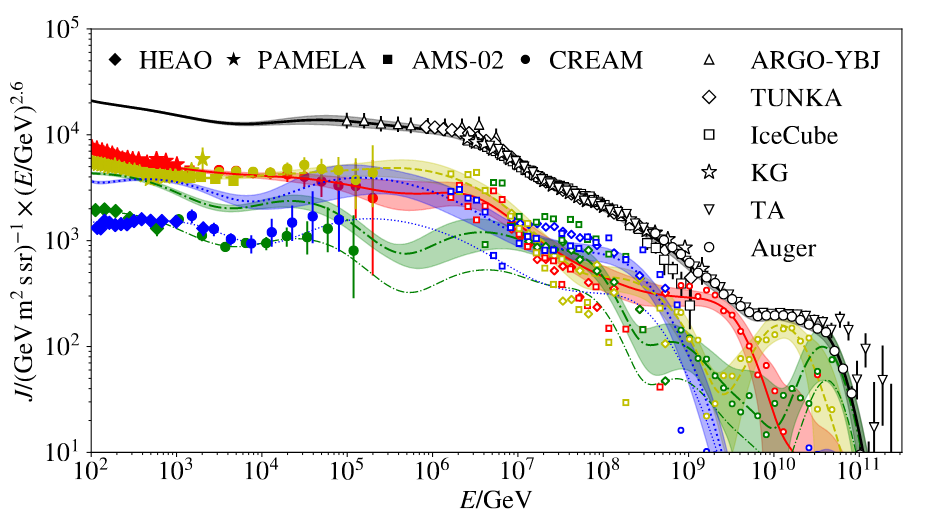
\includegraphics[width=1\textwidth]{./plots/cosmic_ray_spectrum.png}
	\caption{Measurements of the cosmic ray flux, multiplied by a factor $E^{2.6}$ for all types (black), and broken down by primary. Shown are protons (red), 
	helium (yellow), oxygen (green) and iron (blue). Plot adopted from \cite{dembinski2017data}.}
	\label{fig:cr-energy-spectrum}
\end{figure}

It has been discussed in \autoref{sec:cr-acceleration} that the expected CR flux w.r.t energy for supernova remnants is a powerlaw in the rough range of 
$\SI{200}{\mega\electronvolt} < E \lesssim \SI{100}{\tera\electronvolt}$. Observations by various experiments extend this result to even higher energies. Their 
combined results are shown in \autoref{fig:cr-energy-spectrum}. However, while the general assumption of a powerlaw $\Upphi(E)\propto E^\alpha$ holds over a large
range of energies, kinks and other feature in the spectrum indicate that the spectral index $\alpha$ is not uniform, and instead a function of energy. The 
approximate form of $\alpha(E)$ will be discussed in the following by examining several key regions of the energy spectrum. 

\TODO{reformat this in some better way}

\subsection{The proton knee; $\alpha(E < 10^{15}\,\SI{}{\electronvolt}) = 2.7 \rightarrow \alpha(E > 10^{15}\,\SI{}{\electronvolt}) = 3.0$}
\label{ssec:cr-proton-knee}

Below an energy of $\approx \SI{1}{\peta\electronvolt} = 10^6\,\SI{}{\giga\electronvolt}$, it is $\alpha(E)\approx 2.7$, while above a spectral index of 
$\alpha(E)\approx 3.0$ is found \cite{gaisser2016cosmic}. This softening of the spectrum (i.e. fewer particles of higher energy) could be attributed to several
effects.

\begin{itemize}
	\item \textbf{Dark matter channel} (partially falsified)

	\textbf{W}eakly \textbf{I}nteractive \textbf{M}assive \textbf{P}articles (WIMPs) are a popular candidate for \textbf{D}ark \textbf{M}atter (DM), as they 
	correctly estimate the cosmological evolution of the universe \cite{klypin1993structure}. A WIMP with a sufficiently high mass could explain the kink in the 
	energy spectrum. CRs with $E > m_\text{WIMP}c^2$ could in theory produce DM in deeply-inelastic scattering processes. The degree of steepening in the spectrum 
	is a measure for how readily the process $X \rightarrow \text{WIMP} + Y$ occurs. The steeper the spectrum gets, the more particles are converted to DM, and the
	higher the corresponding cross sections are. Most theories involving WIMP creation can be excluded, since detectors at earthbound particle accelerators should 
	have observed DM production at the observed steepening from $2.7$ to $3.0$ \cite{donato2009constraints}.

	\item \textbf{Escape during propagation}

	While the analysis in \autoref{ssec:transport-equation} concludes that the escape time for $\,10^{15}\,\text{eV}$ protons to leave their host 	galaxy is at 
	least of the order ${10^{8}}\,\text{yr}$ (compare \autoref{fig:escape-fraction}), the calculations leading to this result are extremely simplified. If a more 
	accurate treatment finds that particles with rigidities corresponding to the relevant energies are no longer confined by galactic magnetic fields, the kink 
	could originate from particles leaving the milky way and not contributing to the flux observed on earth any longer.

	\item \textbf{Limited source energy}

	A last possible explanation might lie in \autoref{eq:hillas-formula}. A prevalent acceleration mechanism for CRs below $10^{15}\SI{}{\electronvolt}$, such as 
	shock acceleration in SNRs for example, might not be able to provide energies exceeding this threshold due to physical constraints. The spectrum above the 
	proton knee is thus populated by CRs that originate from different acceleration mechanisms with differen relations $\alpha(E)$.
\end{itemize}

\subsection{The iron knee; $\alpha(E < 10^{17}\,\SI{}{\electronvolt}) = 3.0 \rightarrow \alpha(E > 10^{17}\,\SI{}{\electronvolt}) = 3.0$}
\label{ssec:cr-iron-knee}

The spectrum exhibits various similar kinks at slightly higher energies than the one discussed in \autoref{ssec:cr-proton-knee}, while it is assumed that they are 
ultimately caused by the same physical principles, each one corresponds to a different primary particle. Representatively, the iron knee at 
$E \approx 10^{17}\,\text{eV}$ is discussed here. 

Because iron has both a higher mass and charge ($Z = 26$, $A = 56$) compared to the proton ($Z = A = 1$), different processes couple to the different nuclei with 
disparate strength. In particular, an iron core has a higher magnetic rigidity $R \propto \frac{A}{Z}$ than a proton of equivalent energy. This is explained by the
fact that, while the iron core experiences a larger Lorentz force ($\propto Z$), the resulting acceleration ($\propto \frac{Z}{A}$) is not as strong due to a
disproportionally larger mass ($\propto A$). It is thus logical to expect differences in the creation, propagation, and shower characteristics 
(see \autoref{ssec:superposition-principle} for details) of different CR primary particles. By extension, the spectral index $\alpha(E)$ should be contrasting for 
each distinct particle type $i$, giving rise to different fluxes $\Upphi(E)_i$, which is confirmed by \autoref{fig:cr-energy-spectrum}.

The ultimate cause of the different knees remains unknown currently. In the context of the ongoing AugerPrime upgrade, the Pierre Auger observatory will scan the
energy spectrum at higher precision \cite{castellina2019augerprime}. This will allow to test whether the location of the various kinks scale with $A$ or with $Z$, 
and consequently shed light on the processes giving rise to these features.

\subsection{The Ankle $E \approx 10^{18}\,\SI{}{\electronvolt}$}
\label{ssec:cr-ankle}

At an energy of roughly $\approx\SI{1}{\exa\electronvolt} = 10^9\,\SI{}{\giga\electronvolt}$ an inflection point is found, where the spectrum hardens again from an 
index $\alpha(E) = 3.0$ to $\approx 2.7$. This might mark the final transition from predominantely galactic to intergalactic cosmic rays. If intergalactic CR 
sources such as AGNs have a harder spectrum (but lower luminosity) than galactic sources, the ankle could be well explained by a smooth transition from the latter to 
the former spectrum \cite{aloisio2007dip}. Other explanations focus on a change of the primary composition, which seems to be apparent in 
\autoref{fig:cr-energy-spectrum} at the correct energy \cite{allard2012extragalactic}. In any case, more data needs to be gathered to come to an informed 
conclusion on the ultimate cause.

\subsection{The suppression $E \approx 10^{20}\,\SI{}{\electronvolt}$}
\label{ssec:cr-cutoff}

At energies beyond $10^{20}\,\text{eV}$ a sharp drop in the flux can be noted. This represents the tail end of the spectrum, beyond which events are so rare that 
cosmic ray observatories can mostly just identify upper limits with their available statistics. The cause for the drop is actively debated, and might lie in the 
GZK cutoff discussed in \autoref{ssec:gzk-cutoff}. Another explanation might be that the tail end represents the point at which even the largest and most powerful
(in terms of energy) CR sources in the universe are not able to accelerate particles any further (c.f. \autoref{fig:hillas-plot}). 
	% %! TEX root = ../thesis.tex

\chapter{Extensive air showers}
\label{chapter:extensive-air-showers}

Consider a high energy cosmic ray impinging on earth. The questions pertaining to where it might originate from and how it has gained so much kinetic energy have 
been answered in the preceding \autoref{chap:physical-background}. In the following, the particle cascades resulting from the particle interacting in the upper
atmosphere will be examined. This is done in a two-fold way. The underlaying principles will be explained via considering a particle carrying no SU$(3)$-color 
charge in \autoref{sec:heitler-model}. The more general treatment for hadronic showers is then found in \autoref{sec:heitler-matthews-model}. As supplementary 
information, the effect of different hadronic primaries is discussed in \autoref{sec:superposition-principle}.

\section{Electromagnetic showers}
\label{sec:heitler-model}

\begin{figure}
	\begin{subfigure}[b]{0.4\textwidth}
		\centering
		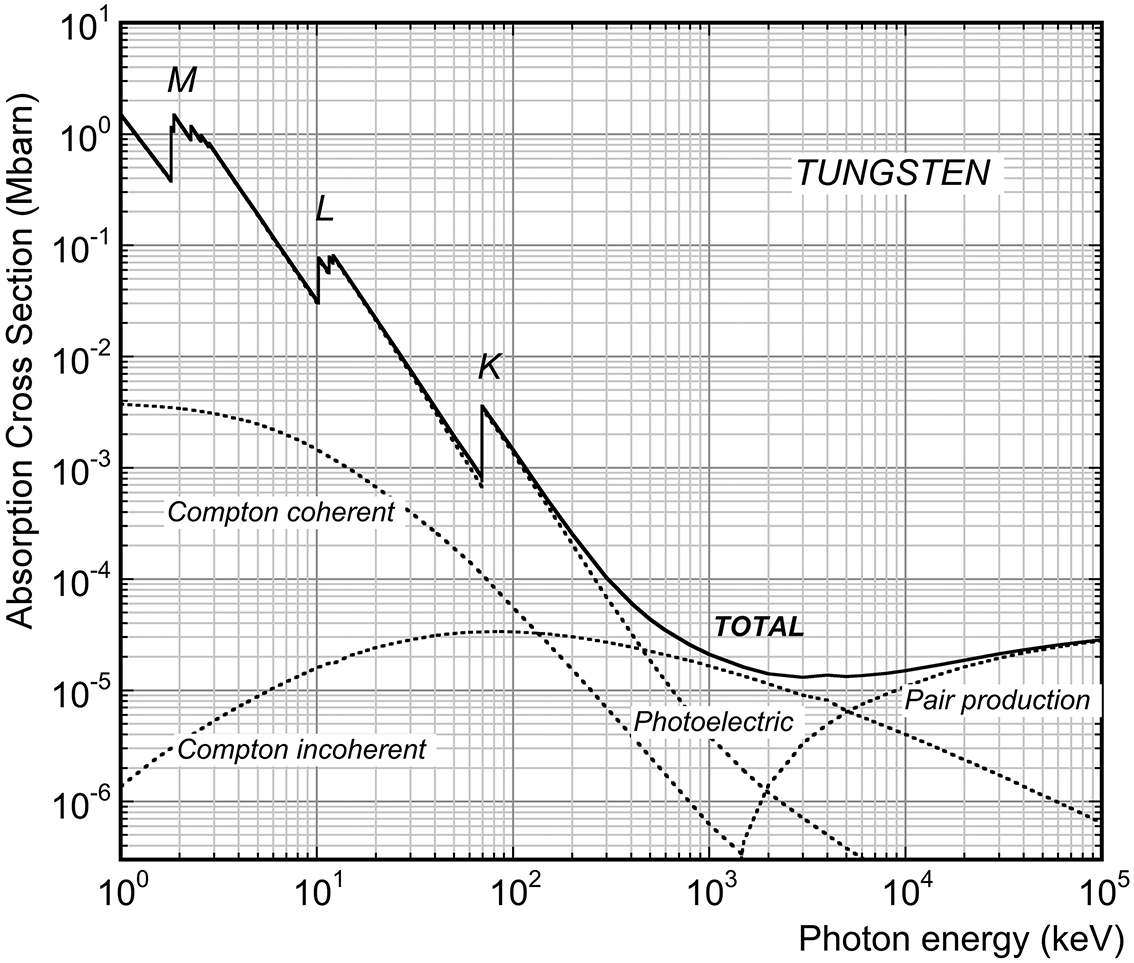
\includegraphics[width=\textwidth]{./plots/photon_cross_section.png}
		\caption{$\mathbf{\gamma}$\textbf{ interactions}}
		\label{fig:gamma-interactions}
	\end{subfigure}
	\hfill
	\begin{subfigure}[b]{0.6\textwidth}
		\centering
		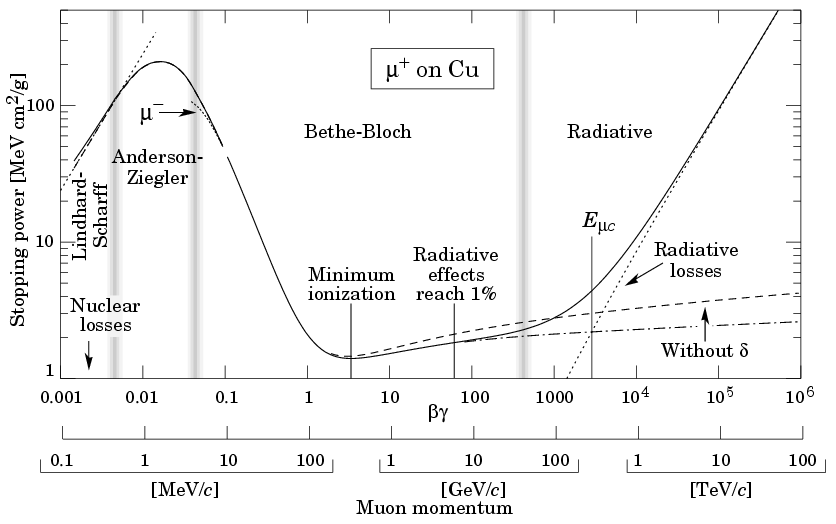
\includegraphics[width=\textwidth]{./plots/electron_ionisation_loss.png}
		\caption{$\mathbf{e^\pm}$\textbf{ interactions}}
		\label{fig:electron-interactions}
	\end{subfigure}
	\caption{\textbf{(a)} Cross section for different energy loss processes of a photon in tungsten. The sudden spikes correspond to the transition energy of 
	increasingly higher-energy electron shells. From \cite{chen2007interactions}. \textbf{(b)} Stopping power of copper, representatively on an antimuon $\upmu^+$, 
	with respect to its' momentum. Plot adopted with changes from \cite{meroli2017straggling}.}
	\label{fig:ionization-losses}
\end{figure}

The dominating interaction of $E > \SI{10}{\mega\electronvolt}$ photons in matter is $e^+e^-$ pair production, whereas for electrons/positrons the creation of a
$\gamma$ via bremsstrahlung prevails at high energies. This is shown in \autoref{fig:ionization-losses}. Consequently, an entire cascade of electrons, positrons 
and photons can emerge from a single primary particle, as realised by Heitler in \cite{heitler1984quantum}. 

Of particular interest in these showers are, apart from the primary particles energy $E_0$ and arrival direction $(\Upphi, \theta)$, the atmospheric depth 
$X_\text{max}$ at which it reaches its' maximum multiplicity, as well as the \textbf{L}ateral \textbf{D}istribution \textbf{F}unction (LDF), that parametrizes the 
distribution of particles along the shower axis. An important variable that influences both values is the radiation length $X_0$. It represents the characteristic
length at which an $e^\pm$ loses $1-\frac{1}{e}\approx63\%$ of its energy. It also corresponds to the mean free path of a photon in matter up to a factor $7 / 9$ 
\cite{gupta2010calculation}. Neglecting said factor and assuming that new particles on average inherit half of the original energy, describing the multitude of 
particles contained in an electromagnetic shower becomes a counting exercise in the context of the Heitler-model.

With each radiation length, the number of particles $N$ in the shower double, while the energy per particle $E_\text{pp}$ halves. After traversing an atmospheric 
depth of $n\cdot X_\text{max}$, typically measured in \SI{}{\gram\per\centi\meter\squared}, they consequently read

\begin{equation}
\label{eq:heitler-parameters}
N(n) = 2^n, \qquad E(n) = \frac{E_0}{2^n}.
\end{equation}

After some time, the energy of each individual particle $E_\text{PP}$ will have diminished by so much that other processes will dominate over bremsstrahlung and 
pair production. This occurs at the critical energy $E_c$ below which the shower rapidly stops creating new particles and dies out as a result. It follows via 
\autoref{eq:x-max} and \ref{eq:n-max} that both $X_\text{max}$ as well as $N_\text{max}$ increase with $E_0$. The multiplicity arising from 
these assumptions alongside a stylized propagation of the thus created shower is represented in \autoref{fig:heitler-model}. 

\begin{align*}
E_\text{PP}\,(n_\text{max}) &\stackrel{!}{=} E_c \stackrel{\eqref{eq:heitler-parameters}}{=} \frac{E_0}{2^{n_\text{max}}}\\
\Leftrightarrow \qquad \qquad n_\text{max} &= \left\lfloor \log_2 \left( \frac{E_0}{E_c} \right) \right\rfloor \\[7pt]
\Rightarrow \qquad \qquad\!\! X_\text{max} &= n_\text{max}\cdot X_0 = \left\lfloor \log_2 \left( \frac{E_0}{E_c} \right) \right\rfloor. \numberthis\label{eq:x-max} \\
\Rightarrow \qquad \qquad\!\! N_\text{max} &= 2^{n_\text{max}} = \left\lfloor \frac{E_0}{E_c} \right\rfloor. \numberthis\label{eq:n-max}
\end{align*}

\begin{figure}
	\centering
	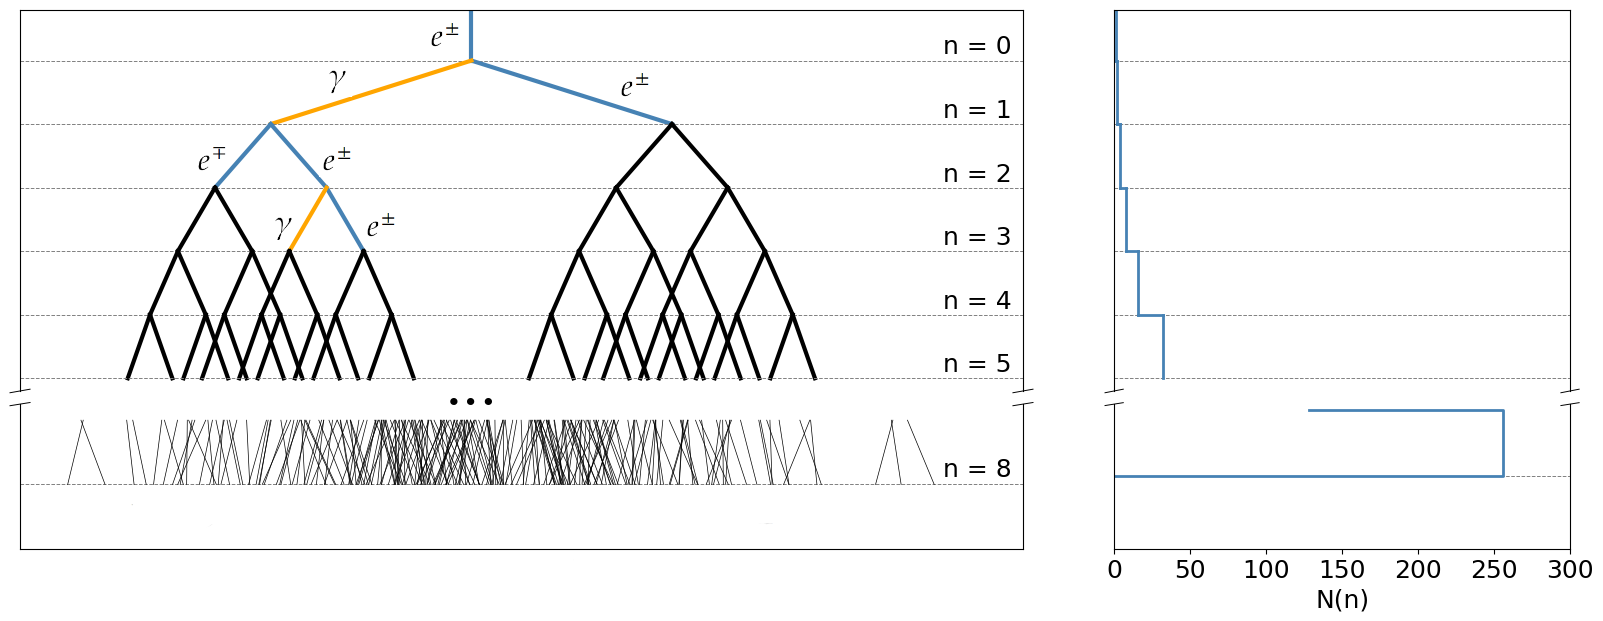
\includegraphics[width=\textwidth]{./imgs/heitler_shower.png}
	\caption{Shown on the left is the stylized propagation of an extensive air shower through the atmosphere according to the Heitler-model, quantized in units
	of $X_0$. The energy of the primary particle is of order $2^8\cdot E_c$, which allows for 8 bifurcation steps, and $N_\text{max}=256$ shower particles. The
	multiplicity of the shower after each step is shown in the right subplot.}
	\label{fig:heitler-model}
\end{figure}

The number of particles at a given distance from the shower axis (y-axis in \autoref{fig:heitler-model}) is essentially random, but follows a statistical basis,
the lateral distribution function. The LDF can either be derived approximately from first principles \cite{kamata1958lateral} or empirically, as is done in 
\cite{greisen1960cosmic}. The latter arrives at a closed form approximation for the local density $\rho$ of particles given a shower with multiplicity $N$ at a 
distance $r$ from the shower axis as

\begin{equation}
\label{eq:NKG-electrons}
\rho_\text{EM}(N, r)=\frac{0.4\,N}{r_\text{M}^2} \left(\frac{r_\text{M}}{r}\right)^{0.75} \left(\frac{r_\text{M}}{r+r_\text{M}}\right)^{3.25}\left(1+\frac{r}{11.4\,r_\text{M}} \right).
\end{equation}

In \autoref{eq:NKG-electrons}, the Molière radius $r_\text{M}$ characterizes the lateral spread in multiple scattering processes. It is of order 
$r_\text{M}\approx\SI{100}{\meter}$ for interactions that are relevant here, and in general depends on the density of the considered material 
\cite{moliere1947theorie}.

\section{Hadronic showers}
\label{sec:heitler-matthews-model}

Hadronic primaries will readly produce color-charged secondaries, as has been shown many times in particle accelerators. In order to model the development of 
hadronic showers, the model discussed in \autoref{eq:heitler-parameters} thus needs to be adjusted. An example theory has been developed by Matthews in 2005. 
Following the reasoning in \cite{matthews2005heitler}, after traversing an atmospheric depth corresponding to the hadronic interaction length, a proton creates on 
average $N_\pi \approx 15$ pions, of which two thirds are charged, and one third is uncharged. Each newly created (charged) particle then repeats this process, 
kicking off the shower cascade. The corresponding decay channels of the light $\pi$-mesons with the largest \textbf{B}ranching \textbf{R}atios (BR) are 

\begin{align*}
	\pi^{+} &\rightarrow \upmu^{+} + \nu_\upmu \!\!\!  \qquad\qquad (\text{BR}\approx0.9999,\,\tau=\SI{2.6033e-8}{\second} \; \text{\cite{PDG}}), \\
	\pi^{-} &\rightarrow \upmu + \bar{\nu}_\upmu \qquad\qquad (\text{BR}\approx0.9999,\,\tau=\SI{2.6033e-8}{\second} \; \text{\cite{PDG}}), \\
	\pi^0 &\rightarrow 2\gamma \!\! \qquad\qquad\qquad (\text{BR}\approx0.9882,\,\tau=\SI{8.5e-17}{\second}\; \text{\cite{PDG}}).
\end{align*}

With a mean lifetime of just attoseconds, the $\pi^0$ decay instantly before being able to continue the cascade process. In this fashion, the uncharged particles 
initiate a Heitler shower as discussed in \autoref{sec:heitler-model}, by providing high-energy photons. It follows that every hadronic shower has an electromagnetic 
component. Moreover, assuming that the inherited energy from the parent particle is roughly uniformly distributed among its' children, one third of the remaining
energy in the hadronic component is lost to the electromagnetic component per hadronic interaction length. 

Similar to the reasoning in \autoref{sec:heitler-model}, a primary of given energy initiates a shower of a specific multiplicity $N_\text{max}$. This is reached 
after $n_\text{max}$ steps, where the energy per particle $E_\text{PP}(n_\text{max})$ is below the critical energy $E_c$ at which the mesons ionize rather than 
continue the cascade. After this last step, the charged pions eventually decay into muons and neutrinos. The shower characteristics in the scope of the 
Heitler-Matthews model that describe hadronic showers are thus given by

\begin{equation}
N_\text{had}(n) = \left(\frac{2\,N_\pi}{3}\right)^n,\qquad E_\text{PP}(n) = \frac{E_0}{N_\pi^n},\qquad n_\text{max}=\left\lfloor\log_N\left(\frac{E_0}{E_{c,\,\text{had}}}\right)\right\rfloor,
\end{equation}

wheras the maximum multiplicity (ignoring neutrinos) in the shower is calculated as

\begin{equation}
\label{eq:n-max-matthews}
N_{\text{max},\,1} = \underbrace{ \frac{3}{2}\left( \frac{2}{3}N_\pi\right)^{n_\text{max}}  }_\text{Muon component} + \;\; 
		     \underbrace{\sum\limits_{k = 1}^{n_\text{max}-1} \frac{N(k)}{3} \cdot \left\lfloor 
		     \frac{E_\text{PP}(k) }{E_{c,\,\text{EM}}}\right\rfloor}_\text{EM component}.
\end{equation}

The muons stemming from pion decay follow a different LDF than the electromagnetic component. Again following the analysis in \cite{greisen1960cosmic}, the muonic
LDF can be recovered as

\begin{equation}
\label{eq:NKG-muons}
\rho_\upmu(N, t) = 18\,\left(\frac{N}{10^6 \cdot r}\right)^\frac{3}{4} \cdot \;\,\left(1 + \frac{r}{320}\right)^{-\frac{5}{2}}.
\end{equation}

While the above \autoref{eq:NKG-muons} drops of slower $\mathcal{O}(r^{-\frac{3}{2}})$ compared to the electromagnetic component ($\mathcal{O}(r^{-3})$), the
immediate vicinity of the shower axis contains mostly photons and leptons from the EM subshower. Further out, the muonic component takes over. This is visualized
in \autoref{fig:component-LDF}. Due to this reason, and the fact that muons can carry considerable amounts of energy faraway from the shower axis, the muonic 
footprint of a shower often appears much more "patchy" compared to the EM portion. This knowledge is espically useful when distinguishing between hadron- and 
photon-induced air showers (compare \cite{capistran2015new}).

\begin{figure}
	\centering
	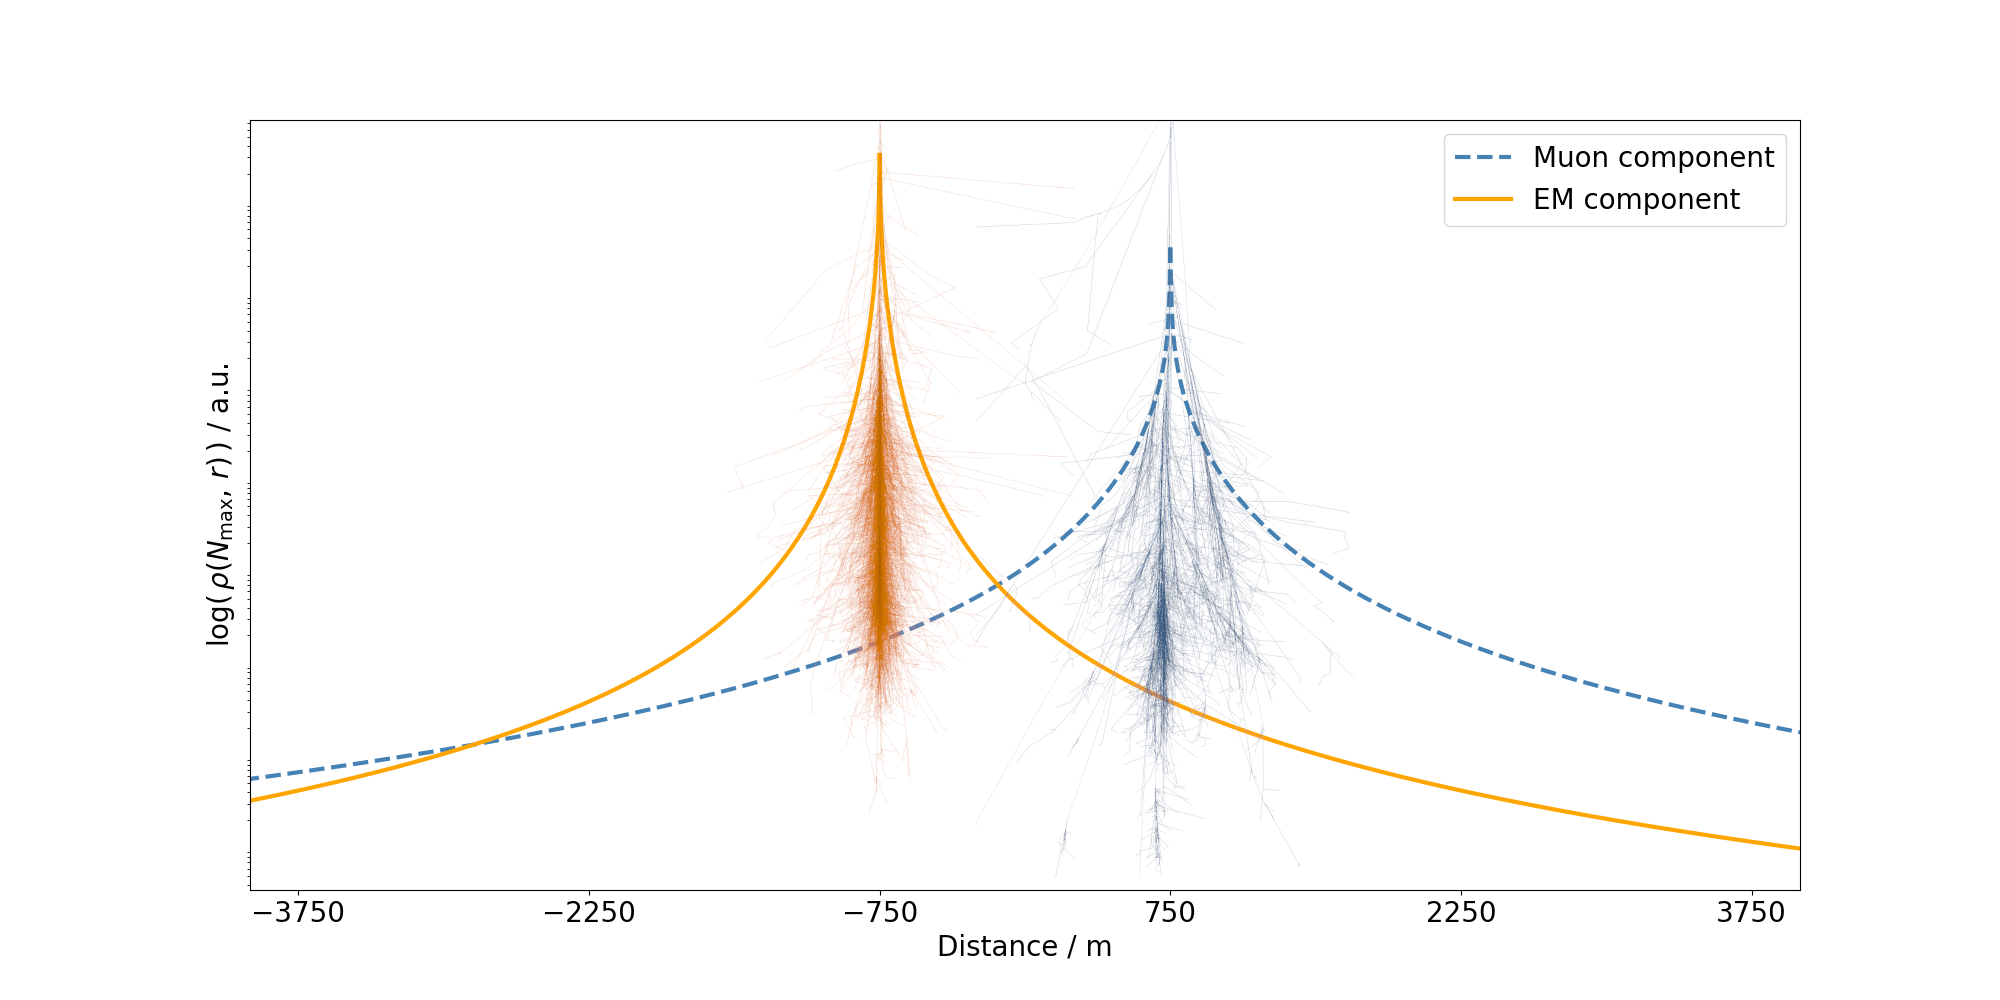
\includegraphics[width=1.0\textwidth]{./plots/componentwise_LDF.png}
	\caption{The lateral distribution function for the muonic (steelblue) and electromagnetic (orange) component of a vertical, \SI{100}{\giga\electronvolt}
	proton shower at roughly sea level ($r_\text{M}=\SI{100}{\meter}$). The inset plots on the top-right represent the xz-projection of the shower shape. Both 
	images adopted with changes from \cite{CorsikaShower}.}
	\label{fig:component-LDF}
\end{figure}

\section{Composite primaries}
\label{sec:superposition-principle}

As is evident from the discussion in \autoref{chap:physical-background}, not only single protons (which are strictly speaking also composite) or elementary 
particles like photons, electrons, etc. appear in the cosmic ray spectrum. Any and all kind of elements can and do appear as possible primaries, given that they
are stable to weak decay and can be effectively accelerated near a CR source. The consequence of different primaries on resulting shower characteristics is subtle,
but large enough such that it can be used for identification purposes.

Assuming the constituents in a CR nucleus all coherently interact with an air molecule, one arrives at the superposition principle for extensive air showers. It 
states that for a composite primary with $A = N + Z$ neutrons and protons, each constituent particle will initiate a shower with initial energy of 
$E_0' = E_0\,/\,A$, where $E_0$ is the initial energy of the composite particle. It follows that air showers from heaver primaries occur at higher altitudes (lower 
atmospheric depth $X$) and with higher particle counts.

\begin{equation}
N_{\text{max},\,A} = A \cdot N_{\text{max},\,1}, \qquad n_{\text{max},\,A} = \left\lfloor \log_N\left(\frac{E_0}{E_{c,\,\text{had}}}\right) - \log_N A \right\rfloor,
\end{equation}

where $N_{\text{max},\,1}$ refers to a proton shower as established in \autoref{eq:n-max-matthews}.

\section{Comments on validity}
\label{sec:cr-shower-validity}

The Heitler model and Heitler-Matthews model discussed in \autoref{sec:heitler-model} and \autoref{sec:heitler-matthews-model} respectively make only very 
rudimentary assumptions on the underlaying physics of particle cascades. Nevertheless, the equations recovered from these assumptions are already a close 
approximation of real world processes up to $X_\text{max}$. 

Of course, adding a stochastic component to the above assumptions (c.f. \cite{MartinShowerSim}) improves predictions. But even full-fledged Monte-Carlo simulation 
software frameworks like GEANT4 \cite{agostinelli2003geant4} or CORSIKA \cite{heck1998corsika} show discrepancies between observed and predicted shower development. 
An example of this is presented in \autoref{fig:model-validity}. 

While shower-to-shower fluctuations can explain discrepancies to a degree, there also exist systematic differences between the simulated and observed extensive air
showers. These are largely owed to imprecise knowledge of the underlaying physical processes. For example, hadronic interaction models (e.g. QGSJETII-04 shown in 
\autoref{fig:validity-plot}) rely on extrapolation of measured cross sections in the \SI{}{\giga\electronvolt}-\SI{}{\tera\electronvolt} scales to the relevant 
CR energies \cite{ostapchenko2006qgsjet}. While this is not an unfair assumption given the scale invariance of deep inelastic scattering \cite{fox1974early}, it is 
clear, that the approach cannot accurately encompass all effects that may take place at high energies.

In conclusion, the particle cascades evolving from relativistic CRs impinging on earth are still not fully understood. Several simulation frameworks have been 
developed, which each have their own shortcomings. It is therefore important to compare not only results from simulations using one framework to observations, but 
also different simulations with each other.

\begin{figure}
	\centering
	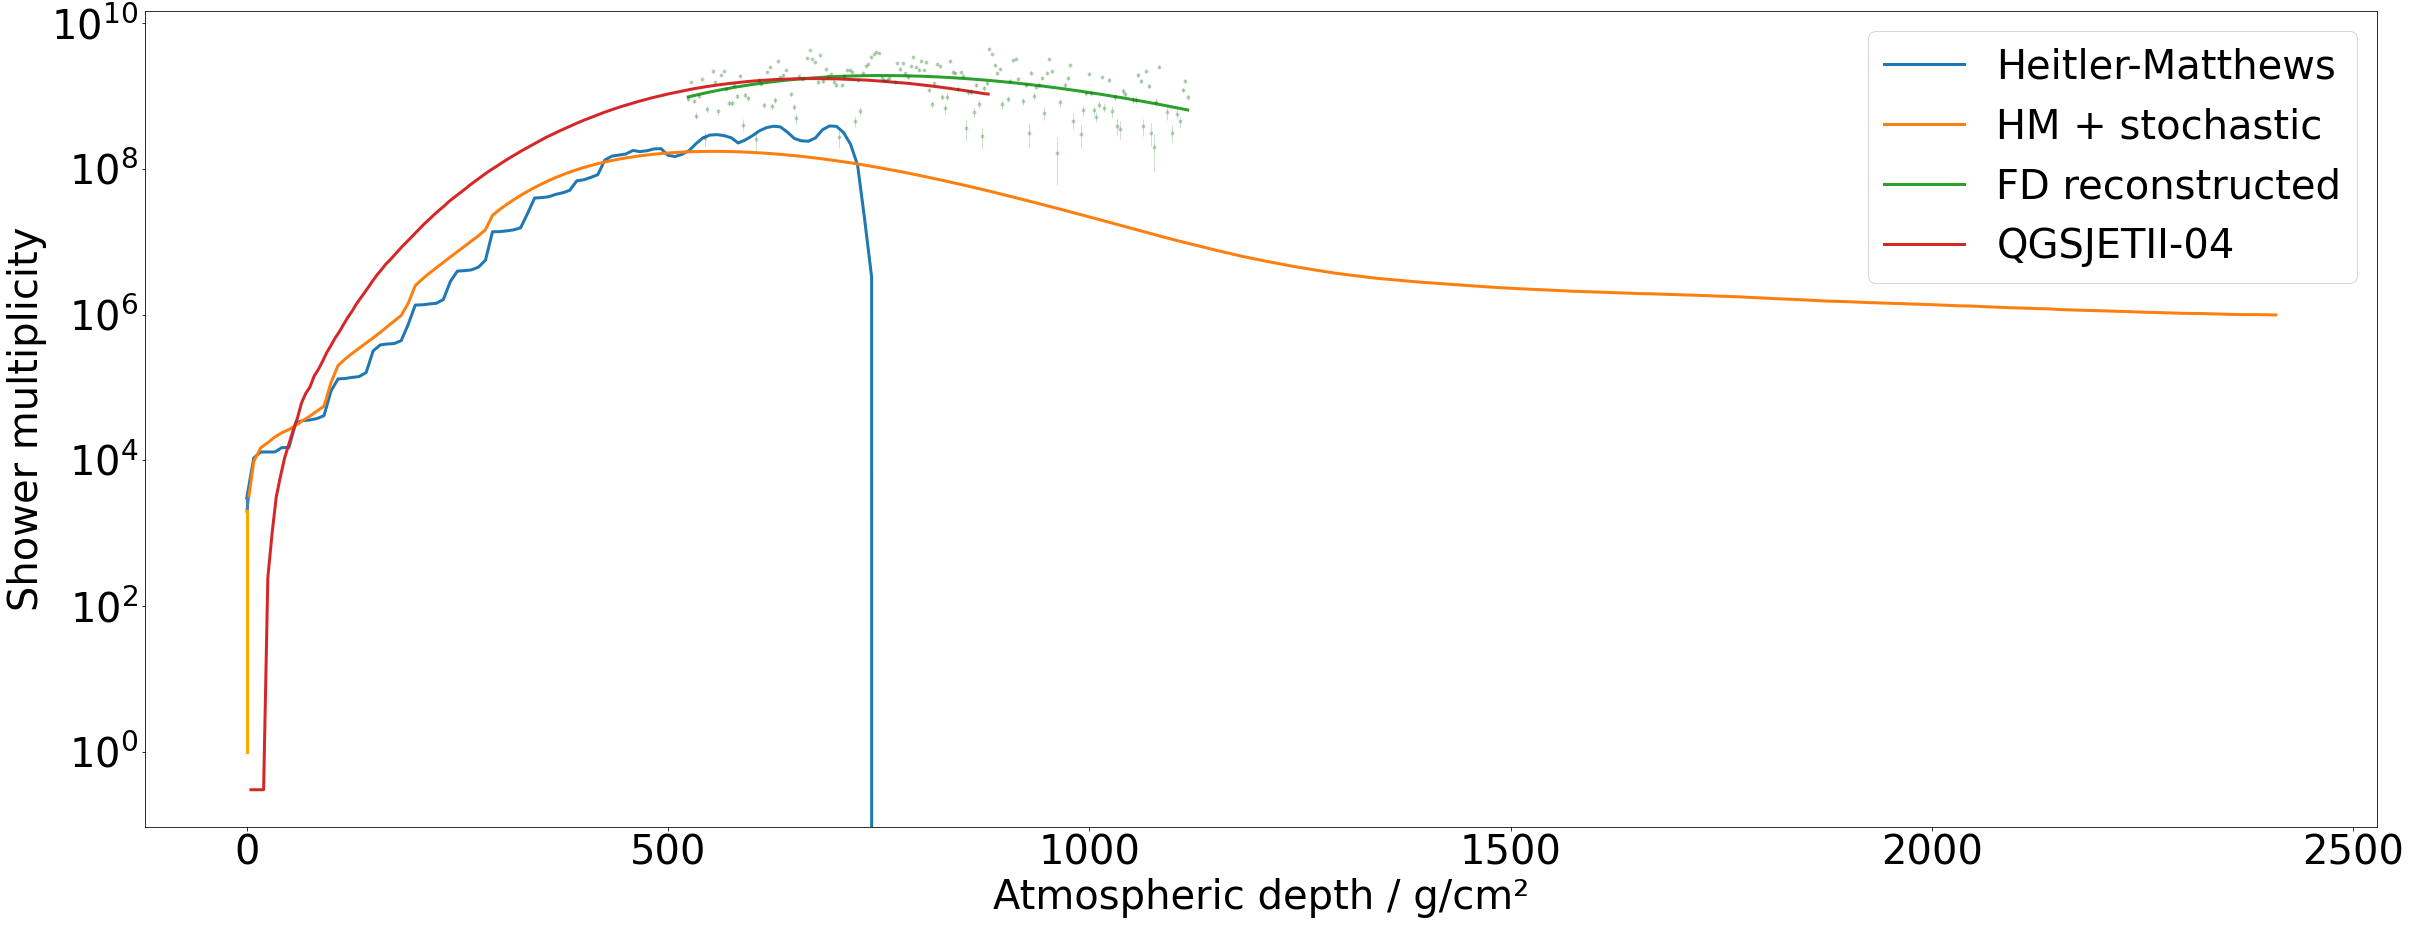
\includegraphics[width=1.0\textwidth]{./plots/validity_plot.png}
	\caption{Comparison of the number of charged particles for different physics models to reconstructed observations from a $~\SI{3}{\exa\electronvolt}$ proton 
	shower. Shown in steelblue and orange is the Heitler-Matthews model as described in \autoref{sec:heitler-matthews-model}, and extended with a stochastic 
	component. An example of a more in-depth simulation in red, and observed shower multiplicities in green.}
	\label{fig:model-validity}
\end{figure}

\section{Detection methods}
\label{sec:detection-methods}

\subsection{Fluoresence}
\label{ssec:fluoresence}

\subsubsection{In Air}


\subsubsection{In Scintillators}


\subsection{Cherenkov light}
\label{ssec:cherenkov-light}

When a charged particle exceeds the phase velocity of light in a medium with refractive index $n$, the optical equivalent of a sonic boom occurs. Photons travel in a 
shockwave along an angle $\theta = \arccos\left(n^{-1}\beta^{-1}\right)$ relative to the trajectory of the particle while $\beta \geq \frac{c}{n}$. This process is 
well understood and can be used to detect high energy cosmic rays.

\subsubsection{In Air}

The refractive index of air ranges from 1 in the near vacuum of the upper atmosphere to $\approx1+2.9\cdot10^{-4}$ at sea level \cite{andrews1992analytical}. This
implies that only particles with a Lorentz factor $\gamma \gtrsim 41.5$ emit Cherenkov light, which is satisfied for e.g. muons and protons already in the low
\SI{}{\giga\electronvolt} ranges.

It can therefore be expected that extensive air showers, that contain high energy charged particles, produce considerable amounts of Cherenkov light. With a 
sensitive enough telescope, or telescope array, this light, and by extension the air shower can be detected. The \textbf{C}herenkov \textbf{T}elescope 
\textbf{A}rray (CTA) utilizes this measurement technique and is due to commence operations in 2024 \cite{actis2011design}.

\subsubsection{In Water}



\subsection{Radio Emission}
\label{ssec:radio-emission}
	% %! TEX root = ../thesis.tex

\chapter{The Pierre Auger Observatory}
\label{chap:auger-observatory}

Located on the argentinian high-plains of Pampa Amarilla, the Pierre Auger observatory is a hybrid detector designed to detect and study cosmic rays of the highest
energies. With an effective area of \SI{3000}{\kilo\meter\squared} it is by far the largest experiment of its kind \cite{DesignReport}.

Altough first proposed in 1992, it took 18 years until the idea of a large scale experiment to detect cosmic rays matured and construction of the first prototype 
started near Mendoza \cite{AugerTimeline}. Some further 20 years later, the Pierre Auger collaboration has published over 110 papers \cite{PCollab} and continues to 
advance research in astroparticle physics.

It does this via a hybrid approach, combining measurements of a \textbf{S}urface \textbf{D}etector (SD) as well as a \textbf{F}louresence \textbf{D}etector (FD). 
Additional machinery, such as the e\textbf{X}treme (XLF) and \textbf{C}entral \textbf{L}aser \textbf{F}acility (CLF), is installed to monitor atmospheric 
variables. This improves the overall systematic accuracy of predictions made by the experiment. An overview of the site can be seen in \autoref{fig:auger-array}. 
Data measured by the FD, SD and the atmospheric monitors is sent to a \textbf{C}entral \textbf{D}ata \textbf{A}cquisition \textbf{S}ystem (CDAS) located in the 
nearby town of Malargüe.

This chapter offers a brief look into the measurement principle and setup of the observatory. Information regarding the fluoresence detector can be found in 
\autoref{sec:fluoresence-detector}. The SD is described in \autoref{sec:surface-detector}. A more in depth read on detector specifications and design choices is 
represented by the Pierre Auger observatory design report \cite{DesignReport}, where a lot of information stated in this chapter is conglomerated from. Notes on 
the event reconstruction are listed in \autoref{sec:event-reconstruction} and summarized from \cite{SDReconstruction} and \cite{FDReconstruction}.

\begin{figure}
	\centering
	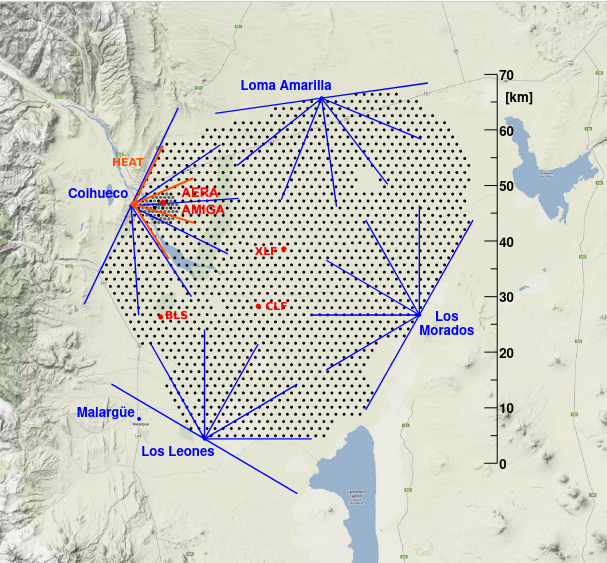
\includegraphics[width=0.9\textwidth]{imgs/auger_array.png}
	\caption{Overview of the Pierre Auger observatory. The four different FD sites (respective FOV shown with blue lines) sit at the edge of the detector area and 
	monitor the night sky above the SD array consisting of 1600 water tanks (black dots). A denser spacing of stations near Coihueco is equipped with additional 
	electronics such as e.g. radio antennas (AERA) and muon detectors (AMIGA). Image taken from \cite{AugerArray}}. \label{fig:auger-array}
\end{figure}

\begin{figure}
	\begin{subfigure}[b]{0.5\textwidth}
		\centering
		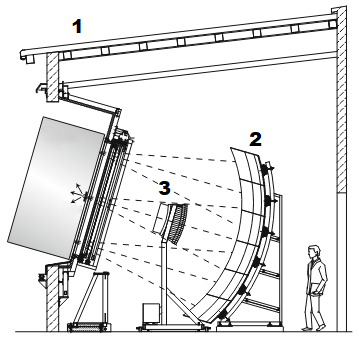
\includegraphics[width=\textwidth]{./imgs/auger_fd.png}
		\caption{\textbf{FD eye setup}}
		\label{fig:fd-eye}
	\end{subfigure}
	\hfill
	\begin{subfigure}[b]{0.5\textwidth}
		\centering
		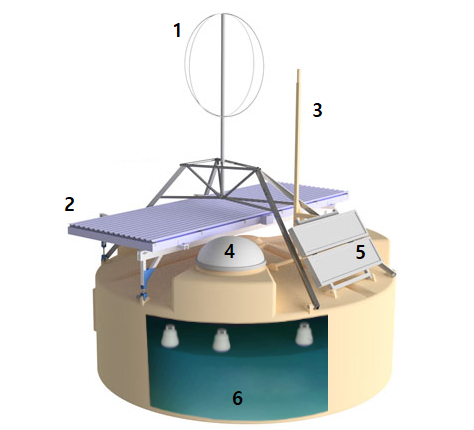
\includegraphics[width=\textwidth]{./imgs/auger_sd.png}
		\caption{\textbf{SD station setup}}
		\label{fig:sd-station}
	\end{subfigure}
	\caption{\textbf{(a)} Schematic view of an FD eye with housing (1), main mirror (2) and camera (3). Image taken from \cite{FDReconstruction} \textbf{(b)} Setup
	of an SD WCD with radio antenna (1), SSD (2), communication and GPS antenna (3), electronics box (4), solar panesl (5) and the WCD (6). Image adopted with 
	changes from \cite{UUBstation} and \cite{waterTank}}
\end{figure}


\section{Fluoresence Detector (FD)}
\label{sec:fluoresence-detector}

The FD consists of a total of 27 fluoresence telescopes (eyes) at 4 different sites. Each eye monitors a \SI{30}{\degree} x \SI{30}{\degree} window of the sky at a
resolution of $\approx \, 0.5 \, \frac{ \text{px} }{ \text{deg}^2 }$. This results in an effective FOV of roughly \SI{180}{\degree} x \SI{30}{\degree} per FD 
station, with an exception of Coihueco, where three additional telescopes - HEAT (\textbf{H}igh \textbf{E}levation \textbf{A}uger \textbf{T}elescope) - are 
installed to enable monitoring of higher zenith angles ($\SI{30}{\degree}\leq\theta\leq\SI{60}{\degree}$) and increase sensitivity for showers of lower energies 
(compare \autoref{chap:physical-background}). A schematic of the setup of each eye is given in \autoref{fig:fd-eye}.

The individual telescopes consist of \SI{3.6}{\meter} by \SI{3.6}{\meter}, convex mirrors. They reflect incoming light onto a set of 440 photomultipliers (PMTs), 
each corresponding to one pixel in the resulting image seen by an eye. Since the setup needs to be extremely sensitive to UV light in order to detect flouresence 
caused by extensive air showers, its operation is limited to the relatively noise free moonless astronomical nights (Sun $\measuredangle$ Horizon 
$\lesssim-18^{\circ}$). When the FD is operational, this allows the observation of the longitudinal propagation of a shower instead of just its' footprint (as seen 
by the SD). 

\section{Surface Detector (SD)}
\label{sec:surface-detector}

The SD consists of 1600 individually operating stations, spaced apart on a hexagonal grid with a standard \SI{1.5}{\kilo\meter} spacing. Each 
station is made up of a main tank filled with \SI{12000}{\litre} of purified water and reflective inner walls, a solar panel and batteries for power management, 
as well as an antenna for communication. Within each tank three PMTs detect Cherenkov light originating from shower particles, these are together with the tank 
referred to as \textbf{W}ater \textbf{C}herenkov \textbf{D}etectors (WCDs). With the (at the time of this work) ongoing AugerPrime upgrade, each station is 
additionally equipped with a \textbf{s}mall \textbf{PMT} (sPMT), \textbf{S}urface \textbf{S}cintillator \textbf{D}etector (SSD), and radio antenna atop the tank.
This allows for the recording of stronger signals, finer separation of electromagnetic and muonic shower component and detection of highly inclined air showers 
respectively \cite{AugerPrime, horandel2019precision}. \autoref{fig:sd-station} shows a schematic blueprint of each SD station.

\subsection{Data acquisition (DAQ)}
\label{ssec:sd-daq}

Onboard electronics, the \textbf{U}pgraded \textbf{U}nified \textbf{B}oard (UUB), or more precisely six 10-bit \textbf{F}lash 
\textbf{A}nalog-to-\textbf{D}igital-\textbf{C}onverters (FADCs) read out measurement data from the PMTs at a sampling rate of \SI{120}{\mega\hertz} 
($\approx\SI{8.33}{\nano\second}$ binning) \cite{verzi2013energy}. This is done in a two-fold way. Three FADCs digitize the PMTs dynode voltage, resulting in the
\textbf{H}igh \textbf{G}ain (HG) output. Three FADCs monitor the anode voltage to form the \textbf{L}ow \textbf{G}ain (LG) output, which can be analyzed if the 
HG output exceeds a value of $2^{10}$ ADC counts and becomes saturated. This effectively enables the measurement of both large ($\geq\mathcal{O}(10^3)$ particles
hitting the tank) as well as small shower signals ($\mathcal{O}(1)$ particle hitting the tank) with sufficient accuracy \cite{SDReconstruction}. Once an FADC bin 
has been recorded and checked for possible triggers (c.f. \autoref{chap:classical-triggers}) via \textbf{F}ield \textbf{P}rogrammable \textbf{G}ate 
\textbf{A}rrays (FPGAs) it is written to a ring buffer. If a trigger is issued, the corresponding chunk in the ring buffer ($\approx\SI{4.992}{\micro\second}$ 
(599 bins) before and $\SI{12.07}{\micro\second}$ (1448 bins) after a trigger, $2047 + 1$ bins total), the measured trace, can be analyzed in order to calibrate a 
station in the array (\autoref{ssec:online-calibration}, \autoref{ssec:offline-calibration}) or processed by a higher-level CPU for event reconstruction purposes 
(see \autoref{sec:event-reconstruction}).

While each station is equipped with the same electronics and runs the same analysis software, variables like the position in the field, station age or slight 
changes in the manufacturing/installation process cause different stations to age differently. Over the lifetime of the array such differences can sum into 
potentially drastic discrepancies in gathered data. Put simply, an extensive air shower will look different both to different WCDs at the same time as well as 
the same WCD at different times. To account for this, measurements are standardized across all stations. ADC counts are related to a \textbf{V}ertical 
\textbf{E}quivalent of through-going \textbf{M}uons (VEM) that would result in the same signal strength. In this fashion, the maximum response that is generated 
by a PMT from one vertically through-going muon is defined as \SI{1}{\Peak}. The total deposited charge (equivalent to the integral of the response) is defined 
as \SI{1}{\Charge}. The conversion factor between ADC counts and VEM$_\text{Peak}$ and VEM$_\text{Ch.}$ (referred to as \Ipeak and \Qpeak respectively) is 
estimated from data and continuously updated separately for each station. Note that due to the limited computational resources of the WCD, as well as constraints
on the amount of data that can be transmitted per station in the SD array (\SI{1200}{\bit\per\second}, \cite{localStationCalib}), a simplified, rate-based approach 
is implemented for autonomous calibration in the field (Online calibration), this stands in contrast to the more physics-driven histogram method used during event 
reconstruction via the official Auger reconstruction and simulation framework, \Offline \cite{offlineSource}. In any case, both algorithms are listed in the 
following subsections and 
discussed in more detail in the referenced literature.

\subsection{\Offline calibration}
\label{ssec:offline-calibration}

\subsubsection{Baseline estimation}
\label{sssec:offline-baseline-estimation}

In order to estimate \Ipeak and \Qpeak of a WCD tank first the baseline - the average response in the absence of any signals - of each PMT needs to be determined. 
All further analysis will then be based on the baseline-subtracted PMT data.

For event reconstruction, a first baseline estimate of a WCD PMT is predicted by examining the beginning and end of a 2048 bin ($\SI{17.06}{\micro\second}$) long 
trace. The mode $m$ as well as standard deviation $\sigma$ of the first (last) 300 bins is calculated. All bins larger or smaller than $m\pm2\sigma$ are truncated 
and removed from the trace window. The value of $m$, $\sigma$ is consequently updated and the procedure repeated until a convergence is reached and no further cut 
is necessary. The best estimate $B_\text{front}$ ($B_\text{end}$) for the front (end) of the trace at this point is given by the mean value of all remaining bins. 
It's statistic uncertainty $\sigma_{B_\text{front}}$ ($\sigma_{B_\text{end}}$) is given by the standard deviation of the remaining bins \cite{tobiasBaseline}. The 
baseline between the flat front and end estimate is then interpolated based on the difference 

\begin{equation}
	\Delta B = B_\text{end} - B_\text{front}.
\end{equation}

\begin{itemize}
	\item \textbf{Rejection of anomalous upward fluctuations} $\mathbf{\frac{\Delta B}{\sigma_{\Delta B}} \geq +10}$:

	$B_\text{end}$ being higher than $B_\text{front}$ often indicates errors in the electronic readout or defect components in the measurement chain. There 
	exists no physical reason why the end baseline should be (significantly) higher than the front. Consequently, traces where this is the case are ignored 
	during event reconstruction.

	\item \textbf{Constant approximation for small upward fluctuations} $\mathbf{+5 > \frac{\Delta B}{\sigma_{\Delta B}} \geq 0}$:

	Small fluctuations of the baseline are expected and the norm. If these fluctuations are positive ($B_\text{end} > B_\text{front}$) the method of 
	calculating the mode, truncating outliers and repeating both steps is applied to the entire length of the signal, resulting in a constant baseline estimate
	$B$ across the trace.

	\item \textbf{Step-function approximation for small downward fluctuations} $\mathbf{0 > \frac{\Delta B}{\sigma_{\Delta B}} \geq -1}$:

	Unlike positive fluctuations, negative fluctuations ($B_\text{end} < B_\text{front}$) can have a physical significance. Due to the undershoof of PMTs after
	detecting a signal in the WCD (compare \cite{glietta2008recovery}), the baseline estimate decreasing towards the end of the trace often indicates the 
	presence of shower particles within the tank. For this reason, downward fluctuations are handled differently from upward ones. If the fluctuations are 
	sufficiently small, the baseline across the trace is estimated as a simple step-function; The trace is separated into two parts along its' maximum ADC 
	value. The front part (i.e. before the max. value) has the baseline $B_\text{front}$, while the rear part is estimated by $B_\text{end}$. An example of 
	this is shown in \autoref{fig:baseline-step-function-approximation}.

	\item \textbf{Charge-linear approximation for large undershoots} $\mathbf{-1 \geq \frac{\Delta B}{\sigma_{\Delta B}}}$:

	For larger undershoots, the baseline is estimated bin by bin based on the deposited charge in the detector. Starting with a value of $B_\text{front}$ for 
	the bins 1-300, the remaining baseline is first linearly interpolated according to \autoref{eq:baseline-charge-linear-interpolation},

	\begin{equation}
	\label{eq:baseline-charge-linear-interpolation}
		b_i = B_\text{front} - \Delta B \cdot \frac{i - 300}{1448}, \qquad 300 \geq i \geq 2048,
	\end{equation}	

	where the magic numbers 300 and 1448 refer to the last bin of the front baseline estimate and the length of the interpolated baseline respectively. From 
	this, the deposited charge $q_i$ up to bin $i$ can be calculated as per \autoref{eq:deposited-charge}.

	\begin{equation}
	\label{eq:deposited-charge}
		q_i = \sum_{k = 0}^{i} \left( T_k - b_k \right)\exp\left(-\frac{\SI{8.33}{\nano\second}}{\tau}\cdot(i-k)\right)
	\end{equation}
	
	In \autoref{eq:deposited-charge}, $T_k$ refers to the numerical value of bin $k$. Note that an exponential falloff term has to be added to account for the
	decay in signal undershoot with a decay time of $\tau = \SI{45}{\micro\second}$. The value of $\tau$ is determined in \cite{tobiasBaselineUUB}. Assuming 
	the magnitude of the signal undershoot is directly proportional to the deposited charge $q$, a correction of the baseline thus becomes

	\begin{equation}
	\label{eq:baseline-correction}
		b_i = B_\text{front} + \frac{q_i}{q_{1898}} \cdot \Delta B.
	\end{equation}
	
	The parametrization in \autoref{eq:baseline-correction} is chosen such that the charge-interpolated baseline at bin $1898$ (the center position in the last
	$300$ bins) is exactly equal to the rear baseline estimate $B_\text{end}$. The prediction can be made more accurate by repeating the above steps, each time
	recalculating $q_i$ and readjusting the baseline $b_i$ in the process. \autoref{fig:baseline-charge-linear-interpolation} shows an example baseline 
	estimate after three such iterations. In general, it converges to a robust estimate within five repetitions \cite{tobiasBaselineUUB}.

\end{itemize}

\begin{figure}
	\begin{subfigure}[b]{0.5\textwidth}
		\centering
		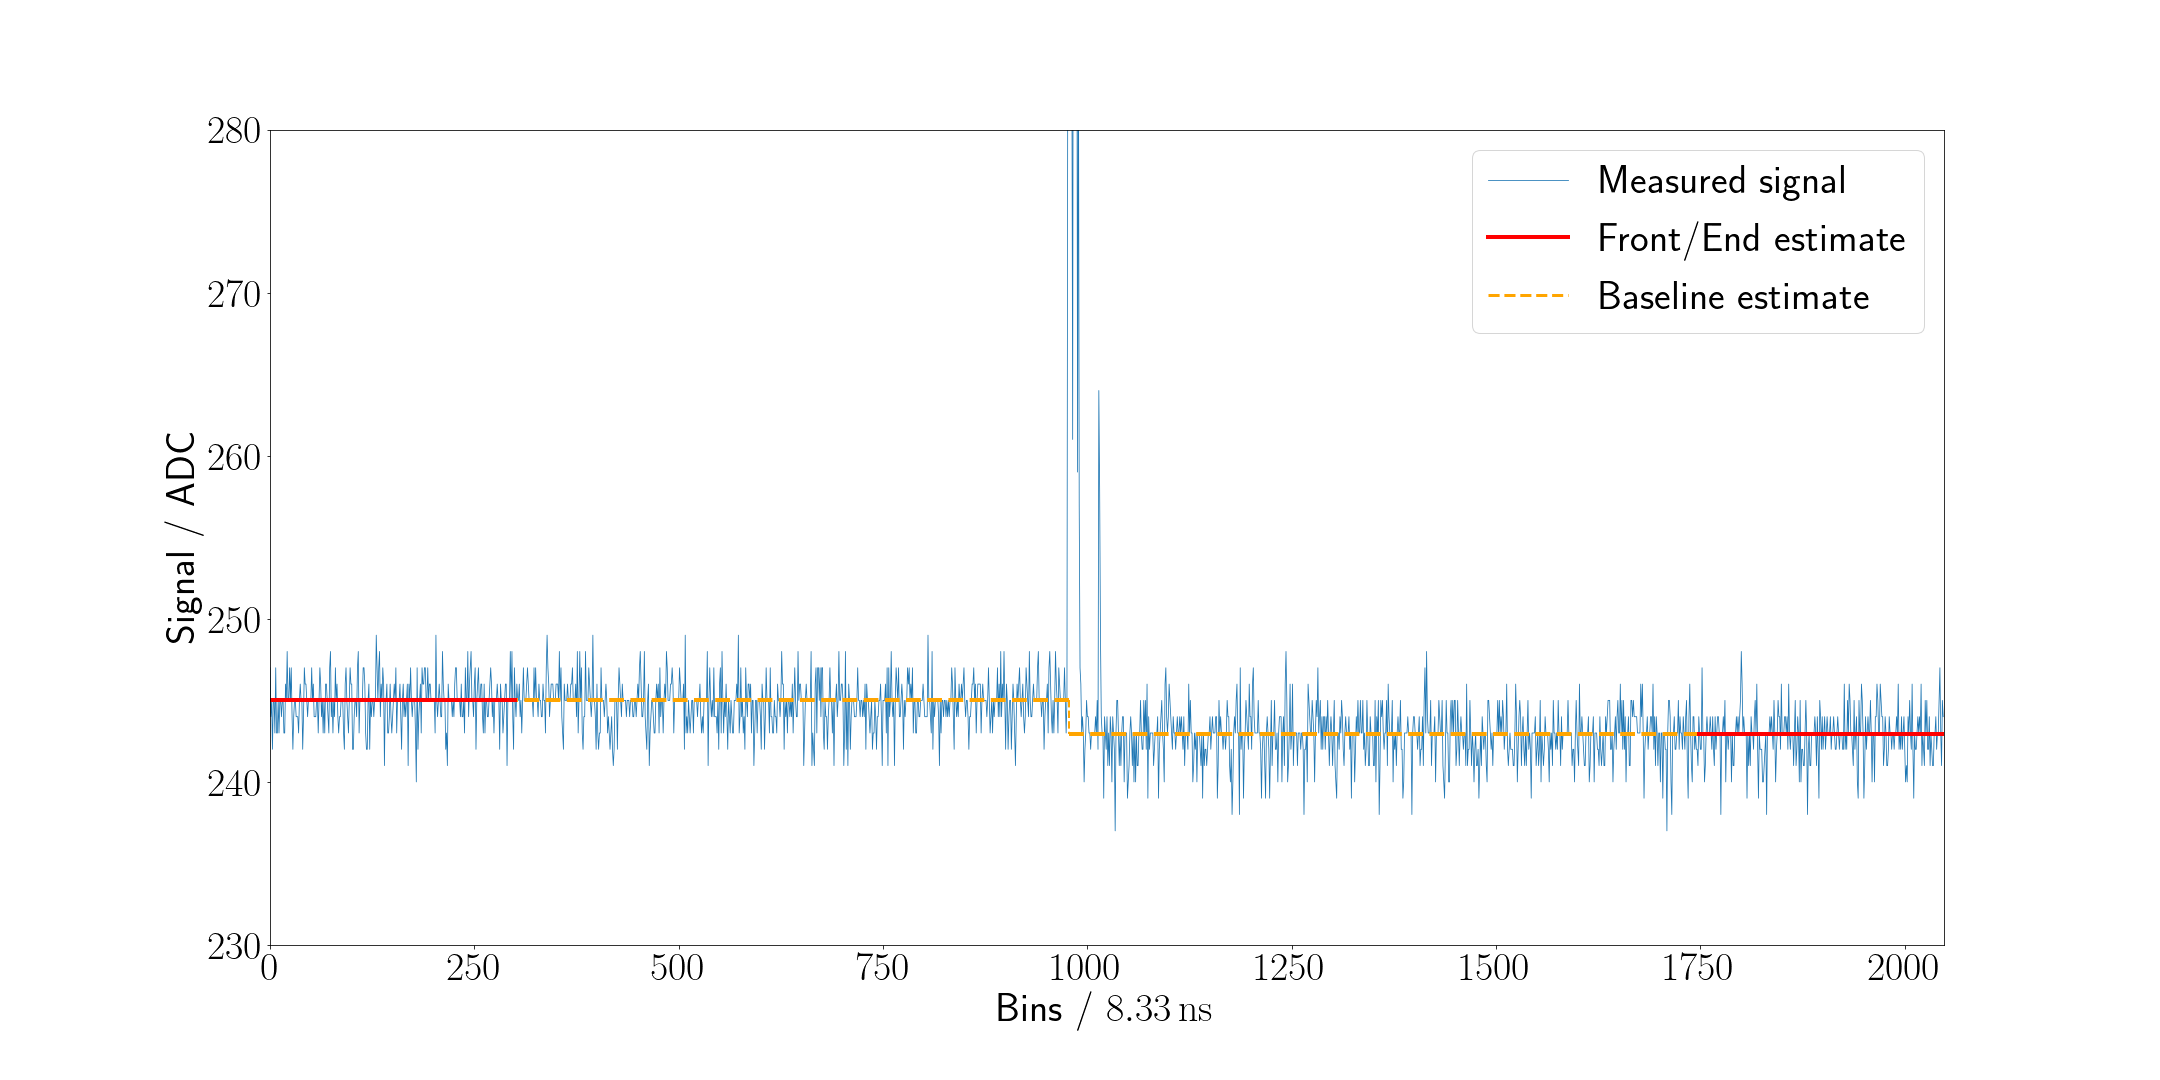
\includegraphics[width=\textwidth]{./plots/baseline_step_function.png}
		\caption{\textbf{Step-function approximation}}
		\label{fig:baseline-step-function-approximation}
	\end{subfigure}
	\hfill
	\begin{subfigure}[b]{0.5\textwidth}
		\centering
		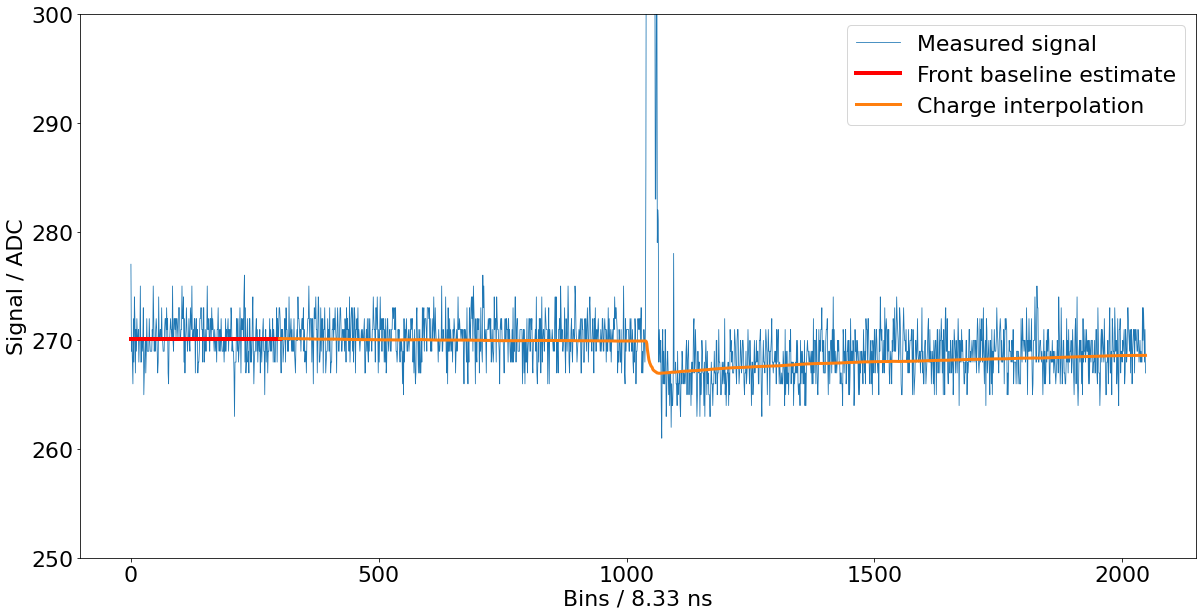
\includegraphics[width=\textwidth]{./plots/baseline_charge_interpolation.png}
		\caption{\textbf{Charge-linear interpolation}}
		\label{fig:baseline-charge-linear-interpolation}
	\end{subfigure}
	\caption{\textbf{(a)} A simple step function is	sufficient to accurately model a PMTs' noise level at small downward fluctuations. \textbf{(b)} For larger 
	discrepancies the more involved charge-linear interpolation is used. Note that the signal undershoot is exaggerated for visualization purposes in both 
	examples.}
\end{figure}

\subsubsection{Estimation of \Ipeak and \Qpeak}
\label{sssec:offline-vem-calibration}

The conversion factor between ADC counts and VEM$_\text{Peak}$, VEM$_\text{Ch.}$ are built from distributions of traces that satisfy the muon trigger, which scans
incoming ADC bins for a value exceeding the muon threshold $t_\upmu = b + \SI{30}{\ADC}$, \SI{30}{\ADC} above baseline, for any of the three WCD PMTs. If this 
requirement is met, 69 bins (19 before, trigger bin, 49 after) are written to the muon buffer, a FIFO (first-in-first-out) type memory storage, that is
subsequently filled with low-energy events, which (in general) didn't satisfy any other trigger but still contain useful information \cite{localStationCalib}.

By histogramming the maximum value (sum) of each trace, the plot shown in \autoref{fig:offline-vem-peak} (\autoref{fig:offline-vem-charge}) can be obtained. It 
becomes apparent that the number of events per bin largely follows a power law with negative spectral index. This is expected considering the discussion in 
\autoref{chap:physical-background}. Noteable are characteristic deviations from this powerlaw, as these contain information about \Ipeak and \Qpeak:

\begin{itemize}
	\item Low energy events from e.g. $e^-$, $e^+$ that deposit their entire energy in the tank give rise to a surplus of events at lower ADC values.
	\item A characteristic (muon) hump appears in the bins $20 - 70$. This surplus is caused by omni-directional muons impinging onto the detector. Since the 
	energy deposited by such muons is roughly constant, the center of the muon hump serves as an estimate of \Ipeak (\Qpeak).
	\item (Not depicted in \autoref{fig:offline-calibration}) In similar plots from related works (c.f. \cite{localStationCalib, streich2018performance}) a
	drastic increase in bin occupations towards the tail end of the histograms can be observed. This is attributed to an increased bin size from \SI{1500}{\ADC} 
	counts onwards, which reduces the amount of data per station sent to CDAS. In the example plots referenced here, a constant binning is chosen instead. 
	This difference is mentioned here to avoid possible confusion. 
\end{itemize}

In this fashion, the average response of the WCD to a through-going muon can be estimated by e.g. fitting a gaussian distribution to the muon hump. However, 
there exists a systematic difference between the response to a vertical or an omni-directional muon. Consequently, correctional factors need to be applied to the 
analysis results. These have been determined in previous experiments \cite{allison2002surface}. Finally, one arrives at an estimate for the conversion factor 
between ADC counts and VEM$_\text{Peak}$, VEM$_\text{Ch.}$.

\begin{figure}
	\begin{subfigure}[b]{0.5\textwidth}
		\centering
		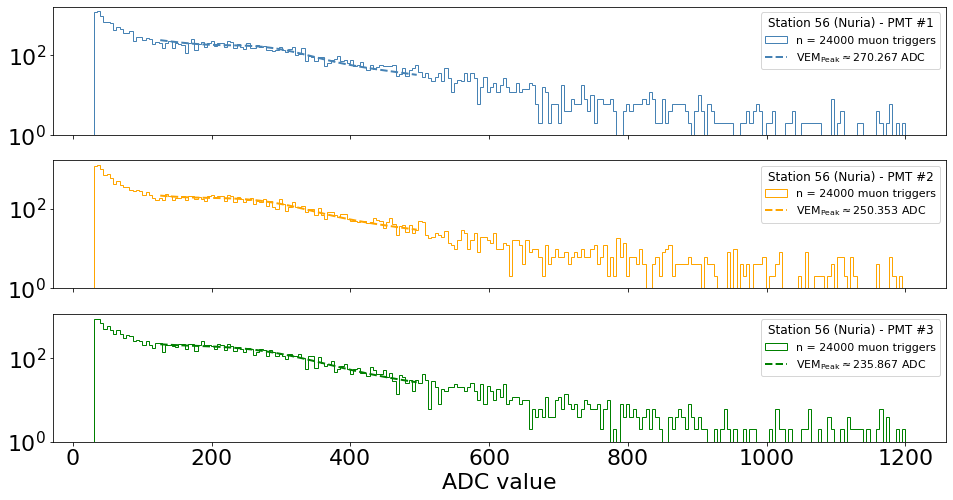
\includegraphics[width=\textwidth]{./plots/offline_vem_peak.png}
		\caption{\textbf{VEM}$_\textbf{Peak}$ \textbf{Histogram}}
		\label{fig:offline-vem-peak}
	\end{subfigure}
	\hfill
	\begin{subfigure}[b]{0.5\textwidth}
		\centering
		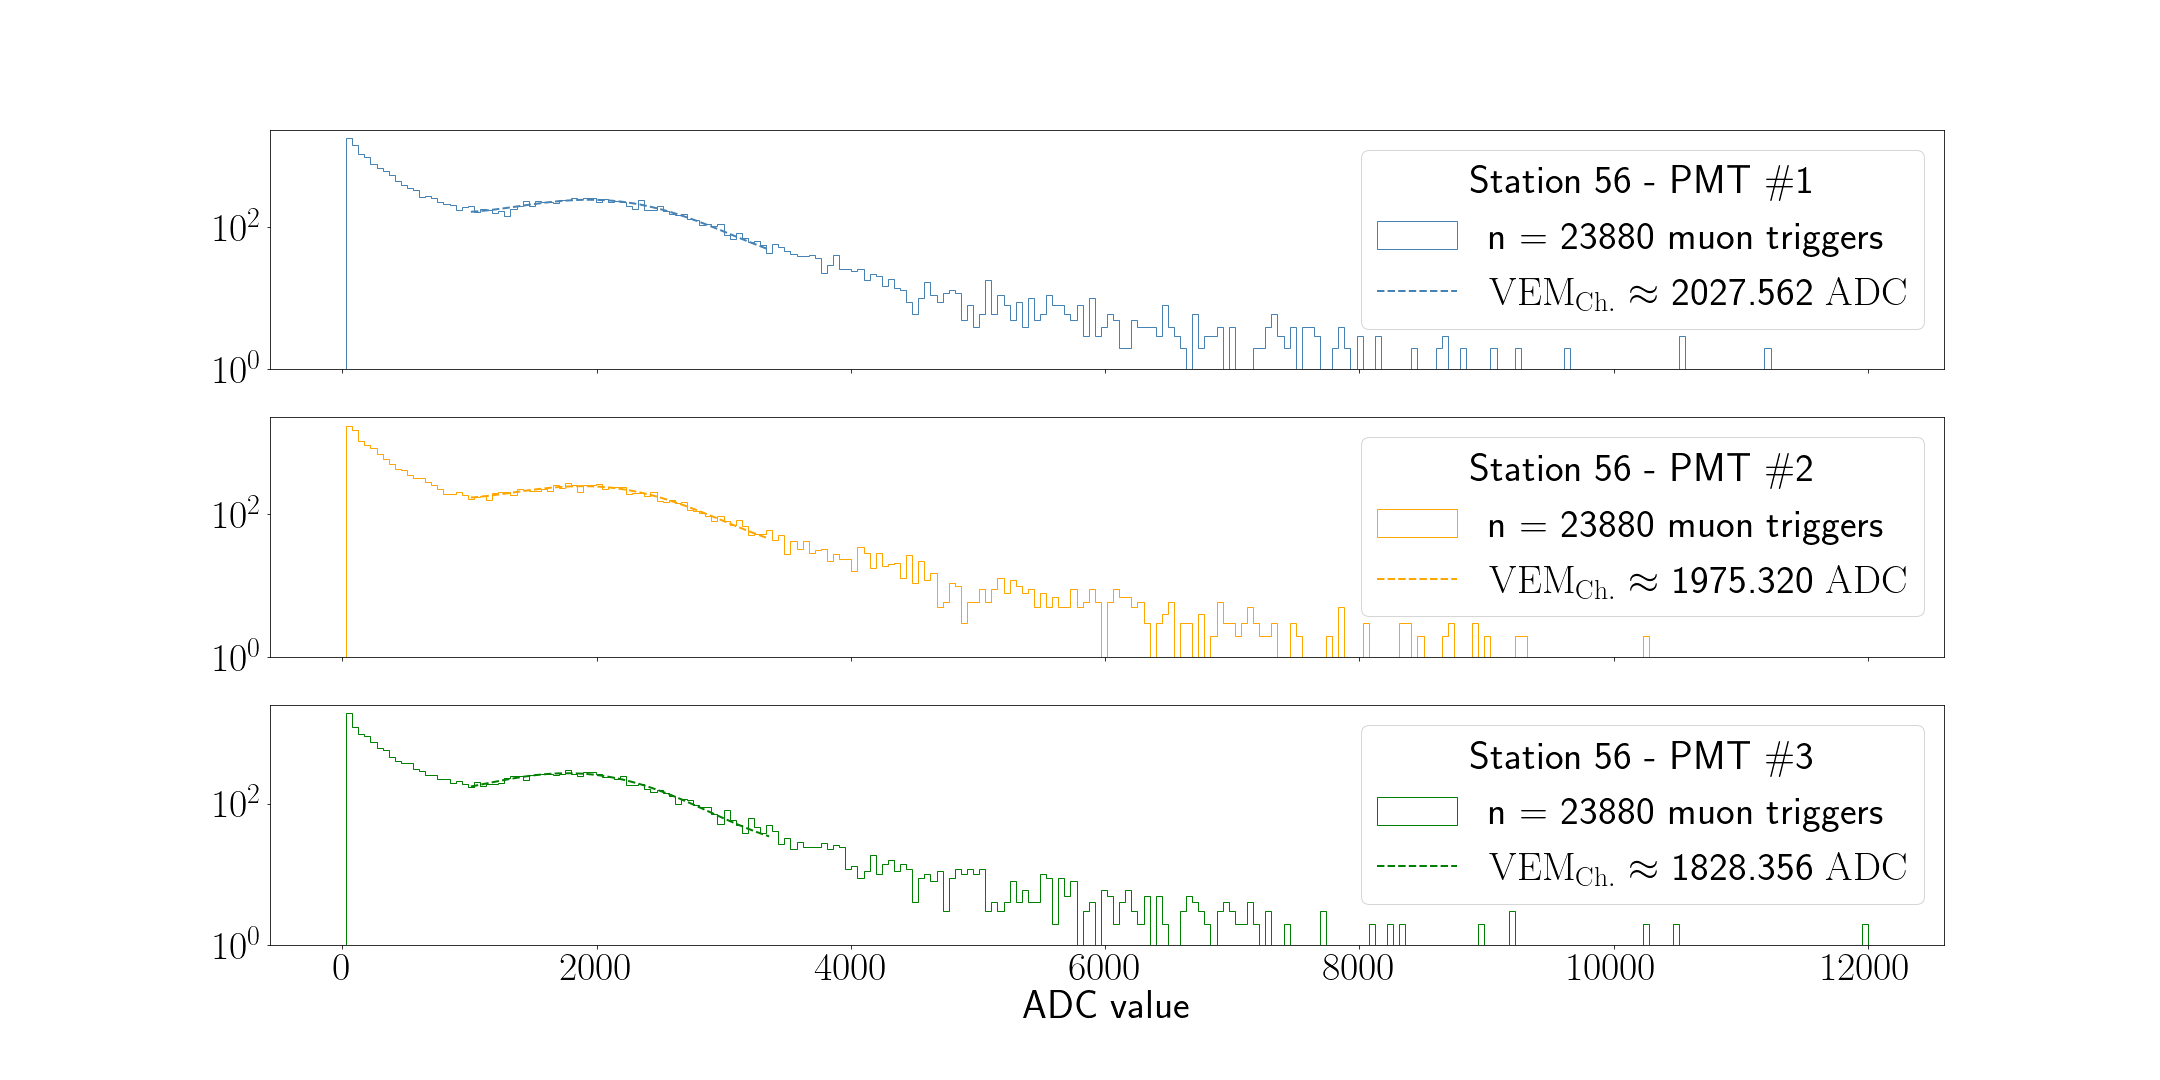
\includegraphics[width=\textwidth]{./plots/offline_vem_charge.png}
		\caption{\textbf{VEM}$_\textbf{Ch.}$ \textbf{Histogram}}
		\label{fig:offline-vem-charge}
	\end{subfigure}
	\caption{\textbf{(a)} The maximum value of each muon trace is histogrammed in order to gain information about the current value of \Ipeak of a station. 
	\textbf{(b)} The conversion factor from recorded ADC values to \Qpeak is given from the histogrammed sum of each muon trace.}
	\label{fig:offline-calibration}
\end{figure}

\subsection{Online calibration}
\label{ssec:online-calibration}

\subsubsection{Baseline estimation}
\label{sssec:online-baseline-estimation}

Each SD station has an autonomous estimate of its' three WCD PMT baselines. They are defined simply as the mean of all first bins for each trace contained in the 
respective muon buffers (see \autoref{sssec:offline-vem-calibration}). This baseline estimate is used to set the thresholds of the hardware triggers discussed in 
\autoref{chap:classical-triggers}.

\subsubsection{Estimation of \Ipeak and \Qpeak}
\label{sssec:offline-vem-calibration}

Due to the limited computational resources in each station, the determination of \Ipeak and \Qpeak at station-level is fairly naive. Nevertheless, the 
$\sigma$-$\delta$-method shown here has proven to be incredibly robust over the lifetime of the SD array \cite{DesignReport}. 

In the beginning, the to-be-estimated value $I_\text{Peak}^\text{est.}$ ($Q_\text{Peak}^\text{est.}$) is set to the same, predefined value for all PMTs. A simple
single-bin calibration trigger requiring all available WCD PMTs to be above a threshold of $t_{70} = 1.75\,I_\text{Peak}^\text{est.}$ above baseline plus a given 
PMT exceeding $2.5\,I_\text{Peak}^\text{est.}$ is used to determine a calibration trigger rate. If for some reason not all three WCD PMTs are functional, the 
thresholds are altered according to \autoref{tab:calib-trigger-thresholds}. What follows is an iterative procedure to approximate \Ipeak (\Qpeak):

\begin{enumerate}
	\item Calculate the trigger rate $r_\text{cal.}$ of the calibration trigger over a time $t_\text{cal.} = \SI{5}{\second}$.
	\item Adjust $I_\text{Peak}^\text{est.}$ ($Q_\text{Peak}^\text{est.}$) by $\pm\delta$ if $\pm(r_\text{cal.}-\SI{70}{\hertz})\geq\SI{2}{\hertz}$, with
	$\delta = \SI{1}{\ADC}$ initially.
	\item If $t_\text{cal.} < \SI{60}{\second}$ increase $t_\text{cal.}$ by \SI{5}{\second}. If $\delta > \SI{0.1}{\ADC}$ decrease $\delta$ by \SI{0.1}{\ADC}.
	\item While $t_\text{cal.} < \SI{60}{\second}$ jump to step 1, else return $I_\text{Peak}^\text{est.}$ ($Q_\text{Peak}^\text{est.}$).  
\end{enumerate}

\begin{table}[h]
	\begin{center}
	\caption{}
	\begin{tabular*}{0.2\textwidth}{@{\extracolsep{\fill}} cc}
		\toprule
		$n_\text{PMT}$ & $t_{70}$ \\
		\midrule
		1 & 2.85 \\
		2 & 2.00 \\
		3 & 1.75 \\
		\bottomrule
	\label{tab:calib-trigger-thresholds}
	\end{tabular*}
	\end{center}
\end{table}

\section{Event Reconstruction}
\label{sec:event-reconstruction}

If an event has been detected (\autoref{ssec:trigger-procedure}) it is reconstructed at CDAS level, where information from all relevant detectors is conglomerated.
From the observed shower footprint in the SD array as well as the (if available) longitudinal profile measured by the FD stations follows an estimate on arrival 
direction (\autoref{ssec:arrival-direction}), energy (\autoref{ssec:energy-estimation}) and primary particle (\autoref{ssec:primary-particle}). As the work 
presented in this thesis solely deals with the surface detector of the Auger observatory, this section focuses heavily on the SD reconstruction. Addendums towards
FD reconstruction are given where needed.

\subsection{Trigger procedure}
\label{ssec:trigger-procedure}

The flux of cosmic rays espically at the highest energies is barely of the order of \SI[per-mode=reciprocal]{1}{\per\kilo\meter\squared\per\year} 
\cite{hillas1984origin}. Consequently, most signals observed by the Auger observatory stem from low-energy cosmic muons and not extensive air showers. This is 
reflected in the hierarchical structure of the triggers, which effectively reject such events. The overall event detection is split up into three tiers, T1, T2 and
T3, where T3 implies the detection of an extensive air shower by either the FD or the SD (or both).

\subsubsection{T1 trigger}
\label{sssec:t1-trigger}

T1 level triggers are implemented at the lowest possible level. This means each FD eye or each SD station raises T1 triggers autonomously. They serve as a first 
indicator on whether or not a signal of any kind is present. For the most part, this is realised by checking for elevated signal strengths, i.e. for hot pixels 
in a FD telescopes image or PMT outputs of an SD station that are significantly above baseline. The respective trigger thresholds are calibrated such that the 
nominal trigger rate during operation is roughly \SI{100}{\hertz} \cite{FDReconstruction, SDReconstruction}. 

\subsubsection{T2 trigger}
\label{sssec:t2-trigger}

T2 level triggers occur at the same location as T1-type triggers. They are different in their more stringent conditions on the signal size or shape. This for 
example entails track shape identification for the FD telescopes, where straight tracks (see \autoref{fig:fd-straight-tracks}) of hot pixels are identified. 
If the resulting pixel track passes an additional quality cut that rejects e.g. lightning signals, the T2 is directly promoted to a T3 trigger ($=\text{Event}$). 
For the SD, an exact discussion of T2 triggers is given in \autoref{sec:trigger-implementation}. A single tank on average records T2-type events at a 
rate of \SI{20}{\hertz} and forwards this information to the CDAS along with a timestamp. There, incoming information of all tanks is scanned for spatial and 
temporal correlations, which indicate the presence of an extensive air shower. 

\begin{figure}
	\centering
	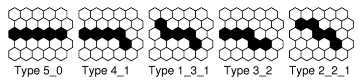
\includegraphics[width=0.8\textwidth]{./imgs/FD_straight_tracks.png}
	\caption{Fundamental shape of tracks considered straight. Image from \cite{FDReconstruction}.}
	\label{fig:fd-straight-tracks}
\end{figure}

\subsubsection{T3 trigger}
\label{sssec:t3-trigger}

T3 type triggers, or event type triggers are (with the exception of FD events, which have been discussed above) built from distributions of at least three SD 
stations next to each other that recorded a T2 trigger in close temporal succession. Upon the detection of such a pattern a readout command is issued to all nearby 
stations. Their recorded FADC traces as well as calibration information are forwared to CDAS if the station observed a T1/T2 event within an appropriate timespan 
of order $\mathcal{O}(\SI{}{\micro\second})$ before or after the T3 pattern occurence. Such a modus operandi enables an accurate reconstruction of the shower 
footprint by including stations that did not participate in the initial T3 trigger. This extends to FD issued T3 triggers, where potential information from SD 
stations in the vicinity of the FD-reconstructed shower core position is requested.

\subsection{Core position}
\label{ssec:core-position}

All reconstruction algorithms presented in the following subsections rely in one form or the other on an accurate determination of where the shower was recorded 
above the observatory. Hence the center of the shower footprint, the shower core, must be estimated at the beginning of the analysis chain. 

Without any prior knowledge, a first guess as to where the shower core is located can be made by calculating the barycenter of all participating stations. In this 
fashion, a weighted mean of all station locations is constructed with weights equal to the square root of the corresponding signal strength \cite{SDReconstruction}.

The presented approach fails if only parts of the shower are contained within the SD event. This occurs espically at the edges of the SD array, or in the vicinity
of faulty WCDs. A fiducial trigger, $N$T5, is employed to mitigate this problem. $N$T5 requires at least $N$ active stations around the SD detector that recorded 
the largest signal \cite{abraham2010trigger}.

\subsection{Arrival direction}
\label{ssec:arrival-direction}

The shower footprint measured by the SD (example given in \autoref{fig:shower-footprint}) corresponds to the projection of the shower plane onto the detector 
plane, i.e. the ground. It can be assumed that the shower plane has a fixed (hyperbolic \cite{bonifazi2005angular}) shape and propagates at the speed of light 
along the primary particles trajectory. With this knowledge, estimating the arrival direction becomes a task of minimizing the difference between measured and
expected arrival times given by an example shower axis anchored at the reconstructed shower core. The axis for which the summed differences is minimal corresponds
to the most likely arrival direction of the primary particle.

Naturally, the expected variance on the reconstructed $\phi$ and $\theta$ diminishes the more stations participate in the combined fit. The angular resolution thus
decreases for larger energies of the primary particle. This can be seen in \autoref{fig:angular-resolution}. In any case, the angular resolution even at smaller 
energies is better than $2.2^\circ$. For hybrid events, where the shower has also been detected by the FD, the angular resolution is greatly increased to about 
$0.6^\circ$ \cite{bonifazi2005angular}.

\begin{figure}
	\begin{subfigure}[b]{0.5\textwidth}
		\centering
		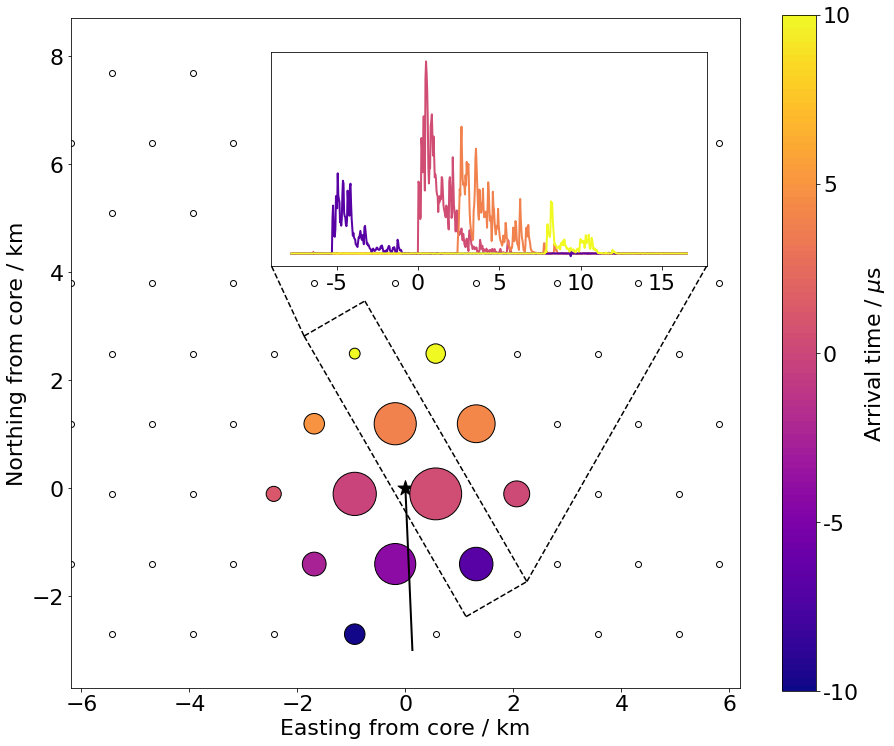
\includegraphics[width=\textwidth]{./plots/shower_footprint.png}
		\caption{\textbf{SD shower footprint}}
		\label{fig:shower-footprint}
	\end{subfigure}
	\hfill
	\begin{subfigure}[b]{0.5\textwidth}
		\centering
		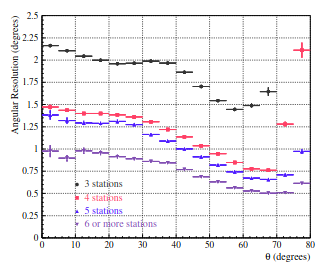
\includegraphics[width=\textwidth]{./plots/angular_resolution.png}
		\caption{\textbf{Angular resolution}}
		\label{fig:angular-resolution}
	\end{subfigure}
	\caption{
	\textbf{(a)} An example shower footprint recorded by the individual SD tanks (circles). The measured signal strength and arrival time is encoded in the	size 
	and color for each station. Tanks that haven't recorded any signal are shown colorless. For a subset of stations the respective VEM trace and consequently the
	propagation of the signal in the SD detector is shown in the inset plot on the top right.
	\textbf{(b)} The angular resolution as a function of $\theta$ for energies exceeding \SI{3}{\exa\electronvolt}. Image from \cite{bonifazi2005angular}.}
	\label{fig:offline-calibration}
\end{figure}

\subsection{Energy estimation}
\label{ssec:energy-estimation}

After a shower core has been pinpointed and the shower axis was determined, all information to fit an LDF is present. The \textbf{S}hower\textbf{P}lane 
\textbf{D}istance (SPD), the minimal separation between shower axis and station position, is calculated for each tank participating in the event and related to the
integrated signal $S$ (in units of \Qpeak) it received. From the so gathered lateral distribution of a shower the integrated signal $S_{1000}$ of a hypothetical 
(labelled dense) station laying at $\text{SPD} = \SI{1000}{\meter}$ is obtained.
This standardizes the comparison of results across many different events, even if a shower has only triggered few stations \cite{gaisser1977reliability}.

Due to attenuation effects in the atmosphere $S_{1000}$ is a function of $\theta$. It has been shown in \cite{DarkoCIC} that by separating the $\theta$ dependence
of a signal $S(\theta) = S\cdot A(\theta)$ and normalizing to a reference shower inclination, a reasonably unbiased estimator $S_{38}$ can be recovered via a 
\text{C}onstant \text{I}ntensity \text{C}ut (CIC) as shown in \autoref{eq:constant-intensity-cut-1} and \autoref{eq:constant-intensity-cut-2}.

\begin{equation}
\label{eq:constant-intensity-cut-1}
f_\text{CIC} = \frac{S_{1000}(\theta)}{S_{1000}(\theta_\text{ref})}=\frac{A(\theta)}{A(\theta_\text{ref})}.
\end{equation}

The reference angle is chosen as $\theta_\text{ref} = 38^\circ$, as this is the median inclination of detected events \cite{aab2020measurement}. It follows

\begin{equation}
\label{eq:constant-intensity-cut-2}
S_{38} = \frac{S_{1000}(\theta)}{f_\text{CIC}(\theta)}.
\end{equation}

Further corrections are applied to $S_{38}$ in order to counteract influence of the local weather or geomagnetic effects \cite{aab2020measurement}. What remains is a shower 
parameter which has been sanitized as much as possible from any environmental factors, and which has a proportionality to the energy of the primary particle, 
as discussed in \autoref{chap:extensive-air-showers}.

The approximate relation of $S_{38}(E)$ can be inferred from hybrid measurements, where the calorimetric energy as measured by the FD is connected to $S_{38}$.
From such datasets it follows the relation below, with the fit parameters for $A, B$ as determined in \cite{PhysRevD.102.062005}.

\begin{align*}
	\label{eq:SD-energy}
	E_\text{SD} = A \, (S_{38} /\; \SI{}{\Charge})^B \numberthis
\end{align*}

\vspace{-2em}

\begin{align*}
	A &= \SI{1.86\pm0.03e17}{\electronvolt} \\
	B &= 1.031\pm0.004 \\
\end{align*}

\subsection{Primary particle}
\label{ssec:primary-particle}

The determination of the primary particle, also referred to as the mass composition, relies on the systematic differences in air showers discussed in 
\autoref{sec:superposition-principle}. Muons, due to their noninteracting nature at high energies are typically the first signal to arrive in a WCD from an air
shower. Since high-mass primaries produce a higher fraction of muons this implies that the rise time, in which the integrated signal goes from $10\%$ to $50\%$ of
the total received signal, is shorter in these showers. Consequent analysis over a statistically relevant dataset thus reveals the mass composition of the cosmic
ray flux (compare \cite{letessier2014highlights}, \autoref{fig:cr-energy-spectrum})
	% %! TEX root = ../thesis.tex

\chapter{Neural networks}
\label{chap:neural-networks}

The idea of a \textbf{N}eural \textbf{N}etwork (NN) is to attempt to capture the human thinking process in machine code. For this purpose, a network architecture
connects some input (e.g. a picture) to an output (e.g. digits 0-9). Much like in a human brain, the architecture consists of multiple smaller chunks, neurons 
and layers, which connect in some way to form an emergent intelligence. 

As described, neural network do not yet hold the abilities to achieve their designated tasks, and can hardly be called intelligent. They need to be trained. 
This is done by presenting an example input (called training data) to the network. The network output is compared to the desired output for the given input via 
some loss function. During training, the network attempts to minimize this loss function. How it is minimized is often a design choice, and in general will 
depend on the network architecture, which in turn is influenced by the type of data and kind of task the NN should accomplish.

In the following several network architectures which are relevant for this work are detailed. The most simple option of a \textbf{D}ense NN (DNN) is given in 
\autoref{sec:DNN} in order to introduce several key concepts. \textbf{C}onvolutional NNs (CNNs) used for image recognition are explained in \autoref{sec:CNN}. 
Lastly \textbf{R}ecurrent NNs (RNNs) that find an application in time series analysis are shown in \autoref{sec:RNN}

\section{Dense neural network}
\label{sec:DNN}

Dense neural networks are subdivided into layers, which themselve consist of individual neurons.


\section{Convolutional neural network}
\label{sec:CNN}

\section{Recurrent neural network}
\label{sec:RNN}
	% % !TEX root = ../thesis.tex

\chapter{Neural network training data}
\label{chap:neural-network-data}

Over their relatively brief existance, neural networks have been shown to perform increasingly impressive tasks (e.g.  \cite{openai2019dota}, \cite{openai2023gpt4}, 
and many more). However, they learn by example. The performance of a neural network is directly linked to the input data it receives during training. If the 
training data is not an accurate example of real world information a network later operates on, insight gained from it is at best an approximation, and at worst
completely randomly generated data. 

As such, it is not a question \textit{if} some neural network architecture can learn to identify an extensive air shower from WCD data, but rather which 
implementation, fed with which information, does. For this purpose, this chapter explains the procedure with which training data is generated. As stated above, this
must occur with a focus on being representative of data actually measured in the SD array. The elected approach to create time traces is modularized. The structure
of this chapter reflects this. First, general comments about the characteristics of background data (i.e. the WCD detector response in the absence of an extensive 
air shower) are made in \autoref{sec:background-dataset}. Next, the process to extract signal originating from CRs is detailed in \autoref{sec:signal-dataset}.
Lastly, building the time trace from the aforementioned modules and drawing samples from it for a neural network to train on is done in \autoref{sec:trace-building}.

\section{Background dataset}
\label{sec:background-dataset}

While a flux of partices causes elevated ADC levels in both the HG and LG channels of a WCD PMT during a shower event, the lack of such a phenomenon does not imply 
the readout information is uniformly flat. Instead, it hovers around the channels' baseline (c.f. \autoref{sec:surface-detector}) with occasional spikes upwards 
due to low-energy particles impinging on the detector. Coupled with electronic noise from the many digital components in the station electronics, the 
\textbf{U}pgraded \textbf{U}nified \textbf{B}oard (UUB), this constitutes the data that is collected inbetween air shower events.

\subsection{Accidental muons}
\label{ssec:accidental-muons}

Most low-energy background particles present in the detector are muons. These are produced in the upper atmosphere during cascading processes analog to 
\autoref{chap:physical-background}. Due to the low primary energy the electromagnetic component of the shower is thermalized before it reaches surface level. The 
muonic component by itself does not contain enough information to enable an accurate reconstruction of primary energy and origin. This fact, coupled with the high
flux of events at lower energies ($\Upphi|_{E=\SI{100}{\giga\electronvolt}} \approx \SI[per-mode=power]{1}{\per\meter\per\second}$ \cite{boezio2000measurement}) 
make these events unsuitable for analysis. Stray muons, even though they originate from extensive air showers, must consequently be considered background events.

The rate at which such particles traverse a WCD tank is $f_\text{Acc.}\approx\SI{4.665}{\kilo\hertz}$ \cite{DavidBackgroundSim}. Their arrival time is 
Poisson-distributed. This implies that generally, one in 14 time traces contains signal from a low-energy background event. Coincidences of two accidental 
muons occur on a sub-percent level. Any higher order of coincidences is likely originating from a single air shower process. The typical signal recorded by the 
surface detector from a single muon is presented in \autoref{fig:muon-response}.

\begin{figure}
	\centering
	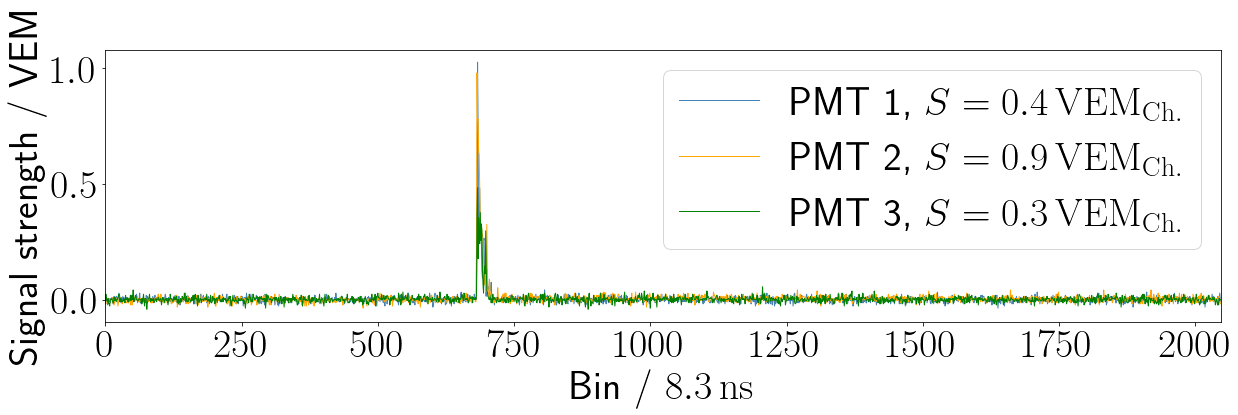
\includegraphics[width=0.8\textwidth]{./plots/muon_response.png}
	\caption{The simulated time trace from a single muon. The maximum peak of the time trace is equal to \SI{1}{\Peak}. The integral over each PMT, $S$, sums to
    $\approx\SI{1}{\Charge}$.}
	\label{fig:muon-response}
\end{figure}

A library of background traces of this type was provided by David Schmidt \cite{DavidBackgroundSim}. However, only the largest response of the three WCD PMTs is
available for this library. Due to the lack of information one is either forced to assume the response to a low-energy background particle is the same across all 
PMTs, or neglect the response of the two remaining PMTs altogether upon injectiong a background muon into a signal trace (c.f. \autoref{sec:trace-building}). In 
both cases, neural networks are provided an easily detectable pattern to discern such particles from "real" shower signal. As a result, it should be refrained 
from training AI triggers on this dataset.

\subsection{Electronic noise}
\label{ssec:electronic-noise}

Electronic noise is the umbrella term given to the distortions that some signal is subject to during digital readout. Such noise can have many different origins.
An illustrative example is given by the \textbf{L}aser \textbf{I}nterferometer \textbf{G}ravitational wave \textbf{O}bservatory, which excludes the \SI{60}{\hertz}
band and its' harmonics from analysis. This is owed to the fact that the DC frequency standard in the United States introduces systematic uncertainties in the
detector \cite{martynov2016sensitivity}. In the electronics of Pierre Augers' SD array, electronic noise is assumed to be Gaussian. That is to say that the 
\SI{}{\ADC} values of a time trace that was measured while no particle produced signal in the tank are normally distributed around the baseline. The standard 
deviation can be estimated from monitoring data, as is shown in \autoref{fig:random-traces}.

\subsection{Random traces}
\label{ssec:random-traces}

Both above mentioned phenomena can be simulated, and the simulation results used as background training data for the neural networks discussed in the next chapter.
A more accurate method however, and the approach elected for this work is to utilize directly measured data from the field. Thanks to the work of David Nitz, there 
exist collections of so called random-traces\footnote{to avoid possible confusion between this dataset and a \textit{random} trace in the statistical sense, the 
traces recorded by David Nitz are referred to as random-trace, with a hypen.} that were gathered by forcing DAQ readout via a manually set trigger. 

In particular, two datasets of UUB random-traces have been created until now. They were taken from 13th-18th March 2022, and 14th-18th November 2022 respectively. 
The first set contains data a total of sixteen million time traces distributed over four different SD stations. For reasons explained in 
\autoref{ssec:random-trace-calibration}, only data from the first set is used in the analysis presented in this work.

\subsubsection{Characteristics}
\label{ssec:random-trace-characteristics}

Contrary to the naming of the random trigger, it occurs at a deterministic time. More accurately, the process of measuring random-traces is as follows;
A single time trace ($2048\cdot\SI{8.333}{\nano\second} = \SI{17.07}{\micro\second}$) is written to the local station buffer every $\SI{10}{\milli\second}$. Once
the buffer has accumulated enough data, it is written to a USB storage device. Because of a bottleneck in the last step, the process takes about \SI{22}{\hour}
per station \cite{nitzCorrespondence}.

It is thus not the trigger that is unpredictable, but the data measured by each trigger. Due to the read/write process being indepentant of the measured data
(as opposed to the algorithms in \autoref{chap:classical-triggers}) the latter must be considered to be essentially random. For the most part, random-traces are 
assumed to consist solely of electronic noise. However, signal of cosmic origin - be it accidental muons or extensive air showers - will appear in the data at a
rate at least consistent with \autoref{sec:classical-triggers-performance}.

A crude analysis of the type of noise in the random-traces can be made by examining the spectral density of the dataset, shown in \autoref{fig:random-traces}.
Harmonic modulations visible in both spectra might originate from an offset between last and first bin of the random-traces. If this offset is nonzero, the 
periodic extension of $f(x)$ exerts a step-function-like behaviour. The Fourier transform consequently reflects this \cite{burrows1990fourier}. Still, several
features of $| \hat{f}(\xi) | ^{2}$, espically present at $\SI{10}{\mega\hertz}$, imply the presence of systematic noise in the UUB. Nevertheless, the large scale 
form of the spectral density is compatible with at least two noise models, that cannot be distinguished based on the data at hand:

\begin{itemize}
	\item  $\mathbf{| \hat{f}(\xi) | ^{2} \propto \exp\left(\frac{(\xi - \mu)^2}{2\sigma^2}\right)}$. The spectral density is Gaussian. This implies the noise is 
	Gaussian distributed as well, confirming the assumption in \autoref{ssec:electronic-noise}.
	\item $\mathbf{| \hat{f}(\xi) | ^{2} \propto} \exp\left(-m\xi + b\right)$. The spectral density is proportional to $\xi^{-n}$ for some power $n$. The case 
    $n = 2$ ($\SI[per-mode=symbol]{-6}{\deci\bel\per\octave}$ attenuation) seems to describe the observations well, hinting that the generating function could be 
    Brownian.

\end{itemize}

\begin{figure}
	\centering
	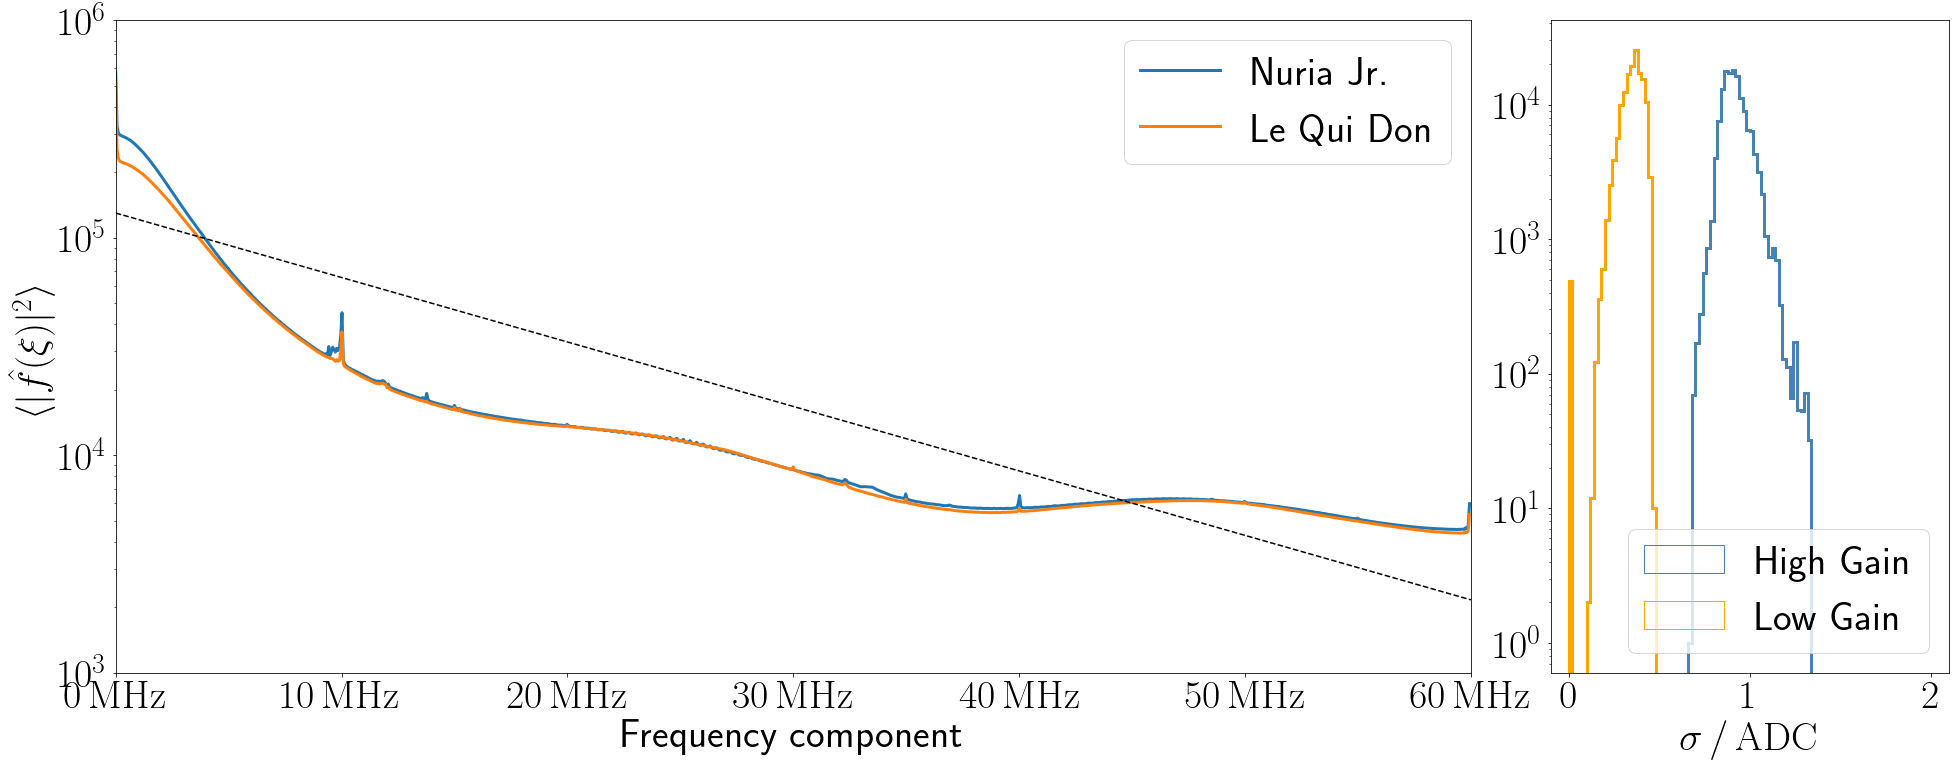
\includegraphics[width=0.8\textwidth]{./plots/fft_variance_plot_combined.png}
	\caption{(\textit{Left}) The random-trace spectral density for two stations. Plotted with a dashed black line is reference attenuation curve falling at 
	$\SI[per-mode=symbol]{-6}{\deci\bel\per\octave}$. The spike at \SI{10}{\mega\hertz} is of unknown origin and represents systematic noise in the UUB 
	electronics. (\textit{Right}) Example variance of all UUB stations in the surface detector array. The data shown in this plot was recorded on November 15th 
    2022.}
	\label{fig:random-traces}
\end{figure}

\subsubsection{Calibration}
\label{ssec:random-trace-calibration}

The random-trace files contain raw measurement data in units of $\SI{}{\ADC}$ for the HG and LG channel of the three WCD PMTs. In a first step to standardize this
information, the baseline is substracted from each FADC bin. This is done via the baseline finding algorithm described in \autoref{ssec:offline-calibration} and 
\cite{tobiasBaseline, tobiasBaselineUUB}. Note that this approach differs from the baseline finding algorithm that runs on each station (c.f. 
\autoref{ssec:online-calibration}). However, the difference is negligible ($<<\,\SI{1}{\ADC}$) for traces that do not contain any signal, which is the case for the 
vast majority of the dataset.

Next, the baseline-substracted time traces are converted from units of $\SI{}{\ADC}$ to $\SI{}{\Peak}$. This conversion is not straight forward, as it requires 
knowledge of \Ipeak at the time of data taking. Each station estimates this value in periodic time intervals in the context of monitoring diagnostics.

For the second dataset of random-traces (taken from 14th-18th November 2022) a UNIX timestamp packaged with each time trace may be related to monitoring data. This 
reveals that no information regarding \Ipeak was forwarded to CDAS for any station while it recorded random-traces. As a result, the entire dataset is unfortunately 
rendered useless for this work.

For the first collection of random-traces, monitoring data is available, but there exists no timing information for the individual traces. Only the date of the 
measurement is known. The elected procedure to evaluate data as accurately as possible is thus to calculate the day average of \Ipeak and \Qpeak and take this as 
the best (first) estimate for each trace. As can be seen in \autoref{fig:random-trace-diagnostics}, this eliminates half of the remaining dataset, as two of the four 
stations show a large variance in \Ipeak. The day average in these particular cases is not a good estimator for calibration purposes. For this reason, only random 
traces from the stations Nuria and Le Qui Don, measured in the March dataset are used for analysis purposes, as their $I_\text{VEM, Rand.}$ is stable.

As a crosscheck to verify the goodness of the approximation, the T2 trigger rate as reported by the calibration process is related to the trigger rate obtained by
direct calculation over all (calibrated) random-traces. By extension, this also serves as a unit test for the classical triggers as they will be implemented in 
\autoref{chap:classical-triggers}. The results of this analysis are shown in \autoref{fig:random-traces-correction}. As is clear from the plot, the rates 
calculated from the two different approaches are not in accordance. This indicates systematic errors in the calibration (a wrong implementation of trigger 
algorithms is disfavoured from the discussion in \autoref{chap:classical-triggers}). The errors are consistent across both considered stations. It is found that 
calculated trigger frequencies are $\approx25\%$ lower than what is taken from monitoring. It is unclear why this discrepancy occurs, as it implies that the 
stations do not use the same threshold values for triggering as they report.

In any case, $I_\text{VEM, Rand.}$ must be adjusted to reflect this. A $25\%$ increase in trigger rate is relatable to a $\approx10\%$ decrease in \Ipeak. The 
calibration scaling factors for random-traces thus become the values listed in \autoref{tab:I-peak-random}.

\begin{table}
	\begin{center}
	\caption{Calibration constant \Ipeak for random-traces.}
	\begin{tabular*}{0.6\textwidth}{@{\extracolsep{\fill}} c|c|c}
		\toprule
		PMT \# & Nuria & Le Qui Don \\
		\midrule
		1 & \SI{159.34}{\ADC} & \SI{145.79}{\ADC} \\
		2 & \SI{161.37}{\ADC} & \SI{144.63}{\ADC} \\
		3 & \SI{149.91}{\ADC} & \SI{154.62}{\ADC}
	\label{tab:I-peak-randoms}
	\end{tabular*}
	\end{center}
\end{table}

\begin{figure}
	\centering
	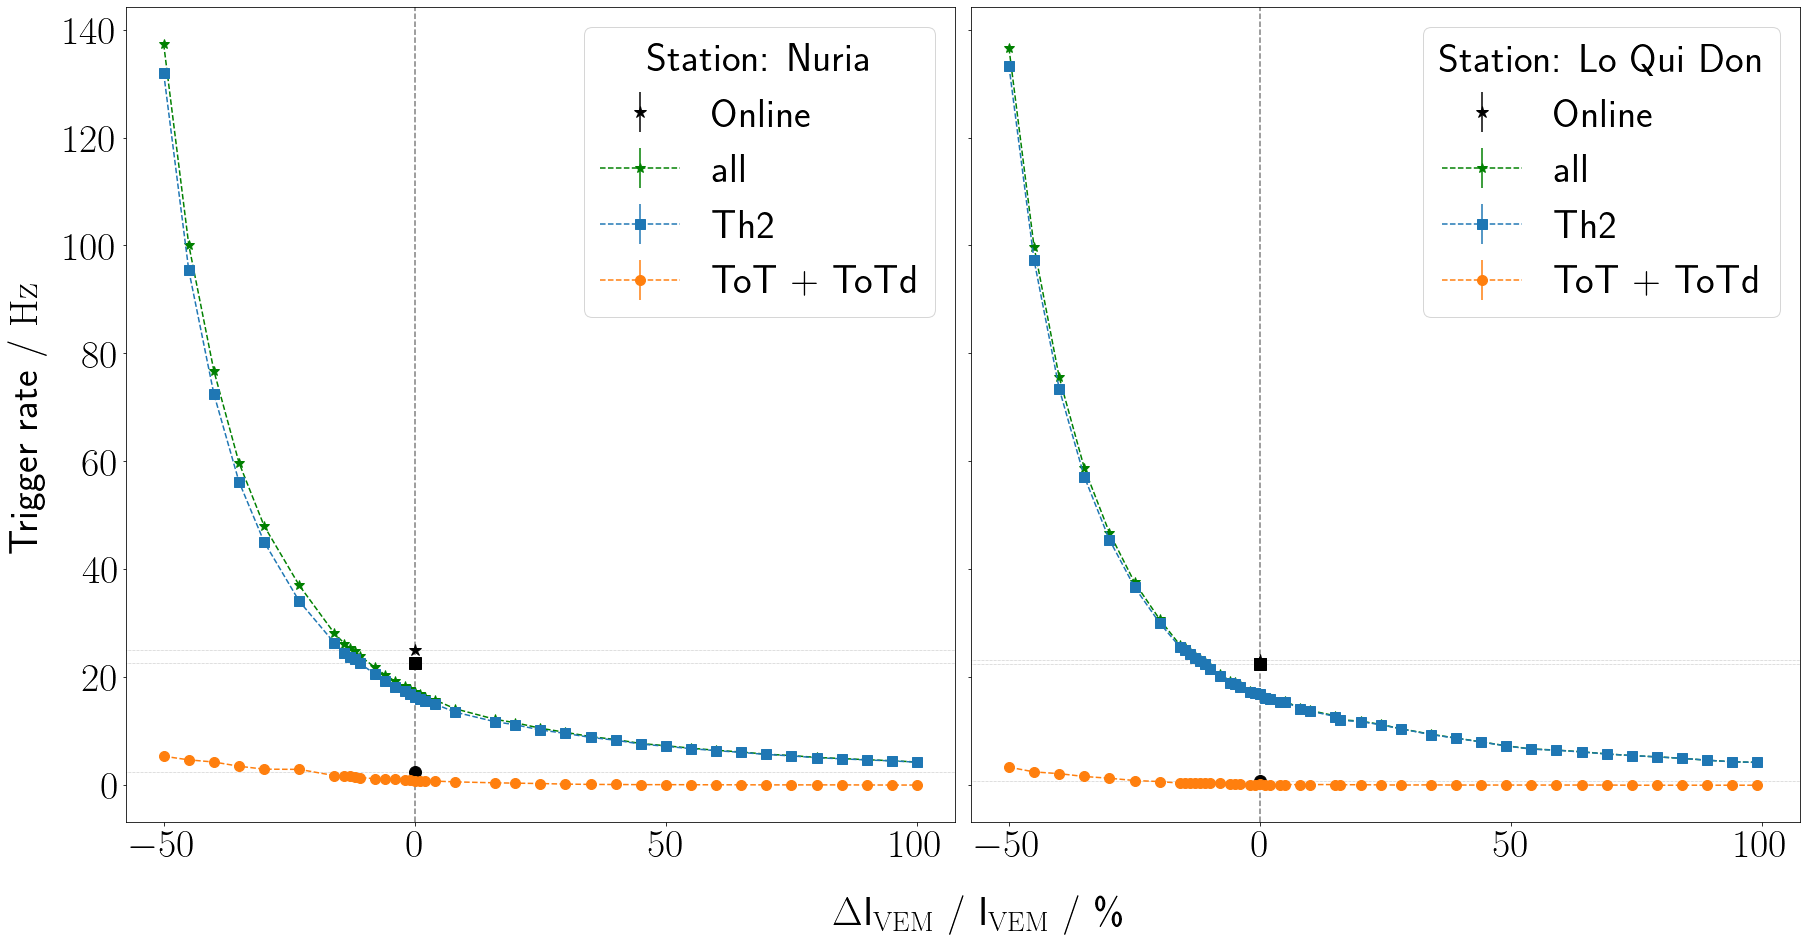
\includegraphics[width=\textwidth]{./plots/random_traces_correction_factor.png}
	\caption{The online reported T2 trigger rate (black) does not match the calculated trigger rate. Only a decrease $\Delta$\Ipeak by $1/10$th of the original 
	\Ipeak gives a close approximation of the observed rate when manually calculating trigger frequencies.}
	\label{fig:random-traces-correction}
\end{figure}

\begin{landscape}
    \begin{figure*}
        \centering
        \begin{subfigure}[b]{0.5\textwidth}
			\hspace{-4cm}
            \centering
            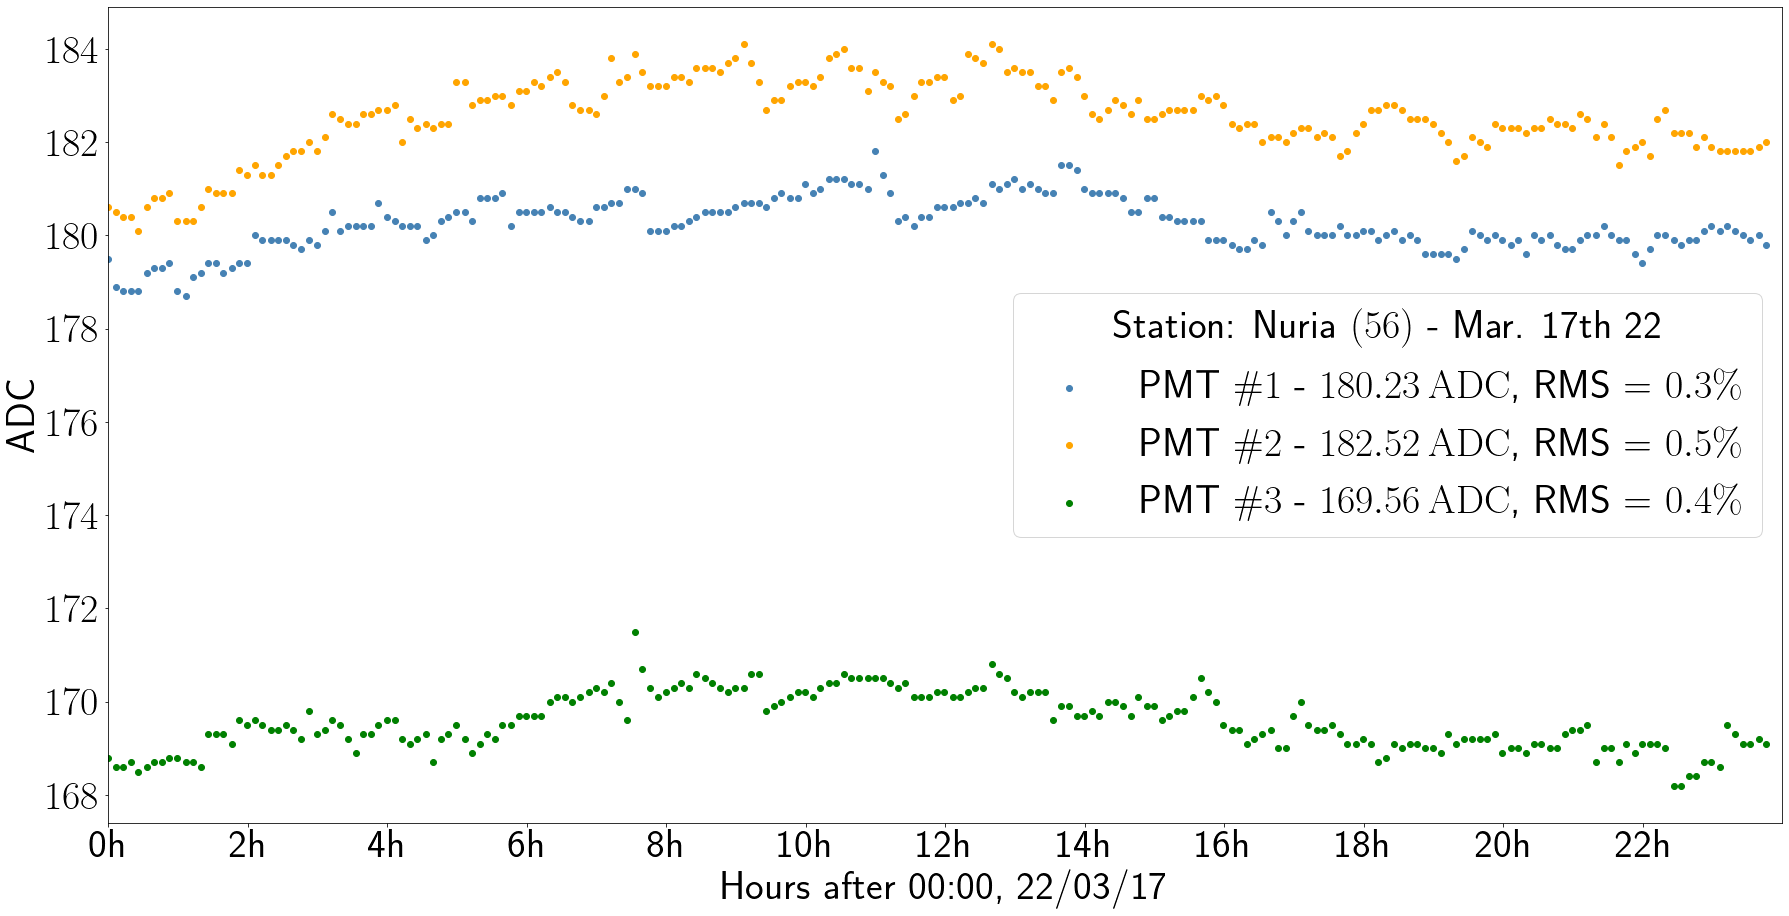
\includegraphics[width=0.7\textheight]{./plots/random_trace_diagnostics_nuria.png}
        \end{subfigure}
        % \hfill
        \begin{subfigure}[b]{0.5\textwidth}  
            \centering 
            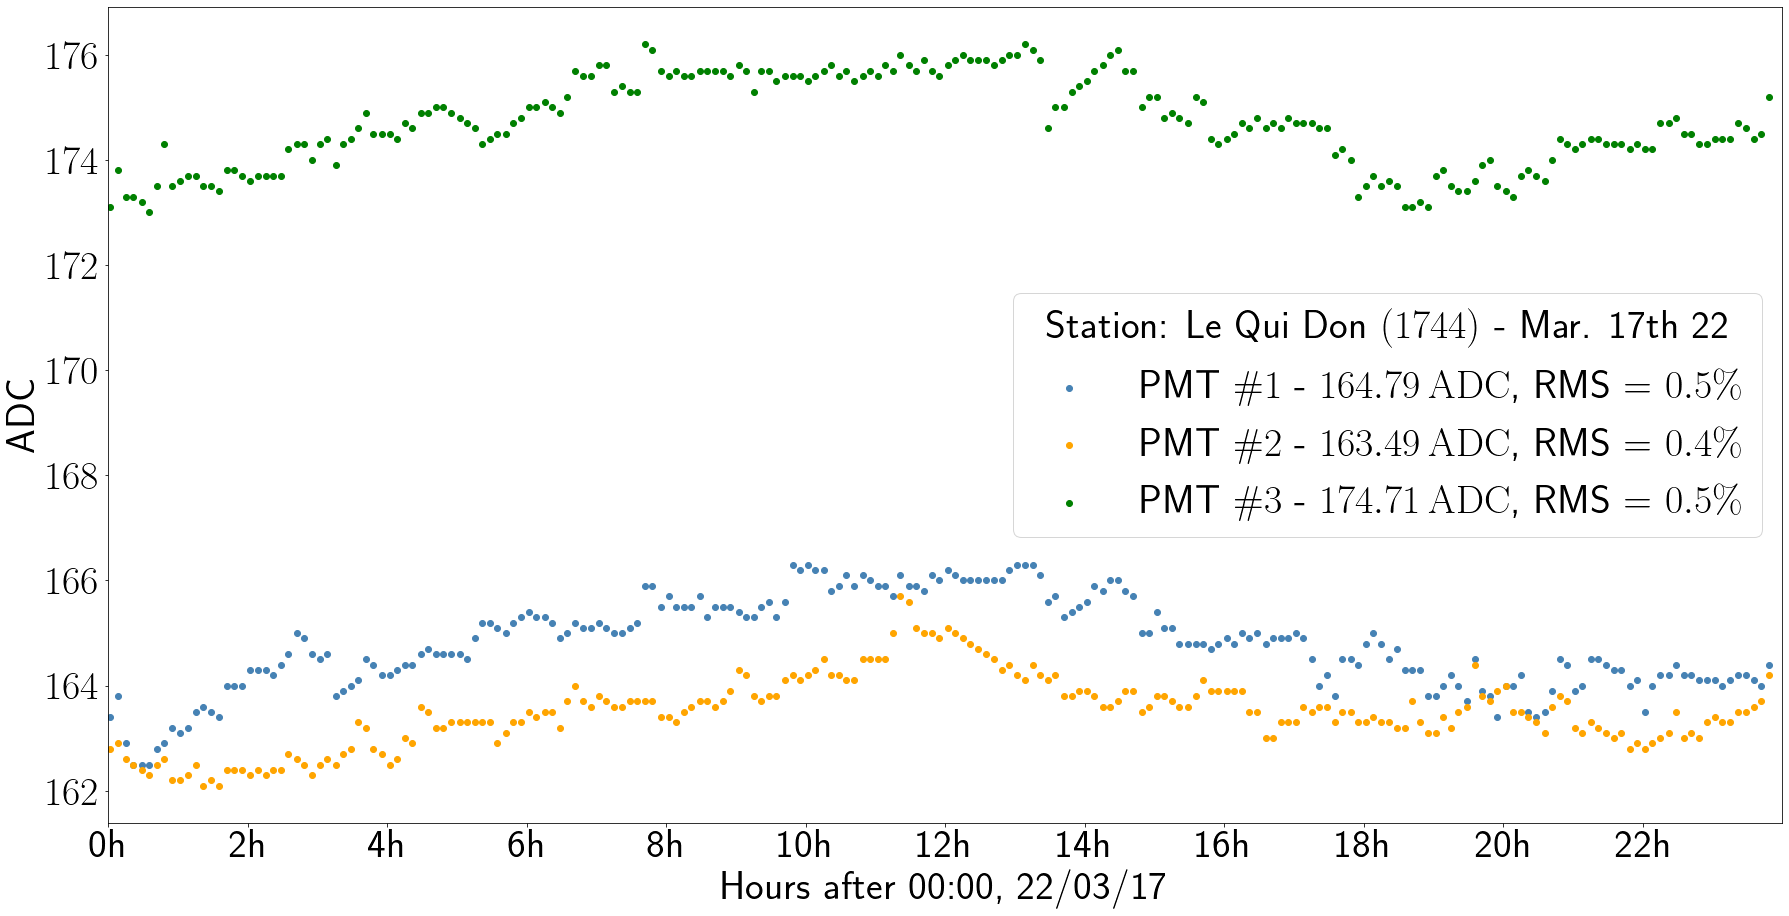
\includegraphics[width=0.7\textheight]{./plots/random_trace_diagnostics_le_qui_don.png}
        \end{subfigure}
        \vskip\baselineskip
        \begin{subfigure}[b]{0.5\textwidth}
			\hspace{-4cm} 
            \centering 
            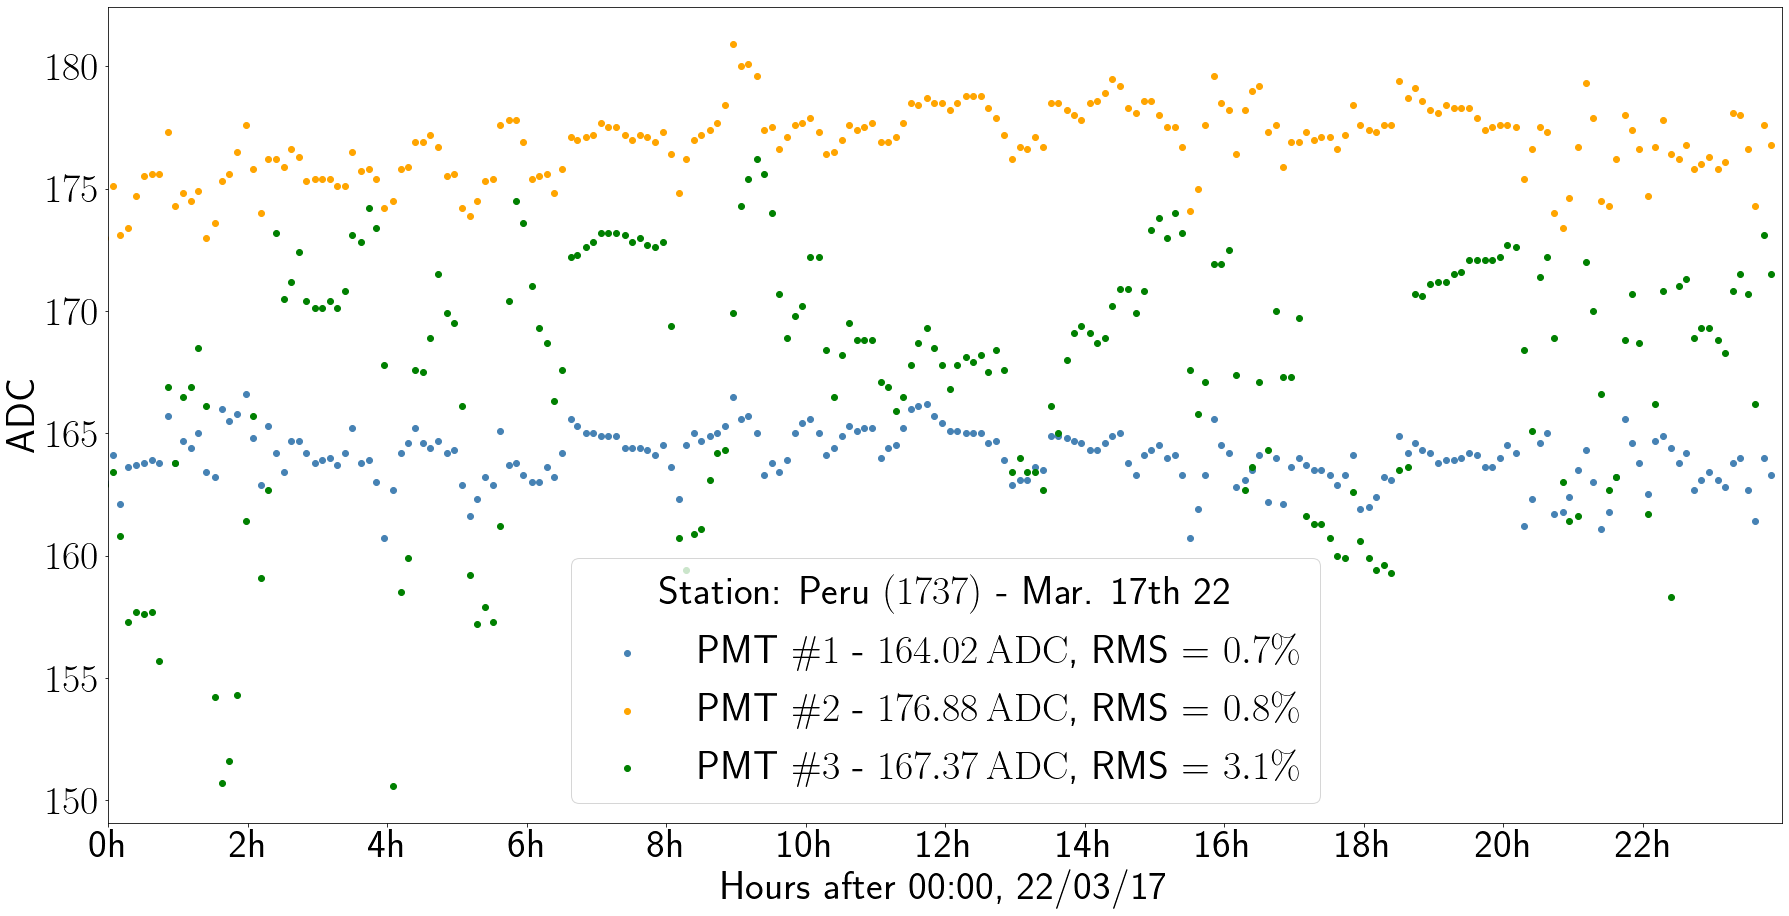
\includegraphics[width=0.7\textheight]{./plots/random_trace_diagnostics_peru.png}
        \end{subfigure}
        % \hfill
        \begin{subfigure}[b]{0.5\textwidth}   
            \centering 
            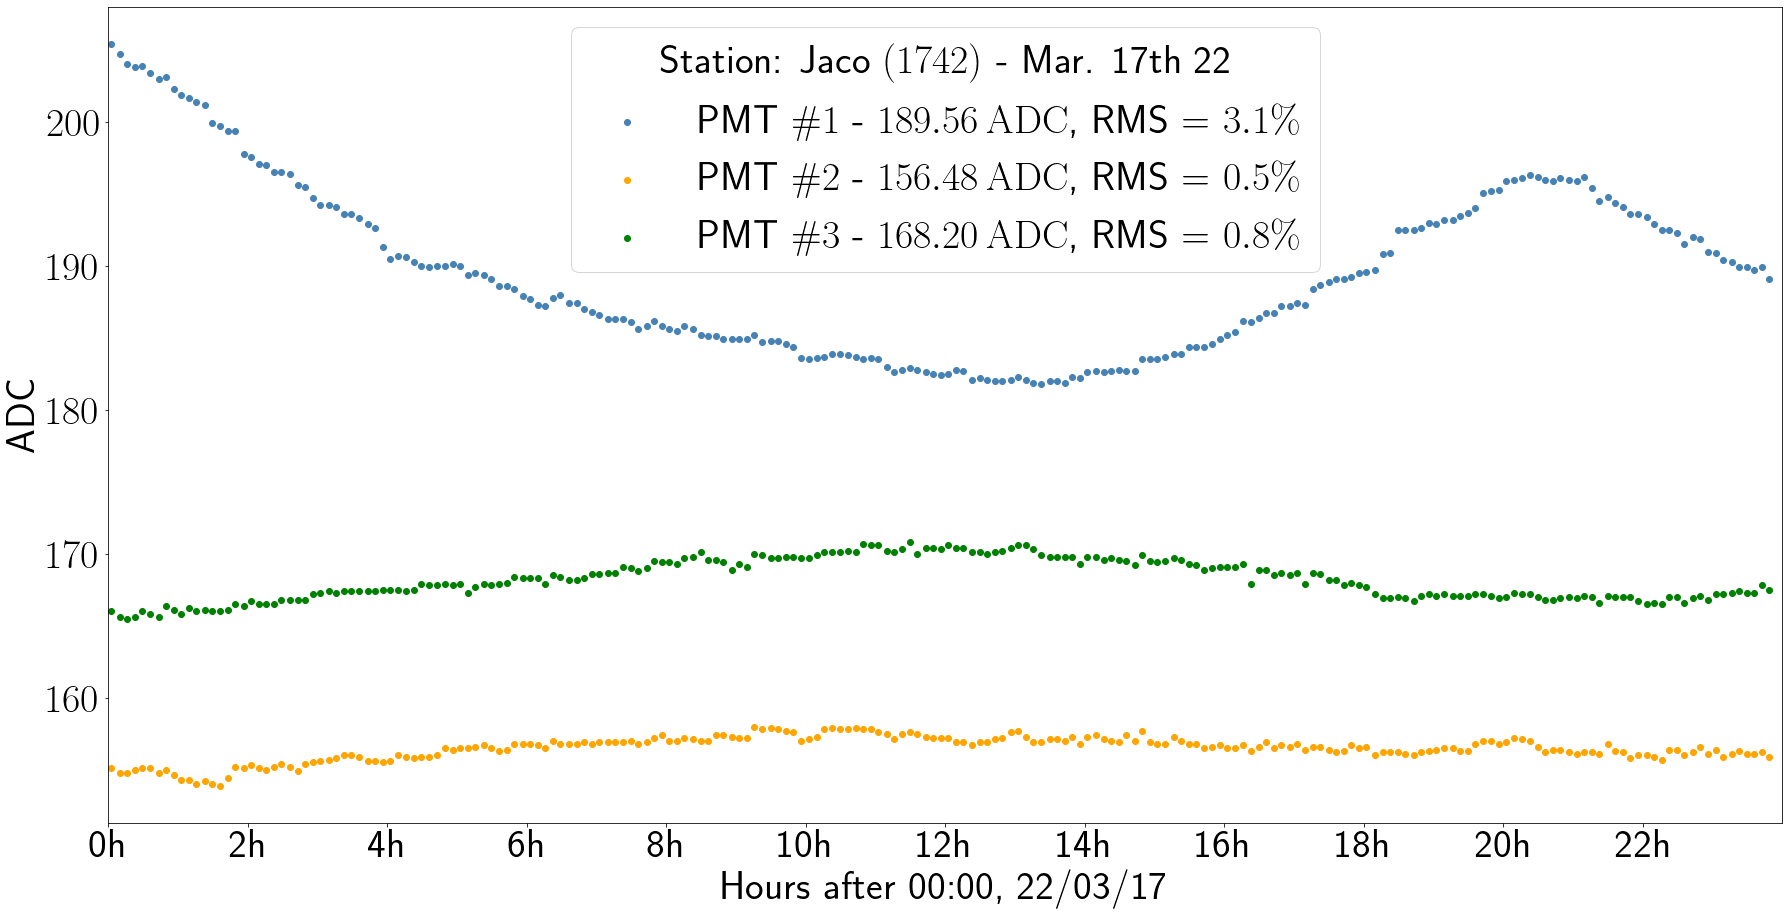
\includegraphics[width=0.7\textheight]{./plots/random_trace_diagnostics_jaco.png}
        \end{subfigure}
        \caption{Monitoring values for the four stations available in the random-trace dataset measured in March '22. The bottom two stations show a large variance
		in \Ipeak for at least one PMT. The two stations in the first row (Nuria, Le Qui Don) are more stable ($\sigma\,/\,\mu < 1\%$).} 
        \label{fig:random-trace-diagnostics}
    \end{figure*}
\end{landscape}

\section{Signal dataset}
\label{sec:signal-dataset}

In the context of this work, a "signal" (as opposed to background) is \textit{any} detector response caused by extensive air showers. Admittedly, this choice of 
classification is not ideal, as the particle density far from the shower axis grows sparse. Time traces recorded at those locations look very similar to ones 
raised by accidental muons. In any case, ramifications and possible solutions to this problem are further discussed in the following chapters. 

In order to isolate the signal stemming from shower particles only, an \Offline simulation using Geant4 is executed on CORSIKA source files \cite{heck1998corsika}.
These are a total of $40557$ simulated showers with a proton primary of energy $16 < \log\left(E/\SI{}{\electronvolt}\right) < 19.5$.  All showers are simulated 
using the hadronic interaction model QGSJET-II.04 \cite{ostapchenko2007status}.

In the process, the electronic feedback of the WCD PMTs is evaluated without any disturbance factor (see \autoref{sec:background-dataset}). That is to say that 
the time trace obtained from such simulations is identically zero (in units of \SI{}{\ADC}) at any point in time where no ionizing particles are present in the 
WCD. An example trace that visualizes this is shown in \autoref{fig:component_adding}. Next, the trigger conditions both for individual stations and on the 
event-level are altered to trigger on everything. This step is needed in order to save all traces to the simulation output, an \textbf{A}dvanced \textbf{D}ata 
\textbf{S}ummary \textbf{T}ree (ADST). If this was not the case, only traces that already satisfy current trigger conditions would be written to disk. A neural 
network training on such data could therefore at best be as efficient as the current triggers.

The choice of this approach forces some detours in the ADST readout. Instead of extracting the VEM calibrated traces directly, individual component traces, i.e. 
the PMT signal caused by muons, electrons and photons individually are summed to yield a total \SI{}{\ADC} trace. Signal stemming from hadrons or other components 
in the cascade is neglected. This does not impose any errors in the analysis, as the hadronic component espically lays close to the shower core, where the EM- and 
muonic component of the shower alone should already enable easy detection. Finally, the total trace as calculated above is extracted to a more easily accessible 
data format alongside shower metadata like primary energy, zenith, but also SPD, and particle count in the station the trace was recorded from.

\begin{figure}
	\centering
	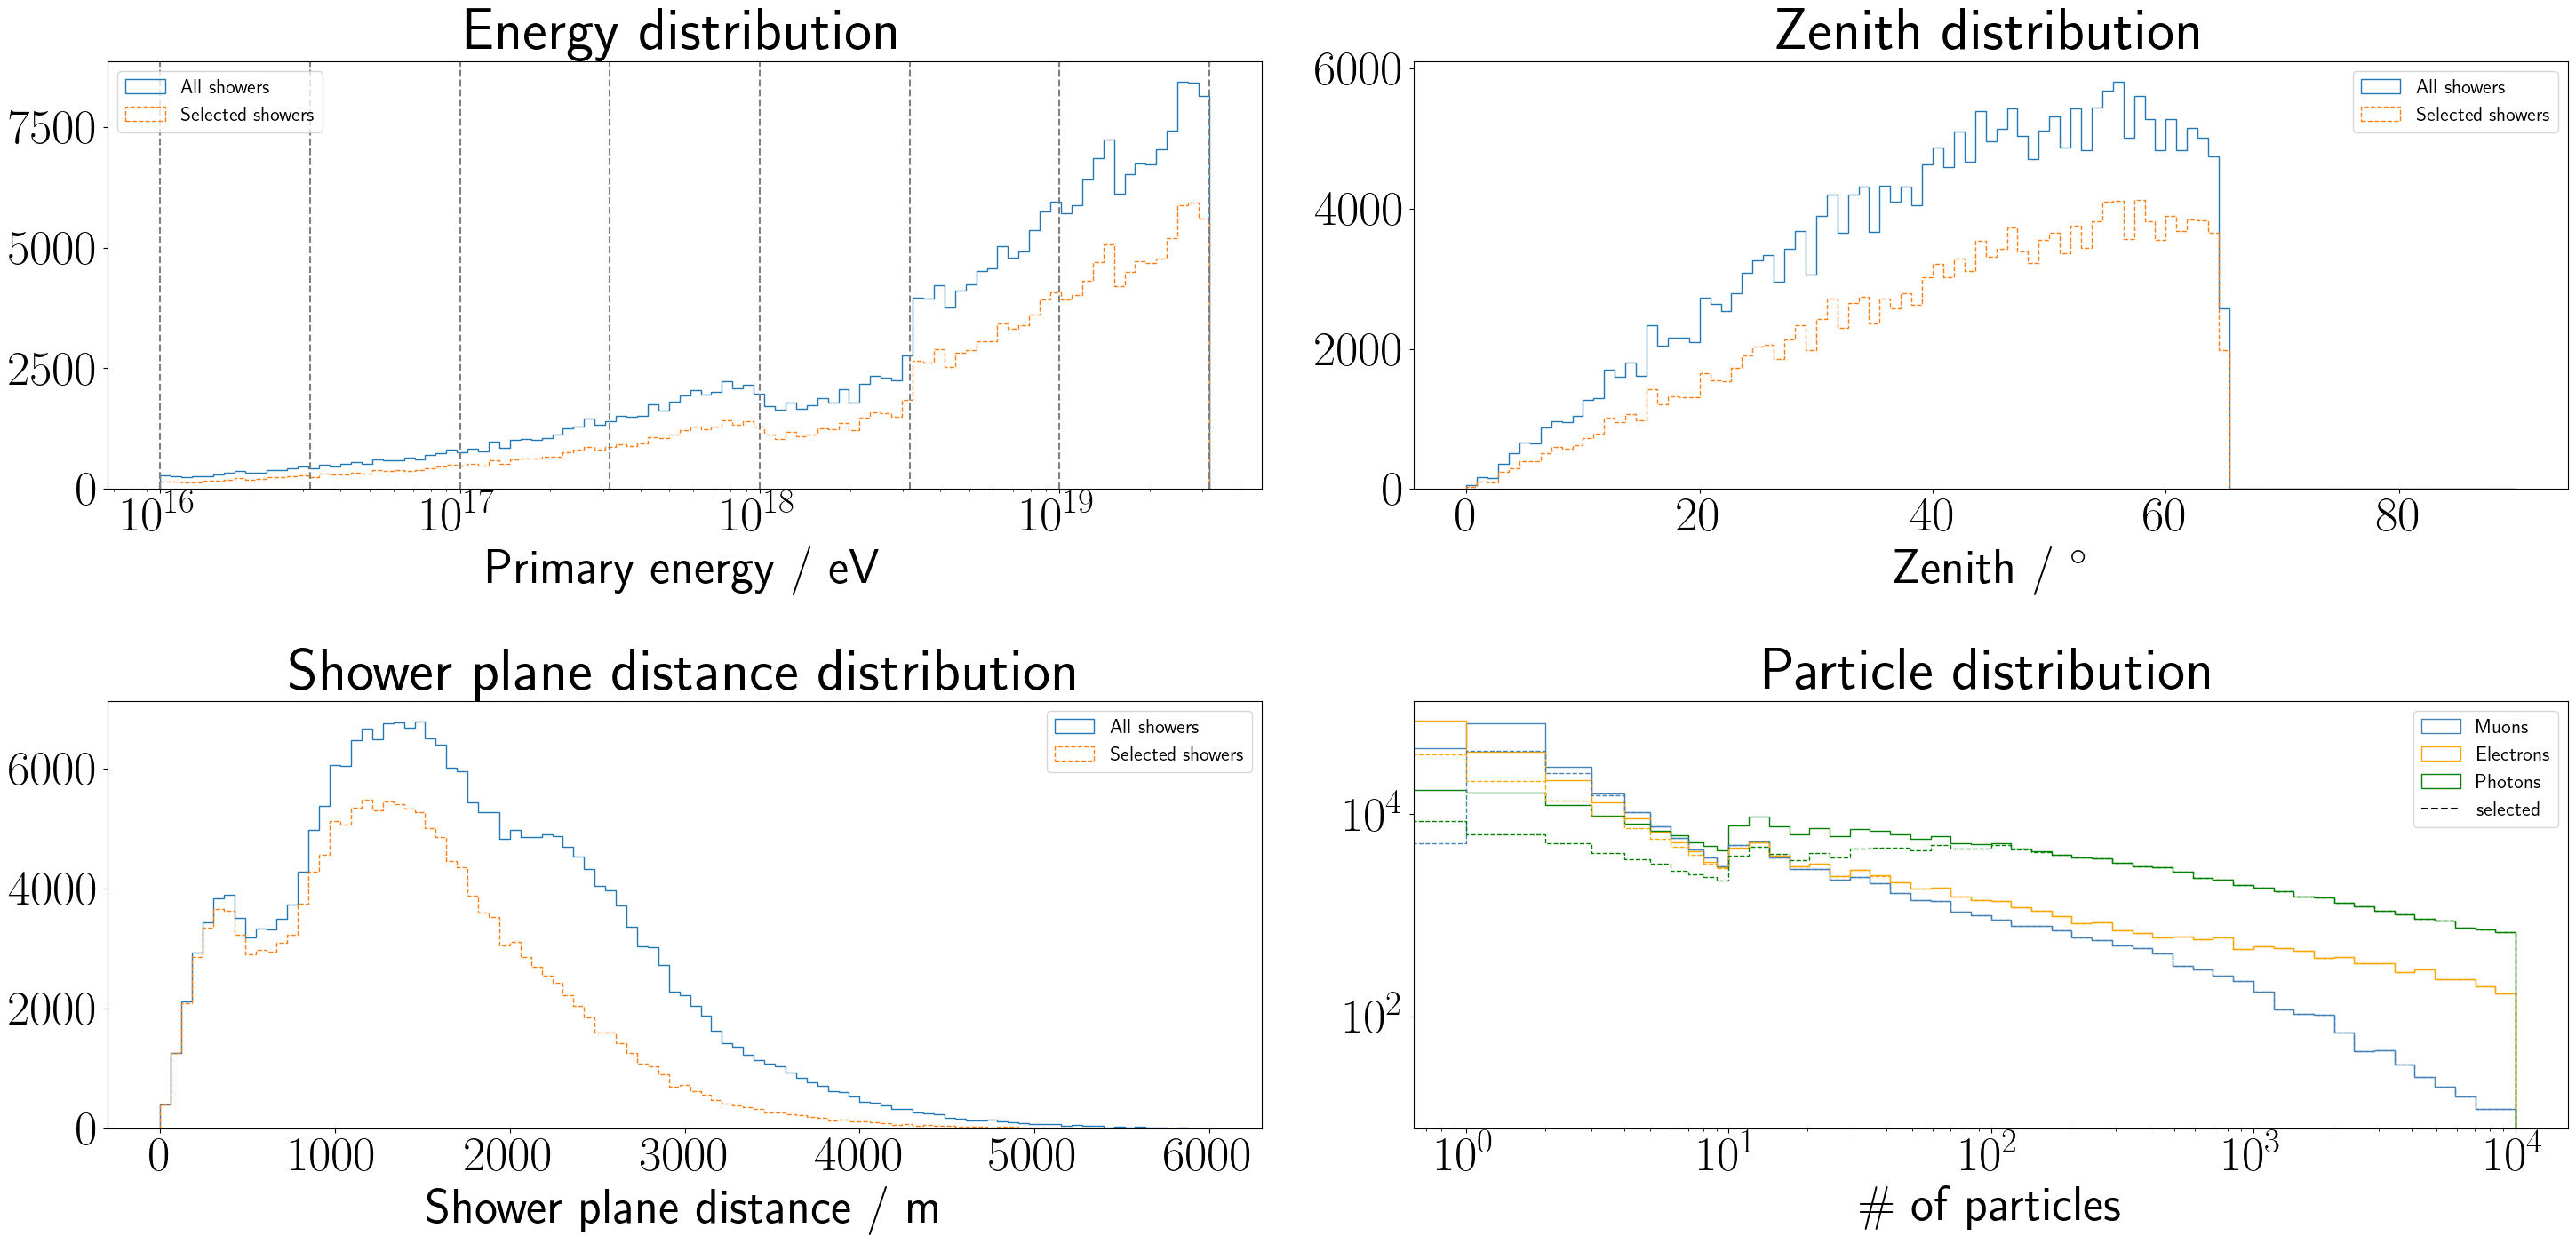
\includegraphics[width=1\textwidth]{./plots/physics_statistics.png}
	\caption{The distribution of primary energy (\textit{top left}), shower inclination (\textit{top right}), separation from shower axis (\textit{bottom left}), 
	and number of particles in a tank (\textit{bottom right}) is histogrammed for each trace available in the dataset. Since showers with higher primary energy 
	reach a larger number of stations, traces from showers with increasing energy are overrepresented in this dataset. The dashed lines in each subplot represent 
	the population of traces that deposit a signal 
	$S>\SI{}{\Charge}$ in the tank.}
	\label{fig:physics-data}
\end{figure}

\section{Trace building}
\label{sec:trace-building}

With the componentwise traces at hand, the total trace as would be recorded in the WCD PMTs for a given event, can be constructed. First, a trace container with 
default UUB trace length ($2048\,\text{bins}\cdot8.3\,\mathrm{ns}\,/\,\text{bin}=\SI{17.07}{\micro\second}$) and three components per bin (the three WCD PMTs) is 
initialized with all values equal to zero. Next, an arbitrary random-trace is selected as baseline. Since the FPGAs fundamentally count in the integer domain, the 
\SI{}{\ADC} data in the random-trace contains only whole numbers. As is, this wouldn't correctly model rollover when adding integer random-traces to floating point
simulation information. While two \SI{}{ADC} signals by themself might not exceed the threshold to cross to the next higher value, their sum would might; 
$\lfloor \SI{0.7}{\ADC} \rfloor + \lfloor \SI{0.4}{\ADC} \rfloor = \SI{0}{\ADC} \neq \SI{1}{\ADC} = \lfloor \SI{0.7}{\ADC} + \SI{0.4}{\ADC} \rfloor$. To account 
for this, uniformly distributed random numbers from 0 (inclusive) to 1 (exclusive) are added to the random-trace. 

Furthermore, the $I_\text{VEM, Rand.}$ from random-traces (c.f. \autoref{ssec:random-traces}) will in general be different from \Ipeak simulated by 
\Offline ($I_\text{VEM, Off.} = \SI{215.781}{\ADC}$ compare \cite{offlineSource}). Thus the random-trace must be scaled by a factor 
$\frac{I_\text{VEM, Off.}}{I_\text{VEM, Rand.}}$ before being added to the container. 

If desired, accidental muons can be added to the trace container as well. This is done either by directly specifying a number of random injections, or throwing the
dice according to the injection frequency specified in \autoref{ssec:accidental-muons}. If the number of accidental muons is nonzero, a sample of random background
traces from \cite{DavidBackgroundSim} is drawn and each sample added to every PMT at a random uniform position somewhere in the trace. 
\autoref{fig:component_adding} shows an example where five muons are injected into the trace.

Last, the actual shower signal is added to the trace container. In principle, it can be added at any random position, similar to the random injections. However, 
for continuity reasons and ease of comparing to plots generated with other software, the latch bin for signal insertion is hardcoded to be the same as in \Offline,
bin $660$. Since otherwise the data is in the correct $\SI{}{\ADC}$ format, no further manipulation of the data is necessary.

The trace container now holds all necessary components together, but remains in units of \SI{}{\ADC}. To convert to \SI{}{\Peak}, each bin in each PMT trace is 
floored to mimic the FPGA digital counting, and divided by the appropriate scaling factor \Ipeak times a correction factor that stems from a bias in the online 
peak estimation algorithm (see \cite{bertou2006calibration}). If traces need to be UB compatible the FADC bins must be filtered and downsampled in an intermediate 
step. This influences the scaling factor $I_\text{VEM, compat.}$ in a major way (compare \autoref{ssec:filtering-and-downsampling}). If the so-called 
full-bandwidth, UUB time trace is analyzed, the appropriate factor becomes $I_\text{VEM, Off.}$.

\begin{figure}
	\centering
	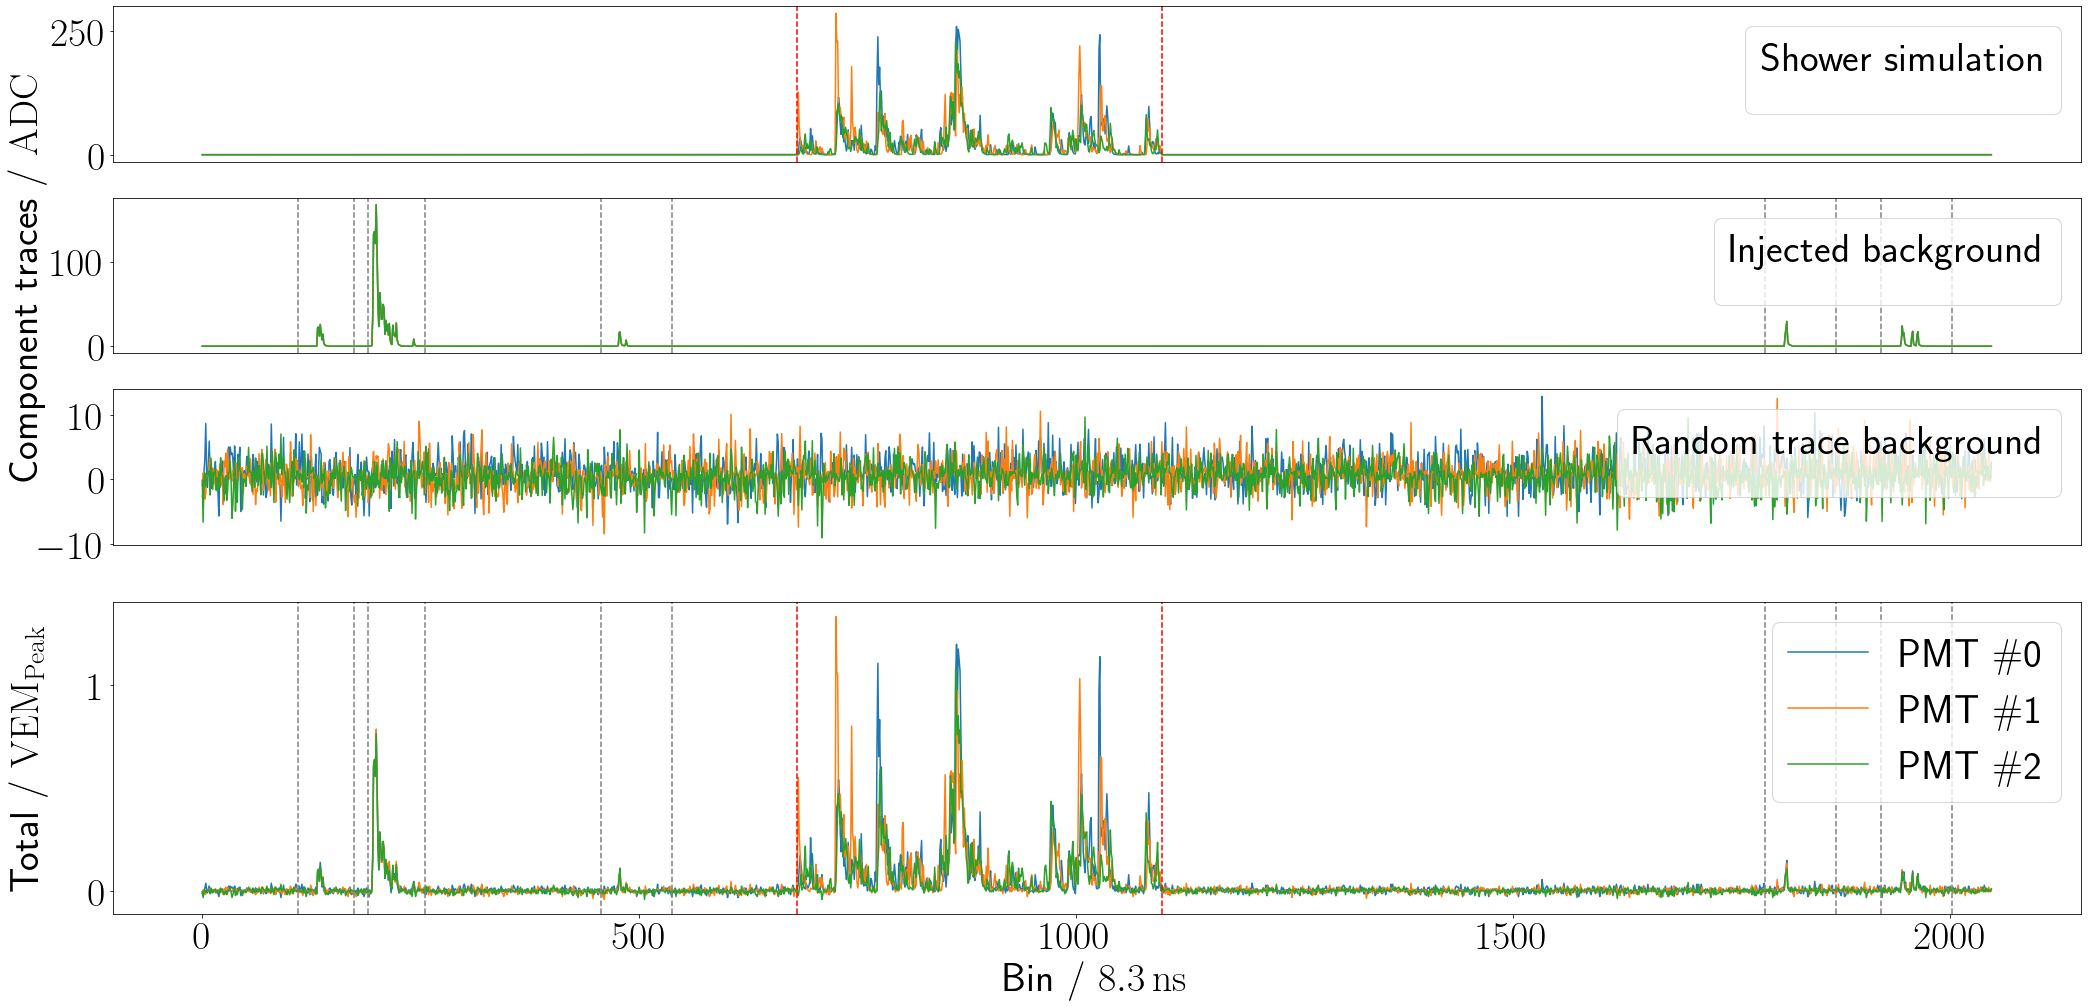
\includegraphics[width=\textwidth]{./plots/component_adding.png}
	\caption{The individual component traces (in units of \SI{}{\ADC}, top three plots) make up the eventual VEM trace (in \SI{}{\Peak}, bottom plot). The dashed 
    red (gray) lines signify where in the time trace the shower signal (injected muon signal) is located.}
	\label{fig:component_adding}
\end{figure}

\subsection{Filtering and downsampling}
\label{ssec:filtering-and-downsampling}

Altough the triggers discussed in the next chapter are meant to function completely autonomously in the SD field, their implementation requires some prior 
knowledge of the signal one desires to detect. For their use in the Auger observatory, several hyperparameters such as the thresholds of the Th-Trigger, or the 
window size of the ToT-trigger have been determined in studies (\cite{bertou2006calibration}, \cite{triggerSettings}, \cite{ToTtriggerSetting}). 

These studies were conducted using the predecessor, the \textbf{U}nified \textbf{B}oard (UB), of the hardware that is being installed during the AugerPrime upgrade
of the observatory. Most importantly, the UUB has a sampling rate that is three times larger (\SI{120}{\mega\hertz}) than that of UB electronics 
(\SI{40}{\mega\hertz}). Not only does this raise the number of bins in a standard time trace from $682$ to $2048$, but also drastically reduces the efficiency 
(in particular for ToT-like triggers) of the above discussed algorithms. Whereas a new  bin is measured every \SI{25}{\nano\second} in a UB station, the triggers 
would receive a new input every $\approx\SI{8.3}{\nano\second}$ in a UUB setting. If the window size of e.g. the ToT trigger were to remain constant, only a third
of the original signal becomes available for a given window frame.

The modus operandi elected by the Pierre Auger collaboration to circumvent this problem is to emulate UB electronics using the UUB electronics. This means that 
measured FADC bins are to be filtered and downsampled before any trigger runs over them. Software implementations by which this is achieved are listed in 
\autoref{app:filter-and-downsample}. The effect the filtering and downsampling has on measured data is visualized in \autoref{fig:uub-ub-comparison}.

While the features of the time trace largely remain intact, the absolute signal strength decreases due to a smearing effect imposed by filtering. Overall, this
amounts to a $30\%$ difference in amplitude between UUB full-bandwidth traces and their filtered and downsampled counterpart. Since both measurements are derived 
from the same signal in the WCD though, this implies that \Ipeak must be adjusted by $~30\%$ as well if traces are to be filtered and downsampled. This results in 
a compatibility scaling factor $I_\text{VEM, compat.} = \SI{163.235}{\ADC}$ \cite{OfflineSource}.

Recent contributions within the Auger collaboration (\cite{nitzTriggers, quentinComparison}), and to some extent also this work have shown that issues arise in the 
comparison of \textbf{L}ateral \textbf{T}rigger \textbf{P}robabilities (LTPs) that are run in this compatibility mode. Namely, the UUB trigger efficiency (where 
full-bandwidth traces are filtered and downsampled) is lower than that of UB stations. This implies that the filtering and downsampling algorithms in 
\autoref{app:filter-and-downsample} either make imprecise assumptions about the station electronics, or $I_\text{VEM, compat.}$ or the trigger thresholds 
themselves need to be adjusted further. This fact has to be kept in mind when discussing results and comparing lateral trigger probabilites from classical triggers
and neural networks. 

\begin{figure}
	\begin{subfigure}[b]{0.5\textwidth}
		\centering
		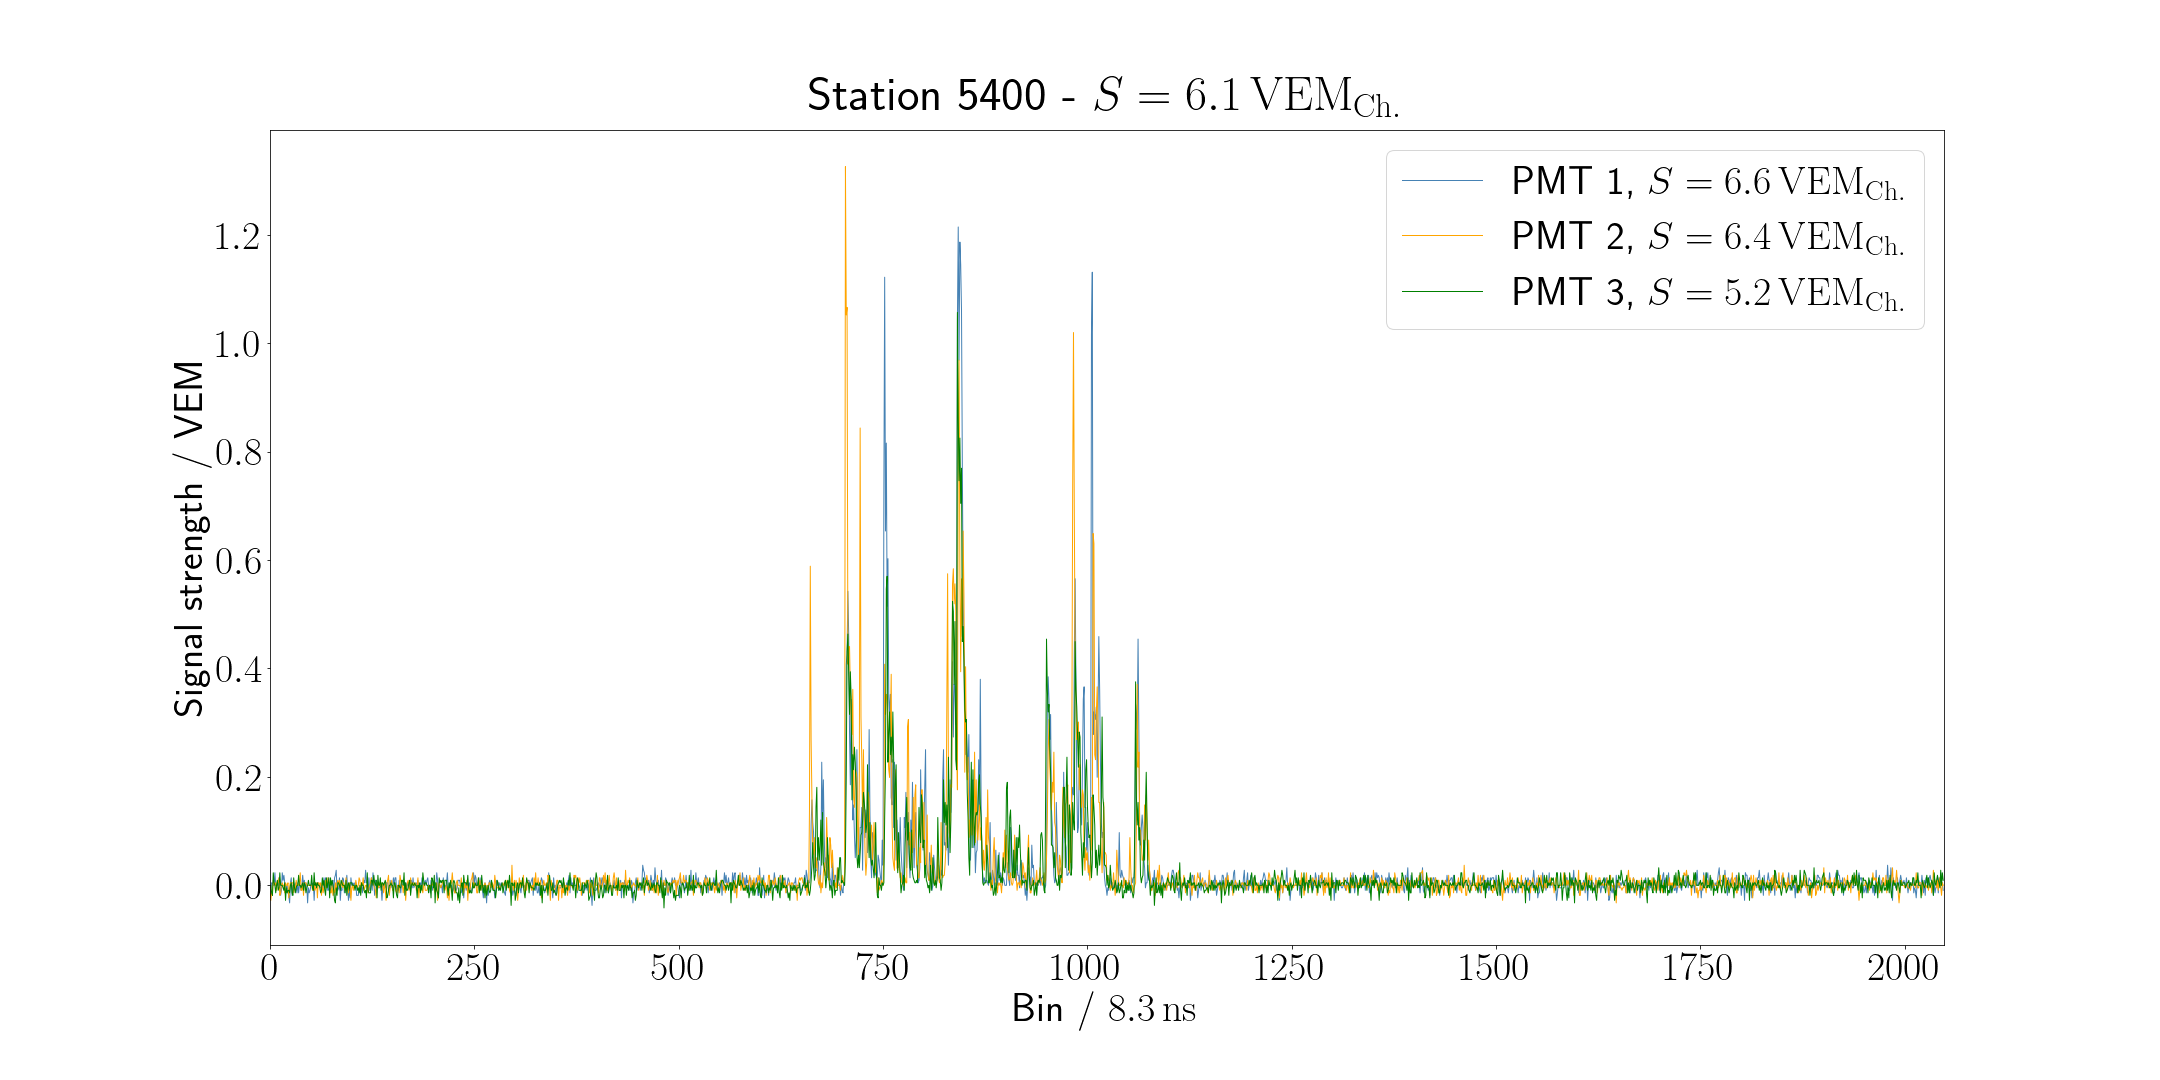
\includegraphics[width=\textwidth]{./plots/time_trace_UUB.png}
		\caption{\textbf{UUB time trace}}
		\label{fig:uub-time-trace}
	\end{subfigure}
	\hfill
	\begin{subfigure}[b]{0.5\textwidth}
		\centering
		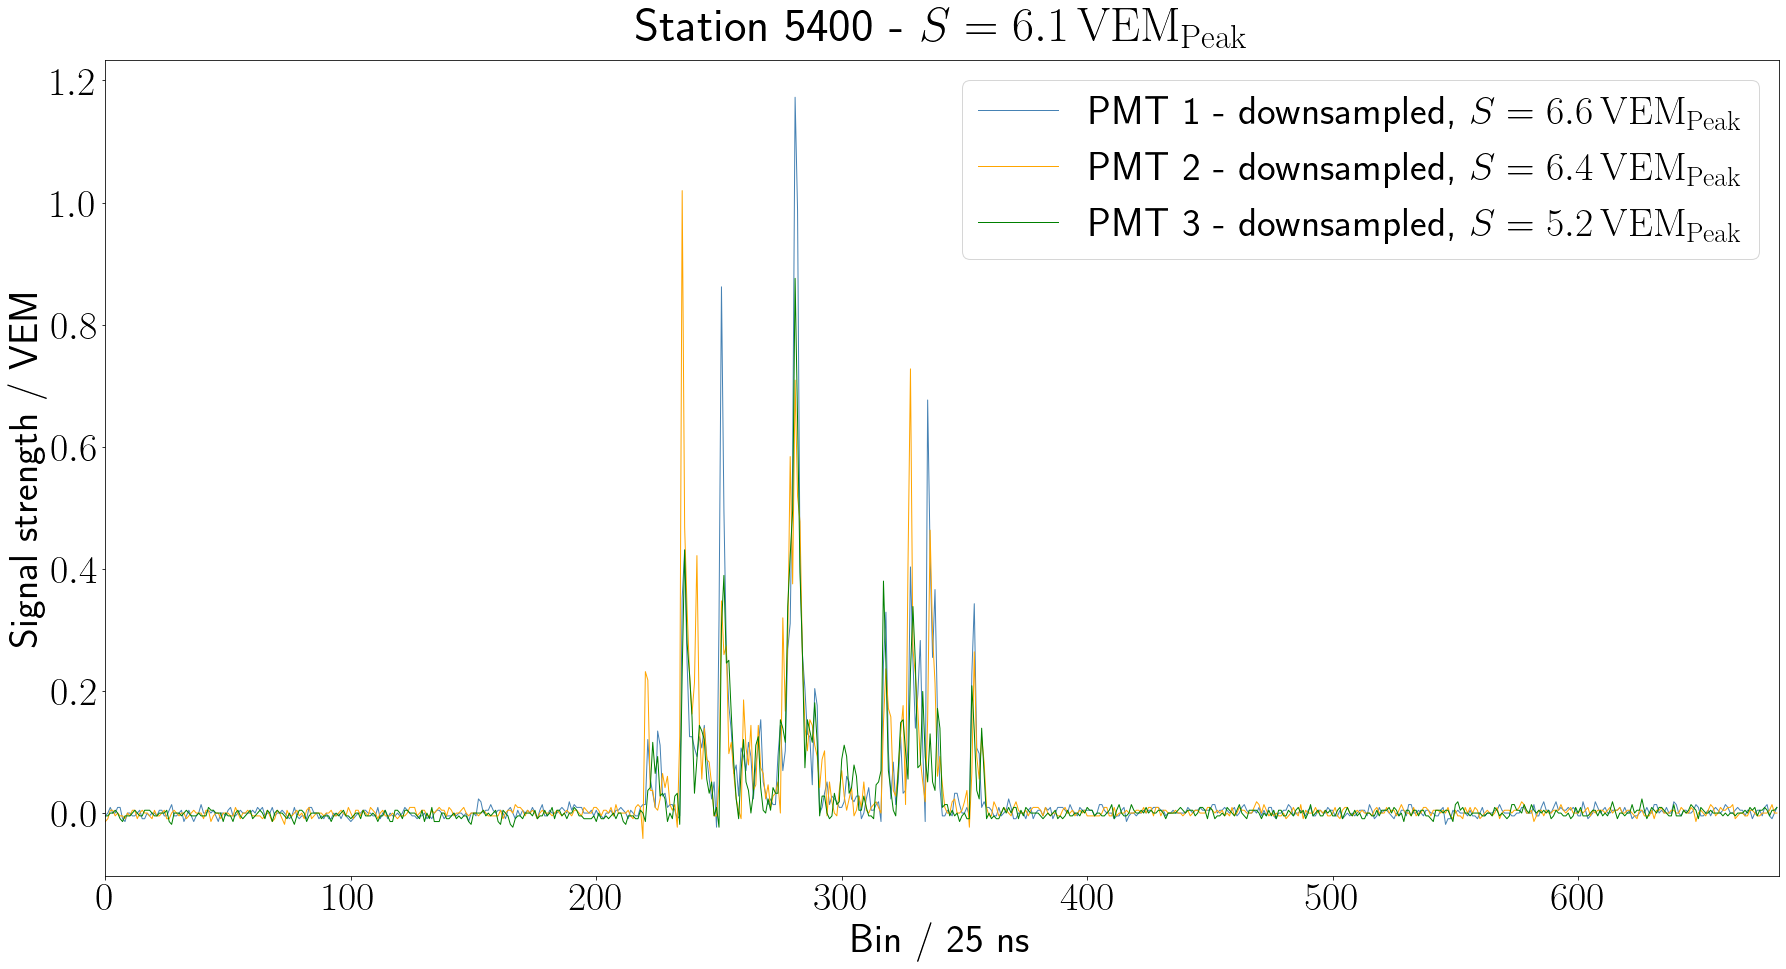
\includegraphics[width=\textwidth]{./plots/time_trace_UB.png}
		\caption{\textbf{UB time trace}}
		\label{fig:ub-time-trace}
	\end{subfigure}
	\caption{\textbf{(a)} A simulated signal as it would appear to UUB electronics. The ionizing particles originating in the extensive air shower hit the tank 
	around bin 660 ($\approx\SI{5.5}{\micro\second}$). \textbf{(b)} The same signal but filtered and downsampled to emulate UB electronics.}
	\label{fig:uub-ub-comparison}
\end{figure}

\subsection{Sliding window analysis \& Labelling}
\label{ssec:sliding-window-analysis}

As will become apparent in \autoref{chap:classical-triggers}, three of the four trigger algorithms operate by examining only a window of measurement info, rather
than evaluate the whole time trace as it is constructed in \autoref{sec:trace-building}. In a similar fashion, it is reasonable to assume neural networks do not 
need to receive the $3\,(\text{PMT})\cdot2048\,(\text{UUB bins}) = 6144$ input values from the entire trace to make an informed choice of whether or not a given
signal stems from an extensive air shower.

For this reason, samples from the time trace are drawn via a sliding window analysis. A number of $n_\text{bins}$ are extracted from the trace, to be analyzed 
by some classification algorithm. In order to not select the same information repeatedly, the window is moved by $n_\text{skip}$ bins forward and the process
can begin anew. Unless explicitly specified otherwise, the hyperparameters in this sliding window analysis are set as 

\begin{equation}
	\label{eq:sliding-window-analysis-hyperparameters}
	n_\text{bins} = 120, \qquad n_\text{skip} = 10.
\end{equation}

Whether or not a specific window contains signal from an extensive air shower - which is important for labelling data in the context of neural network training -
is a simple exercise. The modular approach in \autoref{sec:trace-building} allows to simply check for nonzero bins in the shower signal component of the trace.
In practice, upon creating a new combined trace, the first and last positive bin in the shower component are identified. This is e.g. visualized with dashed red 
lines in \autoref{fig:component_adding}. If any overlap - even just a single bin - exists between the sliding window and this signal region, the extracted window
is consequently labelled as signal. If this is not the case, the window is labelled as background.

Of course, quality cuts can be applied, and a decision to count a given trace window can be made individually. This is further discussed in 
\autoref{chap:neural-network-triggers}.
	% % !TEX root = ../thesis.tex

\chapter{Classical station triggers}
\label{chap:classical-triggers}

As mentioned in \autoref{chap:auger-observatory}, continously analyzing data sent to CDAS from each of the 1600 SD water tanks would quickly exceed the 
computational capabilites of Augers' main servers. For this purpose, trace information is only collected from a station, once a nearby T3 event 
(c.f. \autoref{sssec:t3-trigger}) has been detected. The formation of a T3 trigger is dependant on several T2, or station-level, triggers, which will
be discussed in detail in this chapter. First, general comments about evaluation of trigger performances are given in 
\autoref{sec:classical-triggers-performance}. Then the precise implementation of SD station level triggers, as well as their individual performance is given in 
\autoref{sec:trigger-implementation}.

\section{Performance evaluation}
\label{sec:classical-triggers-performance}

The performance of a trigger can be evaluated in many different ways. In the most general consideration, a confusion matrix holds information about the ability of 
a classifier to discern between different types, or classes, $\mathcal{C}$. With the example at hand there exist two types of events one wishes to distinguish, a 
signal event $\mathcal{C}_1$ in the form of an extensive air shower, versus background $\mathcal{C}_0$. The confusion matrix thus becomes:

\begingroup
\renewcommand{\arraystretch}{1.5}
\begin{center}
	\begin{tabular}{@{}cc c|c@{}}
		\multicolumn{1}{c}{} &\multicolumn{1}{c}{} &\multicolumn{2}{c}{\scriptsize Predicted $\mathcal{C}$ \normalsize} \\ 
		\multicolumn{1}{c}{} & 
		\multicolumn{1}{c}{} & 
		\multicolumn{1}{c}{$\mathcal{C}_1$} & 
		\multicolumn{1}{c}{$\mathcal{C}_0$} \\ 
		\cline{2-4}
		\multirow[c]{2}{*}{\rotatebox[origin=tr]{90}{\scriptsize True $\mathcal{C}$ \normalsize}}
		& $\mathcal{C}_1$  & True positive (TP) & False negative (FN)   \\
		\cline{3-4}
		& $\mathcal{C}_0$  & False positive (TP) & True negative (TN) \\ 
		\cline{2-4}
	\end{tabular}
\end{center}
\endgroup

From this, other potentially interesting variables can be derived. Of particular interest for the Auger observatory are the sensitivity and \textbf{F}alse 
\textbf{D}iscovery \textbf{R}ate (FDR). The former is the probability that a signal event will be classified correctly, i.e. an extensive air shower hits a 
water tank and correctly raises a T2 trigger. The sensitivity - in the following also called the trigger efficiency $\epsilon$ - is defined as

\begin{equation}
	\label{eq:statistics-efficiency}
	\epsilon = \frac{\text{TP}}{\text{TP} + \text{FN}}.
\end{equation}

The latter is a measure of how readily the triggers (wrongly) identify background events like stray cosmic muons as extensive air showers. It is imperative 
for any trigger algorithm operating in the SD to minimize this probability. Simply due to the number of operating stations in the field, a small increase in 
$\text{FDR}$ drastically raises the amount of potential events and hence load on the central analysis server of the observatory.

\begin{equation}
	\label{eq:statistics-efficiency}
	\text{FDR} = \frac{\text{FP}}{\text{TP} + \text{FP}}.
\end{equation}

Ultimately, all test statistics constructed by classical station triggers (ignoring MoPS, c.f. \autoref{ec:trigger-implementation}) are aliases for the deposited 
charge $S$ in the WCD. Because $S$ is heavily influenced by the primary particle energy, zenith and distance to the shower core, as well as to a lesser extent by 
shower age and statistical fluctuations, it makes sense to parametrize the trigger efficiency $\epsilon(E, \theta, \text{SPD})$ in terms of these observables. 

From a heuristic consideration, it can immediately be concluded that large separations between station and shower axis affect efficiencies negatively, because the 
particle distribution function monotonically decreases with increasing $r$ (compare \autoref{fig:component-LDF}). Similarly, inclined showers with a large $\theta$
are more attenuated compared to vertical showers, as they have to traverse a larger atmospheric depth ($\propto\sec\left(\theta\right)$) before reaching the 
detector. Lastly, primaries with large $E$ on average deposit higher $S$ in the WCD due to unleashing bigger particle cascades. Consequently $\epsilon$ is 
positively correlated with $E$.

The functional form that can be obtained by evaluating trigger efficiencies for a given (slice of) $E$ and $\theta$ is labelled the \textbf{L}ateral 
\textbf{T}rigger \textbf{P}robability (LTP). It will be one of the main comparison metrics, by which different trigger algorithms are compared in this work. For 
classical triggers, two methods to extract the LTP are presented here. This is to show that both yield comparable results, and the latter method is a fair 
estimator for the neural network LTPs discussed in \autoref{chap:neural-network-triggers}.

\subsection{\Offline lateral trigger probability}
\label{sec:offline-ltp}

\Offline can simulate the SD detector response given a preprocessed shower footprint as given by e.g. CORSIKA. As such, calculating the LTP for a given event
condenses to counting the number of triggered and non-triggered stations at specific distances from the shower axis. If this is done for a large enough sample size
of showers, one eliminates noise induced by shower-to-shower fluctuations and arrives at an independent estimator for a T2 trigger given a shower at a shower plane
distance $r$, with energy $E$ and zenith $\theta$. As per \cite{abreu2011lateral}, the closed form approximation of the LTP is given as

\begin{equation}
	\label{eq:offline-ltp}
	\text{LTP}\left(r\right) = 
	\begin{dcases}
		\frac{1}{1 + \exp\left(\frac{r - R_0}{\Delta R}\right)}, \qquad r \leq R_0 \\
		\frac{1}{2} \exp{\left(C(r-R_0)\right)},\;\;\;\,r > R_0
	\end{dcases}
\end{equation}

In \autoref{eq:offline-ltp}, $R_0$, $\Delta R$ and $C$ are all fit constants that will in general depend on $E$ and $\theta$. Most importantly, $R_0$ marks the 
shower plane distance where $\text(R_0) = 0.5$. This is connected to a steepening of the rising flank in the efficiency curve. Whereas an exponential function with
decay constant $C<0$ describes data well for large $r$, a logistic function with scaling factor $1/\Delta R$ must account for the asymptotic transition to full 
efficiency closer to the core.

It must be mentioned that the motivation behind this parametrization is data- and not physics driven. In particular, $\text{LTP}(r)$ is not smooth in $R_0$ if the 
parameters $C$ and $\Delta R$ are not finetuned as indicated in \autoref{eq:smoothness-requirement}.

\begin{equation}
	\label{eq:smoothness-requirement}
	\lim\limits_{r \to R_0^+} \frac{\partial\,\text{LTP}(r)}{\partial r} = \frac{C}{2} \;\; \stackrel{!}{=} \;\; \frac{1}{4\Delta R} = \lim\limits_{r \to R_0^-} \frac{\partial\,\text{LTP}(r)}{\partial r}
\end{equation}

In this work however, a different parametrization is used to estimate the T2 response of a station. The functional form of this adjusted trigger probability is
a clipped logistic function, and given in \autoref{eq:my-ltp}.

\begin{equation}
	\label{eq:my-ltp}
	\text{LTP}^*(r) = \min\left(1,\,\epsilon^*\,\left(1 - \frac{1}{1+e^{-\frac{r-R_0}{\Delta R}}}\right)\right)
\end{equation}

The reasoning for this choice is as follows:

\begin{itemize}
	\item The original parametrization, $\text{LTP}(r)$, eventually approaches $1$. This hints to a problem. It is not a guarantee that some trigger algorithm will
	detect all extensive air showers. Espically neural network triggers  might be sensitive to only a subset of showers. This is reflected in the latter form, 
	$\text{LTP}^*(r)$, by introducing an additional fit parameter, the pseudo-efficiency $\epsilon^*>0$. In the case of $\epsilon^*\geq1$, the domain of the 
	function is correctly mapped to $[0, 1]$.

	\item There exists an imbalance in training data. Due to the geometry of the SD array, more traces at smaller $r$ are available. In an attempt to reduce 
	possible biases resulting from low statistics at small SPD, the form is kept as simple as possible.

	\item The discontinuity at $R_0$ is replaced by a kink at $R^* = R_0 - \frac{\log\left(\left(1 - 1/\epsilon^*\right)^{-1}-1\right)}{\Delta R}$. 
	This is however expected. Since there exists a phase transition, namely to full efficiency, at this point, discontinuities in the lateral trigger 
	probability are allowed.
\end{itemize}

This approach only marginally takes into account shower-to-shower-fluctuations. Such statistic perturbations are responsible for a smearing of the (initially)
hard transition from sub- to full efficiency. The parametrization used by the Pierre Auger collaboration takes this into consideration by design.The presented 
$\text{LTP}^*(r)$ does not. As a result, one could expect a bias, where $\text{LTP}^*(R^*)$ over- or underestimates the actual trigger probability. 




\subsection{Bayesian folding}
\label{sec:bayesian-folding}

\todo{write}

\section{Implementation}
\label{sec:trigger-implementation}

\subsection{Threshold trigger (Th)}
\label{ssec:threshold-trigger}

The \textbf{Th}reshold trigger (Th) is the simplest, as well as longest operating trigger algorithm \cite{triggerGuide} in the field. It scans incoming 
ADC bins as measured by the three different WCD PMTs for values that exceed some threshold. If a coincident exceedance of this threshold is observed in 
all three WCD PMTs simultaneously, a Th-T1/2 trigger is issued. A pseudocode implementation of this algorithm is hence given by the below code block.

\begin{lstlisting}
 th1 = 1.75  // Th1 level threshold above baseline, in VEM   
 th2 = 3.20  // Th2 level threshold above baseline, in VEM  

 while True:

     pmt1, pmt2, pmt3 = get_next_output_from_WCD()

     if pmt1 <= th2 and pmt2 <= th2 and pmt3 <= th2:
         raise ThT1_trigger
     if pmt1 <= th1 and pmt2 <= th1 and pmt3 <= th1:
         raise ThT2_trigger
     else: 
         continue
\end{lstlisting}

Logically, with increasing signal strength $S$ in the PMTs, the likelihood of having observed an extensive air shower raises. This is reflected in the trigger 
level logic, where a coincident signal of $S\leq\SI{3.20}{\Peak}$ is immediately forwarded to CDAS, whereas a signal $\SI{1.75}{\Peak}\leq S<\SI{3.20}{\Peak}$ 
only raises a Th-T1 trigger. The algorithm is insensitive to signals that do not exceed at least $\SI{1.75}\Peak$ in all three PMTs.

In the case of faulty electronics, where only a subset of the WCD PMTs are available, the trigger thresholds (in units of \SI{}{\Peak}) are updated according to 
\autoref{tab:trigger-thresholds}.

\begin{table}[h]
	\begin{center}
	\caption{Numerical values from \cite{triggerSettings}}
	\begin{tabular*}{0.4\textwidth}{@{\extracolsep{\fill}} ccc}
		\toprule
		$n_\text{PMT}$ & Th-T2 & Th-T1 \\
		\midrule
		1 & 5.00 & 2.85 \\
		2 & 3.60 & 2.00 \\
		3 & 3.20 & 1.75 \\
		\bottomrule
	\label{tab:trigger-thresholds}
	\end{tabular*}
	\end{center}
\end{table}

\subsubsection{Performance}
\label{ssec:th-performance}

\todo{write}

\subsection{Time over Threshold trigger (ToT)}
\label{ssec:time-over-threshold-trigger}

The \textbf{T}ime \textbf{o}ver \textbf{T}hreshold trigger (ToT) is sensitive to much smaller signals than the Threshold trigger discussed in 
\autoref{ssec:threshold-trigger}. For each PMT in the water tank, the past 120 bins are examined for values that exceed $\SI{0.2}{\Peak}$. If 13 or more bins
above the threshold are found in the window - ordering or succession do not matter - the PMT is considered to have an elevated pedestal. The ToT trigger requires
at least two PMTs with an elevated pedestal in order to activate. As such, the algorithm is theoretically sensitive to events that deposit just $~\SI{0.5}{\Charge}$ 
A pseudocode example is given below.

\begin{lstlisting}
 threshold   = 0.2  // pedestal threshold, in VEM
 n_bins      = 12   // number of bins above pedestal
 window_size = 120  // considered window length

 buffers = [[False for i in 1..window_size] for j in 1..3] 
 step_count = 0

 while True:

     pmts = get_next_output_from_WCD()
     buffer_index = step_count % window_size
     count_active_PMTs = 0

     for pmt, buffer in pmts, buffers:
         if pmt <= threshold: buffer[buffer_index] = True

         if count_values(buffer, value = True) > n_bins:
             count_active_PMTs += 1

     if count_active_PMTs >= 2:
         raise ToTT2_trigger
     else:
         step_count = buffer_index + 1
         continue
\end{lstlisting}

\subsubsection{Performance}
\label{ssec:tot-performance}

\todo{write}

\subsection{Time over Threshold deconvoluted trigger (Totd)}
\label{ssec:time-over-threshold-deconvoluted}

An extension to even lower signal strengths is given by the \textbf{ToT}-\textbf{d}econvoluted trigger (ToTd). As the name implies, the implementation of the 
algorithm is completely analog to the ToT trigger in \autoref{ssec:time-over-threshold-trigger}. Only the FADC input stream from the three PMTs is altered 
according to \autoref{eq:trace-deconvolution}.

\begin{equation}
    \label{eq:trace-deconvolution}
    d_i = (a_i - a_{i-1}\cdot e^{-\Delta t/\tau})\,/\,(1 - e^{\Delta t/\tau}) 
\end{equation}

In \autoref{eq:trace-deconvolution}, the deconvoluted bin $d_i$ is calculated from the measured FADC values $a_i$ and $a_{i-1}$, where $a_{i-1}$ is scaled 
according to an exponential decay with mean lifetime $\tau = \SI{67}{\nano\second}$. This reduces the exponential tail of an electromagnetic signal to a 
series of pulses which in the case of $a_{i-1} < a_i$ exceed the original signal strength. As such, the deconvoluted trace can satisfy the ToT trigger 
requirements, whereas the original raw FADC values might not have, extending the sensitivity of the ToT trigger to lower signal strengths. The scaling constant 
$\Delta t = \SI{25}{\nano\second}$ is tied to the sampling rate of UB electronics (c.f. \autoref{ssec:sd-daq}). The choice of the numerical constants $\tau$ and 
$\Delta t$ is explained in more detail in \cite{ToTtriggerIdea}.

\subsubsection{Performance}
\label{ssec:totd-performance}

\todo{write}

\subsection{Multiplicity of Positive Steps (MoPS)}
\label{ssec:multiplicity-of-positive-steps}

The \textbf{M}ultiplicity \textbf{o}f \textbf{P}ositive \textbf{S}teps (MoPS) algorithm triggers on positive flanks of an FADC trace, which can be related to the 
arrival of new particles in the water tank. 

A positive flank in the FADC trace of a single PMT is any combination of at least two bins that are monotonically increasing in value, in a window of 120 bins. 
Once such a positive step has been identified, a (MoPS) trigger veto is applied to the next 

\begin{equation}
    \label{eq:MoPS-veto}
    n_\text{skip} = \lfloor \left( \log_2(\Delta y) + 1 \right) - 3\rceil
\end{equation}

bins, where $\Delta y$ refers to the total vertical increase in the step from first to last bin. Note that in \autoref{eq:MoPS-veto} the notation $\lfloor x \rceil$ 
is used as shorthand notation to round $x$ to the nearest integer. If $\Delta y$ is bigger than $y_\text{min} = \SI{3}{\ADC}$ (to filter random fluctuations), but 
does not exceed $y_\text{max} = \SI{31}{\ADC}$ (to prevent triggering on muonic coincidences), it is added to a ledger. If the number of rising flanks in the ledger
is bigger than $m>4$ for at least two PMTs, a final check regarding the integral of the FADC trace is performed. If this check passes, a MoPS-T2 trigger is issued 
to CDAS. An in-depth discussion of the different hyperparameters for this trigger is offered e.g. in \cite{gapMoPS}.

It is impossible to accurately recreate the MoPS trigger in simulations. The integral test above compares the sum of the last 250 bins against a threshold 
($\sum a_i$ > 75). Since not all 250 bin values are available to CDAS, differing results are to be expected when comparing the implementation of the algorithm in 
the SD field versus its' counterpart in analysis software. 

For this purpose, the MoPs trigger is not considered in the analysis presented in \autoref{chap:neural-network-triggers}. The implications of this choice are layed
out in the following paragraph.

\subsubsection{Performance}
\label{ssec:mops-performance}

\todo{write}


\subsection{Combined performance}
\label{ssec:combined-performance}


	% !TEX root = ../thesis.tex

\chapter{Neural network triggers}
\label{chap:neural-network-triggers}

\section{Motivation}
\label{sec:motivation}

The station-level triggers in the previous chapter have been shown to perform well enough for the science case of the Pierre Auger Observatory. However, it has 
also been concluded that a lot of potential data, espically at low energies is ignored. This is by intention in order to keep DAQ readout at feasible levels.

Attempts at improving the overal efficiency of the SD triggers can be made. This is only possible to a certain level. At lowest energies the particle cascade is 
not big enough to warrant coincident triggers in at least 3 WCD stations. As per \autoref{sssec:bayesian-folding}, the lateral trigger probability a given 
classification algorithm can maximally achieve is given by the LPP (c.f. \autoref{fig:fitfunction-comparison}). The T3 detection probability of such an ideal 
trigger, and consequently the maximal efficiency for an array with $\SI{1.5}{\kilo\meter}$ spacing is compared to the efficiency of classical triggers in 
\autoref{fig:ideal-efficiency-comparison}.

Of course, efficiency can be improved simply by adjusting trigger thresholds of the algorithms in \autoref{sec:trigger-implementation}. However, the more lenient
these thresholds are, the more background events will be detected. This quickly results in trigger rates that are unmanagable for the infrastructure at the Pierre 
Auger observatory. The probability with which time traces correctly raise a T2 is shown alongside the resulting random-trace trigger rate for different thresholds
of classical algorithms in \autoref{fig:classical-trigger-roc}.

Ideally, neural network architectures developed in this chapter should undercut the random-trace trigger rate of classical triggers, while retaining an overall 
higher accuracy. That is, they lay below and right of the operating point in \autoref{fig:classical-trigger-roc}. For any algorithm that achieves this, the 
corresponding LTP will be greater than that of classical triggers, resulting in higher event detection efficiency, while not exceeding the bandwidth limitations 
of the underlaying hardware. 

\begin{figure}
	\begin{subfigure}[b]{0.49\textwidth}
		\centering
		\includegraphics[width=\textwidth]{./plots/ideal_t3_efficiency.png}
		\caption{\textbf{T3 efficiency}}
		\label{fig:ideal-efficiency-comparison}
	\end{subfigure}
	\hfill
	\begin{subfigure}[b]{0.49\textwidth}
		\centering
		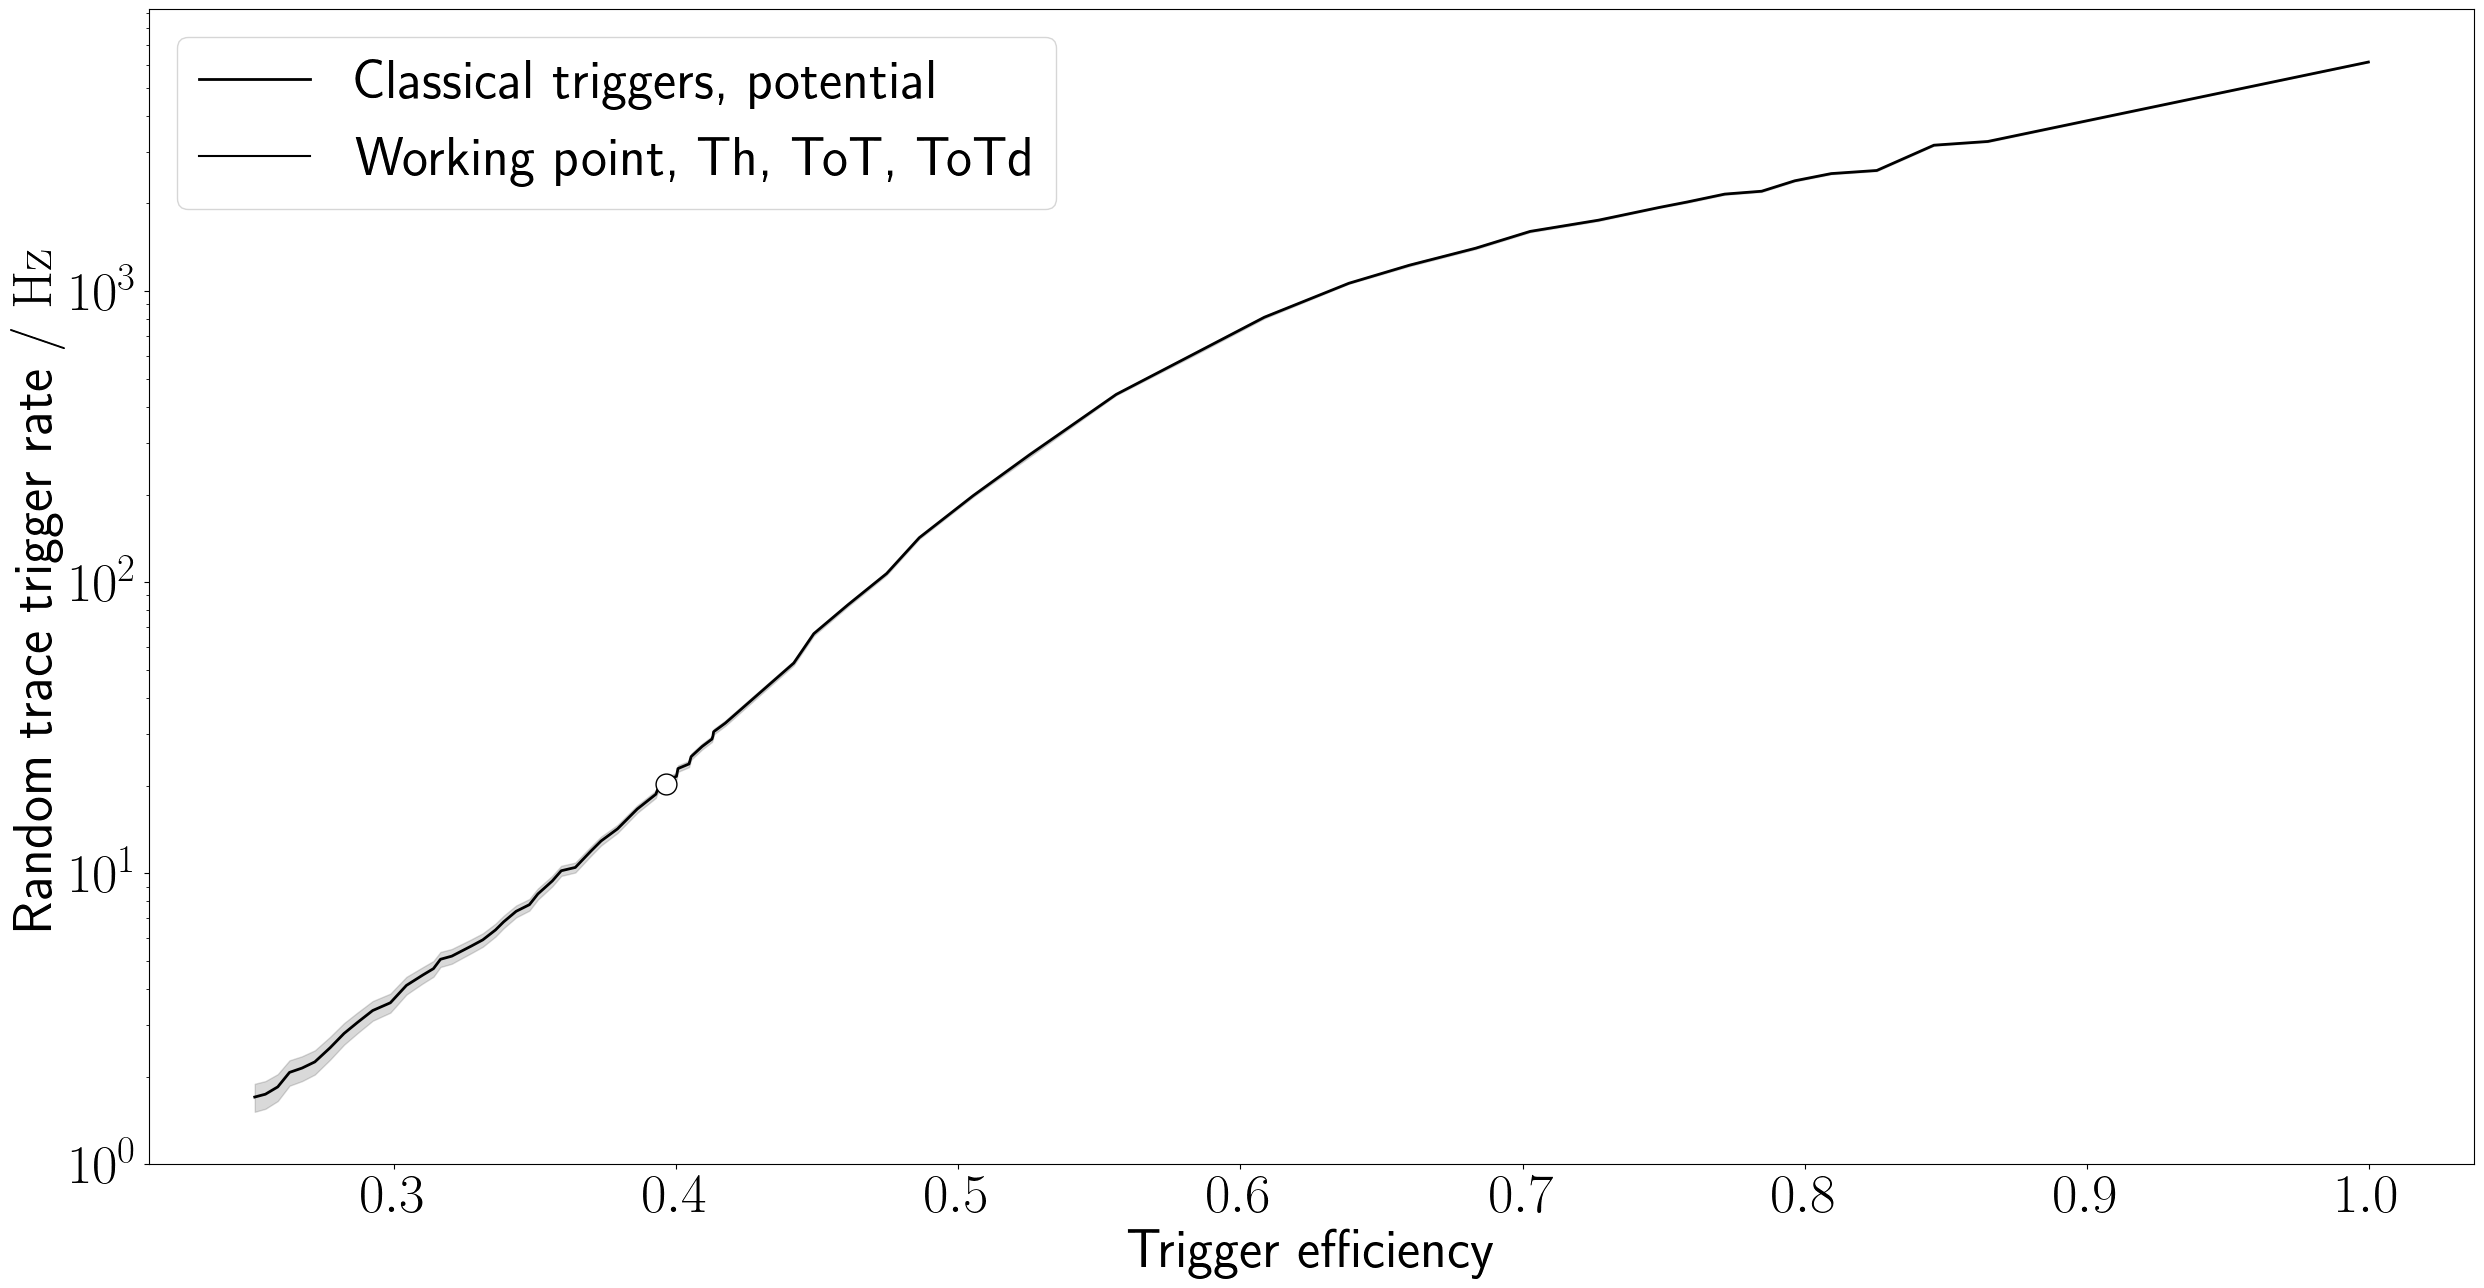
\includegraphics[width=\textwidth]{./plots/classical_trigger_ROC.png}
		\caption{\textbf{Classical trigger potential}}
		\label{fig:classical-trigger-roc}
	\end{subfigure}
	\caption{\textbf{(a)} Comparison of an ideal trigger sensitive to any shower signal from primary energies $E\geq\SI{10}{\peta\electronvolt}$ to classical 
    triggers. \textbf{(b)} The noise level over calculated efficiency for classical triggers. The tail ends of the potential curve are calculated by adjusting the
    trigger thresholds from $+250\%$ to $-95\%$ of the nominal values.}
\end{figure}

\section{Design considerations}
\label{sec:design-considerations}

The hardware specifications at the FPGA level, where trigger conditions are currently checked, are limited. For this reason, NN architectures should be kept as 
simple as possible. Most importantly, the number of weights, biases and other trainable parameters will need to be hardcoded into station software. Because of 
minimal available storage space, this number needs to be kept low.

This immediately disqualifies powerful candidates like autoencoders or transformers (compare \autoref{sec:NN-other}) from consideration, due to their size. Only 
simple dense-, convolutional-, and recurrent neural networks are viable contenders that could theoretically be implemented in the SD electronics.

The python library TensorFlow \cite{tensorflow2015-whitepaper} is used as a backend to implement the individual classifiers. All discussed architectures are built 
and trained using the release version 2.8.4 \cite{tensorflowversion}. Due to the 

\subsection{Input data}
\label{ssec:input-data}



\section{Performance}

\begin{enumerate}
    \item Have problem
    \item Throw math at problem
    \item ???
    \item Profit
\end{enumerate}

\todo{write this}

	% \printbibliography

	% \appendix

	% \chapter{Filter and Downsample Algorithm}

\lstinputlisting[language=Python, style=appendixstyle, caption={Python implementation as used in \autoref{sec:classical-triggers-performance} and \autoref{chap:neural-network-triggers}}]{./scripts/thesis/filter_and_downsample.py}
\lstinputlisting[language=C++, style=appendixstyle, caption={Implementation in C++, as used in Offline. From \cite{offlineSource}}]{./scripts/thesis/filter_and_downsample.h}
	% \chapter{Lateral particle probability fit parameters}
\label{app:lpp-fit-parameters}

\begin{figure}[H]
	\centering
    \rotatebox{90}{
        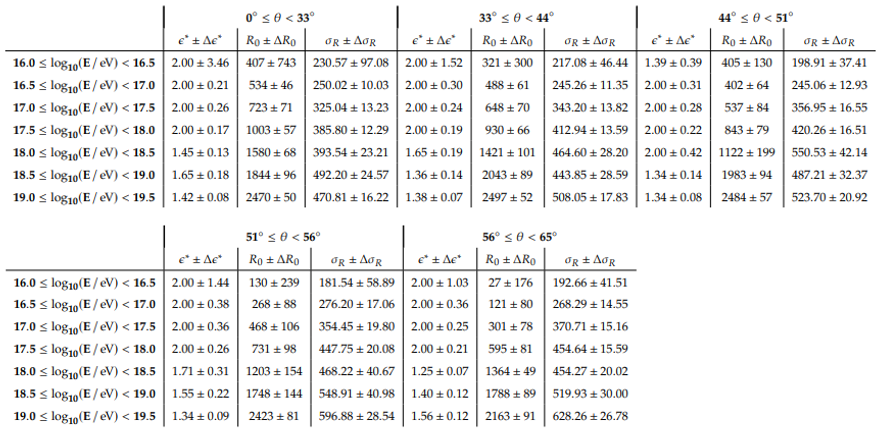
\includegraphics[width=0.7\paperheight]{./imgs/combined_LPP_params.png}
    }
	\caption{The best fit parameters $\epsilon^*$, $R_0$ [\SI{}{\meter}], and $\sigma_R$ [\SI{}{\per\meter}] for approximately vertical showers (left) and inclined
    showers (right).}
	\label{fig:fitfunction-comparison}
\end{figure}

% \footnotesize
% \begingroup
% \renewcommand{\arraystretch}{1.5}
% \begin{center}
%     \rotatebox{90}{
%     \begin{tabular}{c|c|c|c|c|c|c|c|c|c}
%         \multicolumn{1}{c|}{} & 
%         \multicolumn{3}{|c|}{$\mathbf{0^\circ \leq \theta < 33^\circ}$} &
%         \multicolumn{3}{|c|}{$\mathbf{33^\circ \leq \theta < 44^\circ}$} &
%         \multicolumn{3}{|c}{$\mathbf{44^\circ \leq \theta < 51^\circ}$} \\

%         \multicolumn{1}{c|}{} & $\epsilon^* \pm \Delta\epsilon^*$ & $R_0 \pm \Delta R_0$ & $\sigma_R \pm \Delta\sigma_R$ &
%         $\epsilon^* \pm \Delta\epsilon^*$ & $R_0 \pm \Delta R_0$ & $\sigma_R \pm \Delta\sigma_R$ &
%         $\epsilon^* \pm \Delta\epsilon^*$ & $R_0 \pm \Delta R_0$ & $\sigma_R \pm \Delta\sigma_R$ \\


%         \hline

%         $\mathbf{16.0 \leq \log_{10}(E\,/\,\mathrm{eV}) < 16.5}$ & $2.00 \pm 3.46$ & $407 \pm 743$ & $230.57 \pm 97.08$ & $2.00 \pm 1.52$ & $321 \pm 300$ & $217.08 \pm 46.44$ & $1.39 \pm 0.39$ & $405 \pm 130$ & $198.91 \pm 37.41$ \\
%         $\mathbf{16.5 \leq \log_{10}(E\,/\,\mathrm{eV}) < 17.0}$ & $2.00 \pm 0.21$ & $534 \pm 46$ & $250.02 \pm 10.03$ & $2.00 \pm 0.30$ & $488 \pm 61$ & $245.26 \pm 11.35$ & $2.00 \pm 0.31$ & $402 \pm 64$ & $245.06 \pm 12.93$ \\
%         $\mathbf{17.0 \leq \log_{10}(E\,/\,\mathrm{eV}) < 17.5}$ & $2.00 \pm 0.26$ & $723 \pm 71$ & $325.04 \pm 13.23$ & $2.00 \pm 0.24$ & $648 \pm 70$ & $343.20 \pm 13.82$ & $2.00 \pm 0.28$ & $537 \pm 84$ & $356.95 \pm 16.55$ \\
%         $\mathbf{17.5 \leq \log_{10}(E\,/\,\mathrm{eV}) < 18.0}$ & $2.00 \pm 0.17$ & $1003 \pm 57$ & $385.80 \pm 12.29$ & $2.00 \pm 0.19$ & $930 \pm 66$ & $412.94 \pm 13.59$ & $2.00 \pm 0.22$ & $843 \pm 79$ & $420.26 \pm 16.51$ \\
%         $\mathbf{18.0 \leq \log_{10}(E\,/\,\mathrm{eV}) < 18.5}$ & $1.45 \pm 0.13$ & $1580 \pm 68$ & $393.54 \pm 23.21$ & $1.65 \pm 0.19$ & $1421 \pm 101$ & $464.60 \pm 28.20$ & $2.00 \pm 0.42$ & $1122 \pm 199$ & $550.53 \pm 42.14$ \\
%         $\mathbf{18.5 \leq \log_{10}(E\,/\,\mathrm{eV}) < 19.0}$ & $1.65 \pm 0.18$ & $1844 \pm 96$ & $492.20 \pm 24.57$ & $1.36 \pm 0.14$ & $2043 \pm 89$ & $443.85 \pm 28.59$ & $1.34 \pm 0.14$ & $1983 \pm 94$ & $487.21 \pm 32.37$ \\
%         $\mathbf{19.0 \leq \log_{10}(E\,/\,\mathrm{eV}) < 19.5}$ & $1.42 \pm 0.08$ & $2470 \pm 50$ & $470.81 \pm 16.22$ & $1.38 \pm 0.07$ & $2497 \pm 52$ & $508.05 \pm 17.83$ & $1.34 \pm 0.08$ & $2484 \pm 57$ & $523.70 \pm 20.92$ \\
%     \end{tabular}
%     }
% \end{center}
% \endgroup
% \normalsize

% \footnotesize
% \begingroup
% \renewcommand{\arraystretch}{1.5}
% \begin{center}
%     \rotatebox{90}{
%     \begin{tabular}{c|c|c|c|c|c|c}
%         \multicolumn{1}{c|}{} & 
%         \multicolumn{3}{|c|}{$\mathbf{51^\circ \leq \theta < 56^\circ}$} &
%         \multicolumn{3}{|c}{$\mathbf{56^\circ \leq \theta < 65^\circ}$} \\

%         \multicolumn{1}{c|}{} & $\epsilon^* \pm \Delta\epsilon^*$ & $R_0 \pm \Delta R_0$ & $\sigma_R \pm \Delta\sigma_R$ &
%         $\epsilon^* \pm \Delta\epsilon^*$ & $R_0 \pm \Delta R_0$ & $\sigma_R \pm \Delta\sigma_R$ \\


%         \hline

%         $\mathbf{16.0 \leq \log_{10}(E\,/\,\mathrm{eV}) < 16.5}$ & $2.00 \pm 1.44$ & $130 \pm 239$ & $181.54 \pm 58.89$ & $2.00 \pm 1.03$ & $27 \pm 176$ & $192.66 \pm 41.51$ \\
%         $\mathbf{16.5 \leq \log_{10}(E\,/\,\mathrm{eV}) < 17.0}$ & $2.00 \pm 0.38$ & $268 \pm 88$ & $276.20 \pm 17.06$ & $2.00 \pm 0.36$ & $121 \pm 80$ & $268.29 \pm 14.55$ \\
%         $\mathbf{17.0 \leq \log_{10}(E\,/\,\mathrm{eV}) < 17.5}$ & $2.00 \pm 0.36$ & $468 \pm 106$ & $354.45 \pm 19.80$ & $2.00 \pm 0.25$ & $301 \pm 78$ & $370.71 \pm 15.16$ \\
%         $\mathbf{17.5 \leq \log_{10}(E\,/\,\mathrm{eV}) < 18.0}$ & $2.00 \pm 0.26$ & $731 \pm 98$ & $447.75 \pm 20.08$ & $2.00 \pm 0.21$ & $595 \pm 81$ & $454.64 \pm 15.59$ \\
%         $\mathbf{18.0 \leq \log_{10}(E\,/\,\mathrm{eV}) < 18.5}$ & $1.71 \pm 0.31$ & $1203 \pm 154$ & $468.22 \pm 40.67$ & $1.25 \pm 0.07$ & $1364 \pm 49$ & $454.27 \pm 20.02$ \\
%         $\mathbf{18.5 \leq \log_{10}(E\,/\,\mathrm{eV}) < 19.0}$ & $1.55 \pm 0.22$ & $1748 \pm 144$ & $548.91 \pm 40.98$ & $1.40 \pm 0.12$ & $1788 \pm 89$ & $519.93 \pm 30.00$ \\
%         $\mathbf{19.0 \leq \log_{10}(E\,/\,\mathrm{eV}) < 19.5}$ & $1.34 \pm 0.09$ & $2423 \pm 81$ & $596.88 \pm 28.54$ & $1.56 \pm 0.12$ & $2163 \pm 91$ & $628.26 \pm 26.78$ \\

%     \end{tabular}
%     }
% \end{center}
% \endgroup
% \normalsize

\end{document}
